\documentclass[10pt,=table]{beamer}

\usetheme[subsectionpage=none]{metropolis}
%\useoutertheme{infolines}
%HEADEEER
\makeatletter


%SECTION PAGES (HEAD then COMPLETE title)
\defbeamertemplate*{section page}{mytheme}[1][]{
  \centering
  \begin{minipage}{22em}
    \raggedright
    \usebeamercolor[fg]{section title}
    \usebeamerfont{section title}
    \insertsectionhead\\[-1ex]
    \vspace{1cm}
    \usebeamerfont{subsection title}
    \insertsection\\[-1ex]
    \usebeamertemplate*{progress bar in section page}
    \par
    \ifx\insertsubsectionhead\@empty\else%
      \usebeamercolor[fg]{subsection title}%
      \usebeamerfont{subsection title}%
      \insertsubsectionhead
    \fi
    \vskip0.8cm
    \ifstrempty{#1}{}{%
		    \includegraphics[width=\textwidth]{#1}%		
	}
           

  \end{minipage}
  \par
  \vspace{\baselineskip}
}
%SUBSECTIONN PAGE (only subsection title)

\makeatother


\usepackage{appendixnumberbeamer}
\usepackage{booktabs}
\usepackage{multirow}
\usepackage{forest} 
\usepackage{adjustbox}
\usepackage{mathtools}
\usepackage{tikz}
\usepackage{xcolor}
\definecolor{greenEric}{HTML}{297373}
\newcommand*\circled[1]{\tikz[baseline=(char.base)]{
            \node[shape=circle,draw,inner sep=1pt] (char) {#1};}}

%\usepackage[scale=2]{ccicons}

\usepackage[backend=bibtex,style=alphabetic,sorting=ynt]{biblatex}
\addbibresource{Thesis_f.bib}

\usepackage{pgfplots}
\usepgfplotslibrary{dateplot}

\usepackage{xspace}
\newcommand{\themename}{\textbf{\textsc{metropolis}}\xspace}

% \usepackage[T1]{fontenc} 
% \usepackage[latin1]{inputenc}
% \usepackage[frenchb]{babel}
\usepackage{FiraSans}
 


%\usepackage{bibentry}
%\usepackage[ruled]{algorithm2e}
%\SetKwRepeat{Do}{do}{while}%
%\SetKwInput{KwInput}{Input}
%\SetKwInput{KwOutput}{Output}

\hbadness=10000


\usepackage{url}

\usepackage{graphicx}
% % % % % % % % % % % % % % % % % % %DEFINITIONS MINE
\newcommand\mlex{M^{\scriptscriptstyle L}}
\newcommand\msyn{M^{\scriptscriptstyle S}}
\newcommand\mstd{M^{\scriptscriptstyle T}}
\newcommand\slex{S^{\scriptscriptstyle L}}
\newcommand\ssyn{S^{\scriptscriptstyle S}}
\newcommand\sstd{S^{\scriptscriptstyle T}}

\newcommand{\stackwords}[2]{\begin{tabular}[t]{@{}l@{}}#1\\#2\end{tabular}}

\title{\large Hypergraphs and Information Fusion for Term Representation Enrichment. Applications to Named Entity Recognition and Word Sense Disambiguation}
\subtitle{\normalsize  Ph.D. Thesis Defense}

% \\ 
%February 7th 2018 \\ 
%Supervisor: Sabine Loudcher \\
%Co-supervisor: Julien Ah-Pine \\ 
%Laboratoire ERIC \\ Universit\'{e} Lumi\`{e}re Lyon 2}
\date[February 7th, 2018]{February 7th, 2018}
\author[Pavel SORIANO-MORALES]{\normalsize Pavel Soriano-Morales\\{Supervised by Sabine Loudcher and Julien Ah-Pine}}

\institute{
	 \vspace{15mm} % 
	\begin{center}
      
\includegraphics[height=0.9cm]{Logo/Logo_Lyon_1}% Logo Lyon 1
      
\includegraphics[height=0.9cm]{Logo/Logo-Lyon2}% Logo Lyon 2 
      
\includegraphics[height=0.9cm]{Logo/Logo-udl}% Logo Univ Lyon
      
\includegraphics[height=0.9cm]{Logo/Logo_ISH}% Logo ISH
      
      \end{center}
      }
 \titlegraphic{\vspace{6mm}\hfill
\includegraphics[height=1.3cm]{Logo/4_Logo_ERIC_avec_baseline}} % Logo ERIC
  
\begin{document}

\metroset{sectionpage=none}
\maketitle


\section{Introduction}
\metroset{sectionpage=progressbar}
\begin{frame}{Why is it useful to us to understand text?}
%	\large  \textbf{Why it is useful to us to automatically understand written language?} \hfill
	\vspace{1cm}
	\begin{columns}
	\column{0.5\textwidth}
	\begin{minipage}[c][0.5\textheight][c]{\linewidth}
	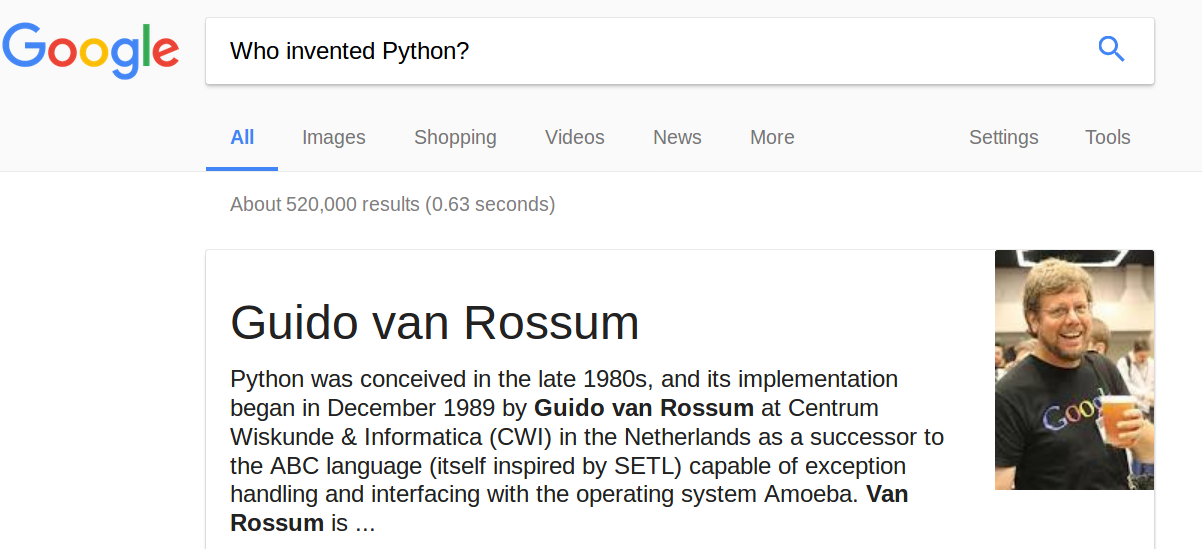
\includegraphics[width=1\linewidth]{image2/Chapitre1/guido_google.png}
	\end{minipage}
	\column{0.5\textwidth}
	\begin{minipage}[c][0.5\textheight][c]{\linewidth}
	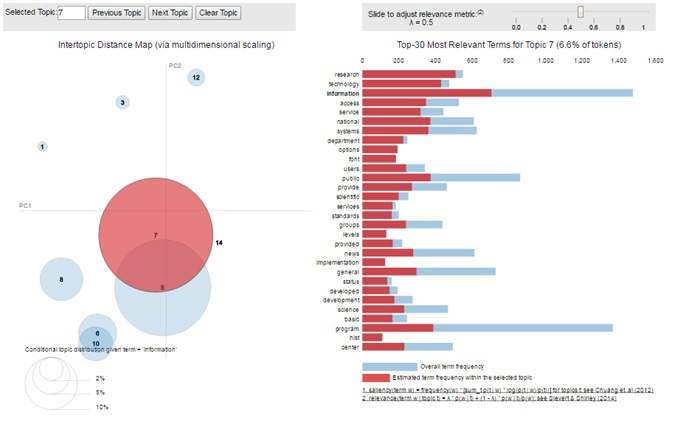
\includegraphics[width=1\linewidth]{image2/Chapitre1/lda_2d.jpg}
	\end{minipage}
	\end{columns}
	\vspace{\textheight}
\end{frame}

\begin{frame}{How do we extract meaning from text?}
%\vspace{1cm}

\begin{itemize}
\item[] {{We use \textbf{Natural Language Processing} (NLP), a field of computer science interested in making computers comprehend text and obtain useful information from it}}
\end{itemize}
\begin{figure}
\centering
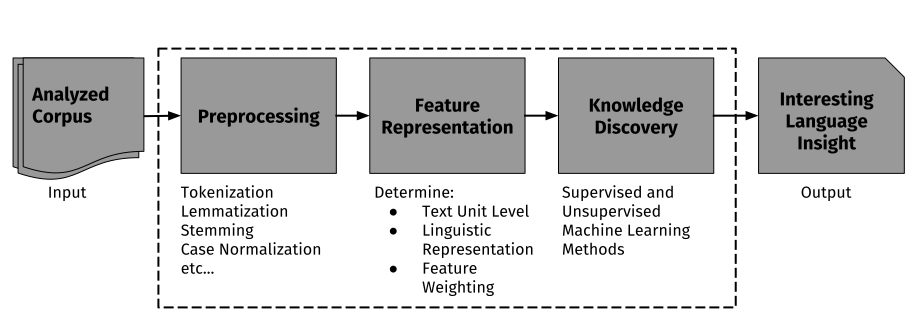
\includegraphics[width=1\linewidth]{image2/Chapitre1/nlp_flow}
\end{figure}
\vspace{\textheight}
\end{frame}

	
\begin{frame}
\frametitle{Feature Representation and Knowledge Discovery}
%\vspace{1cm}


\begin{columns}
	\column{0.5\textwidth}
	\begin{itemize}
		\item[] How do we represent text for the machine to understand? 
	\end{itemize}
	\begin{minipage}[c][0.5\textheight][c]{\linewidth}
		\centering
		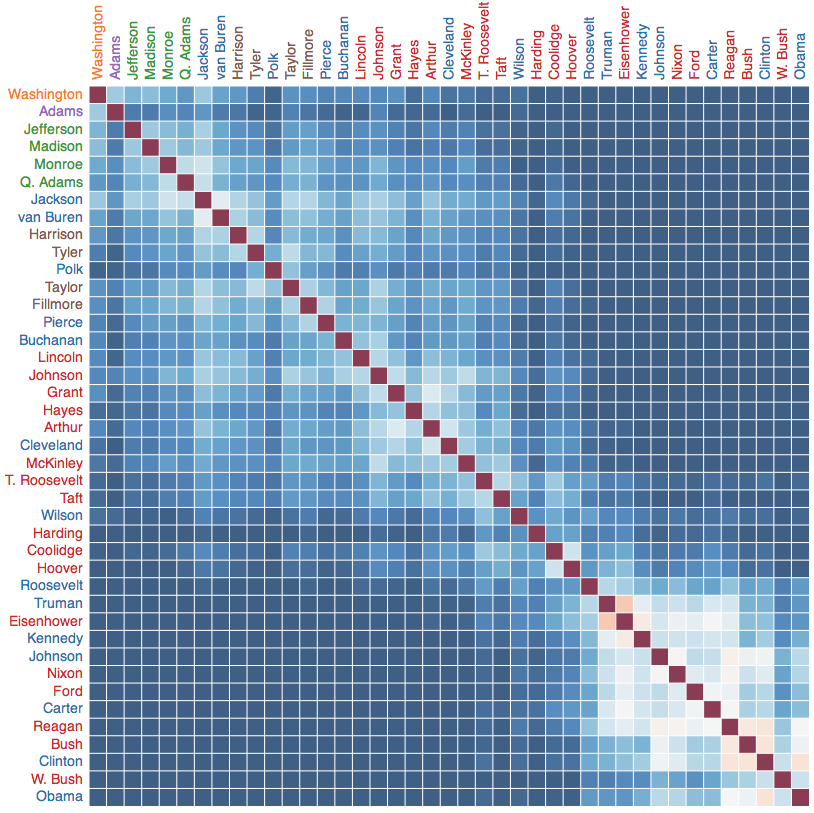
\includegraphics[width=.7\linewidth]{image2/Chapitre1/matrix.png}
	\end{minipage}
	\begin{itemize}
		\item[] Dealing with \textcolor{orangeEric}{data sparsity}
		\item[] Leveraging \textcolor{orangeEric}{heterogeneity}
	\end{itemize}	
	\column{0.5\textwidth}
	\begin{itemize}
		\item[] What techniques do we use to discover meaning from text?
	\end{itemize}
	
	\begin{minipage}[c][0.5\textheight][c]{\linewidth}
		\centering
		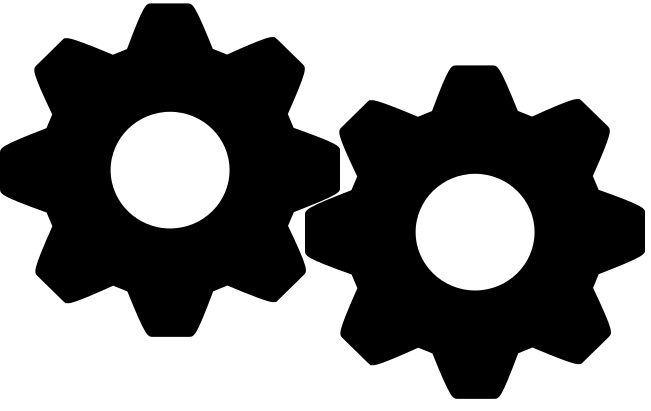
\includegraphics[width=.8\linewidth]{image2/Chapitre1/kdisc.png}

	\begin{itemize}
		\item[] Finding \textcolor{orangeEric}{semantic communities}
	\end{itemize}	
	\end{minipage}	
\end{columns}

\vspace{\textheight}

\end{frame}
%\subsection{Challenges and Contributions}

\begin{frame}{Representing Text}
%So for example, in this text, I can get features that describe its properties. They may be lexical (needing only the information of the words surrounding each word), syntactical (exaplin syntactic vs dependency tree)

\begin{itemize}
	\item \textbf{Common ways to represent text}
	\begin{itemize}
		\item Lexical
		\item Syntactic
		\begin{itemize}
				\item Constituency Tree
				\item Dependency Tree
		\end{itemize}
	\end{itemize}
	\onslide<2-> \item \textbf{Example Phrase}
	\begin{itemize}
		\item[] \textit{The report contains copies of the minutes of these meetings}
	\end{itemize}
\end{itemize}

\begin{overprint}
  				
  \onslide<3>
	  \vfill
	  \centering	  
      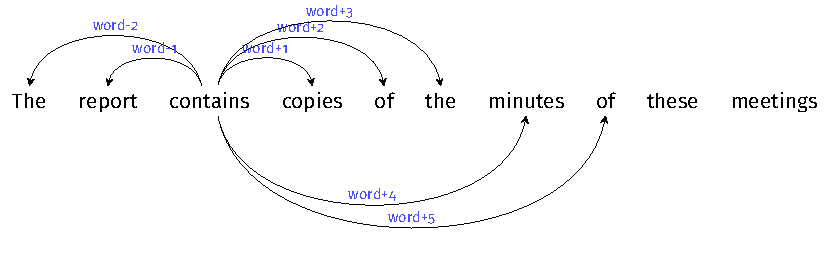
\includegraphics[width=.8\linewidth]{img/tree/lexical_tree.pdf}
	  \vfill
  \onslide<4>
	  \vfill
  	  \centering
      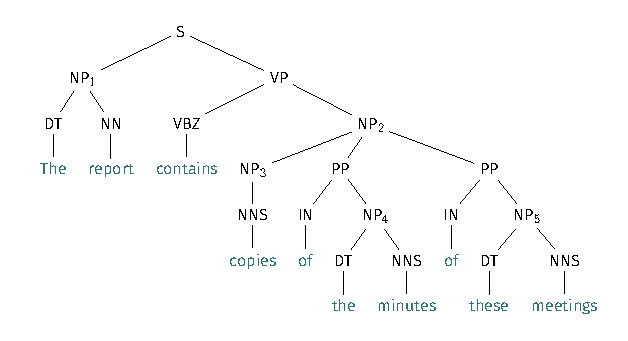
\includegraphics[width=.8\linewidth]{img/tree/tree.pdf}
      \vfill
  \onslide<5>
	  \vfill
	  \centering
      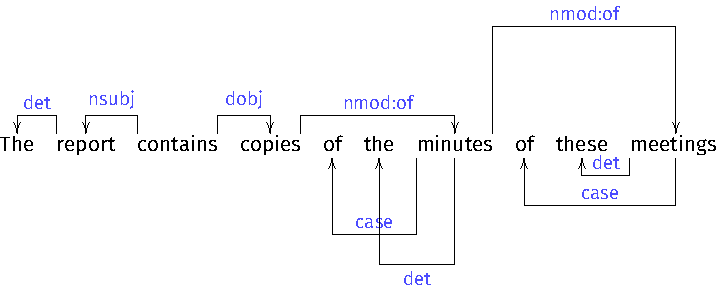
\includegraphics[width=.8\linewidth]{img/tree/dep_tree.pdf}
      \vfill
\end{overprint}
\end{frame}

\begin{frame}{Represention Models}
\begin{itemize}
\item \textbf{Two classic models}
	\begin{itemize}
		\item Graph-based 
		\item Matrix-based
	\end{itemize}
\item \textbf{Leveraging the network structure}
	\begin{itemize}
		\item We can find communities of similiar words according to their meaning
	\end{itemize}
\end{itemize}
\begin{overprint}
	  % on every slide (not sure if it is officially supported)
	  \onslide<2>
	  \centering
	      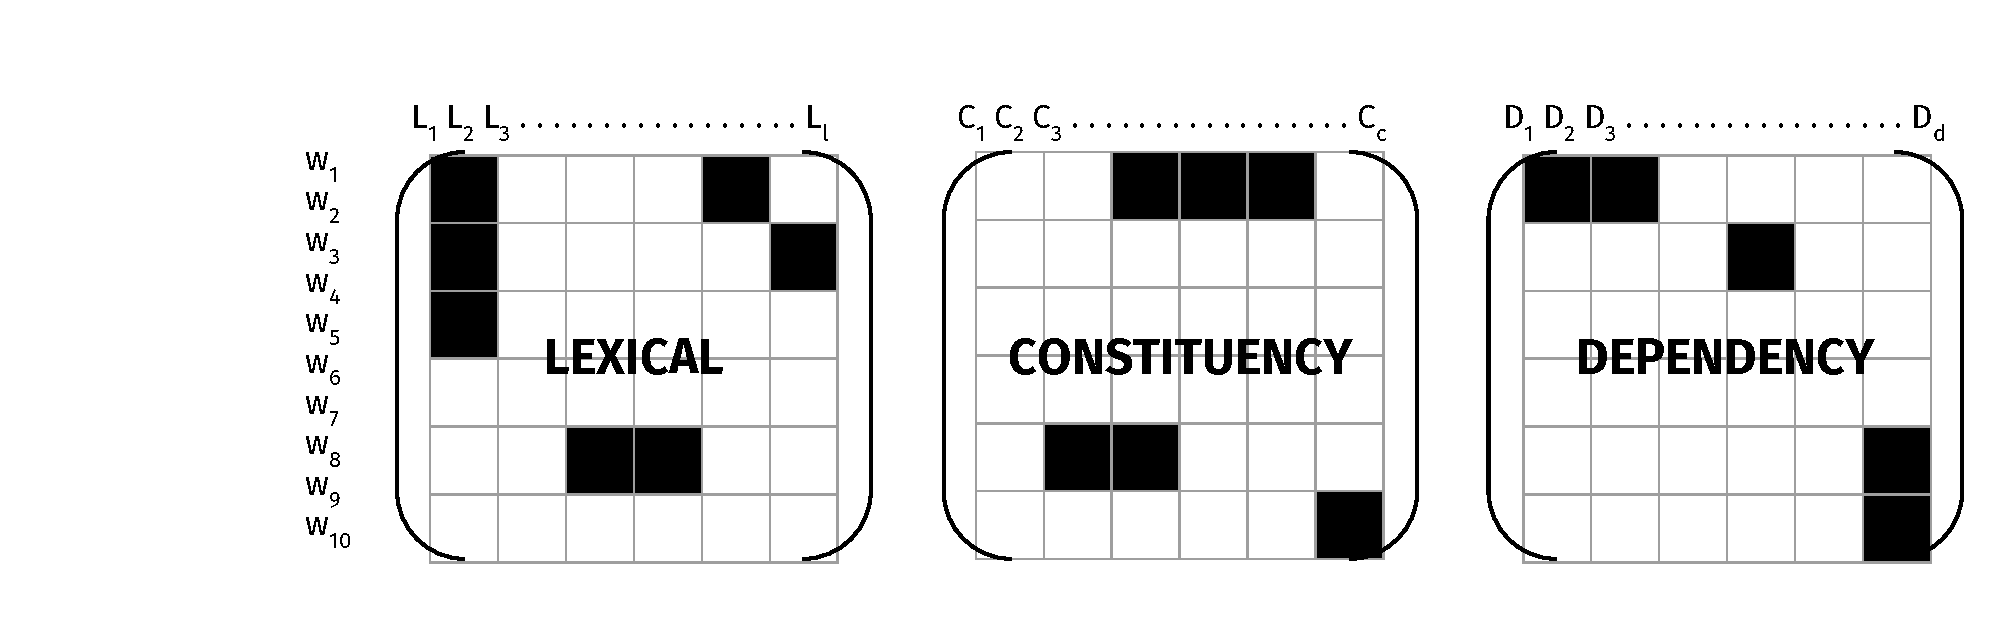
\includegraphics[width=.8\linewidth]{image2/Chapitre1/feature_types.pdf}	
%	  \onslide<3>
%	  \centering
%		  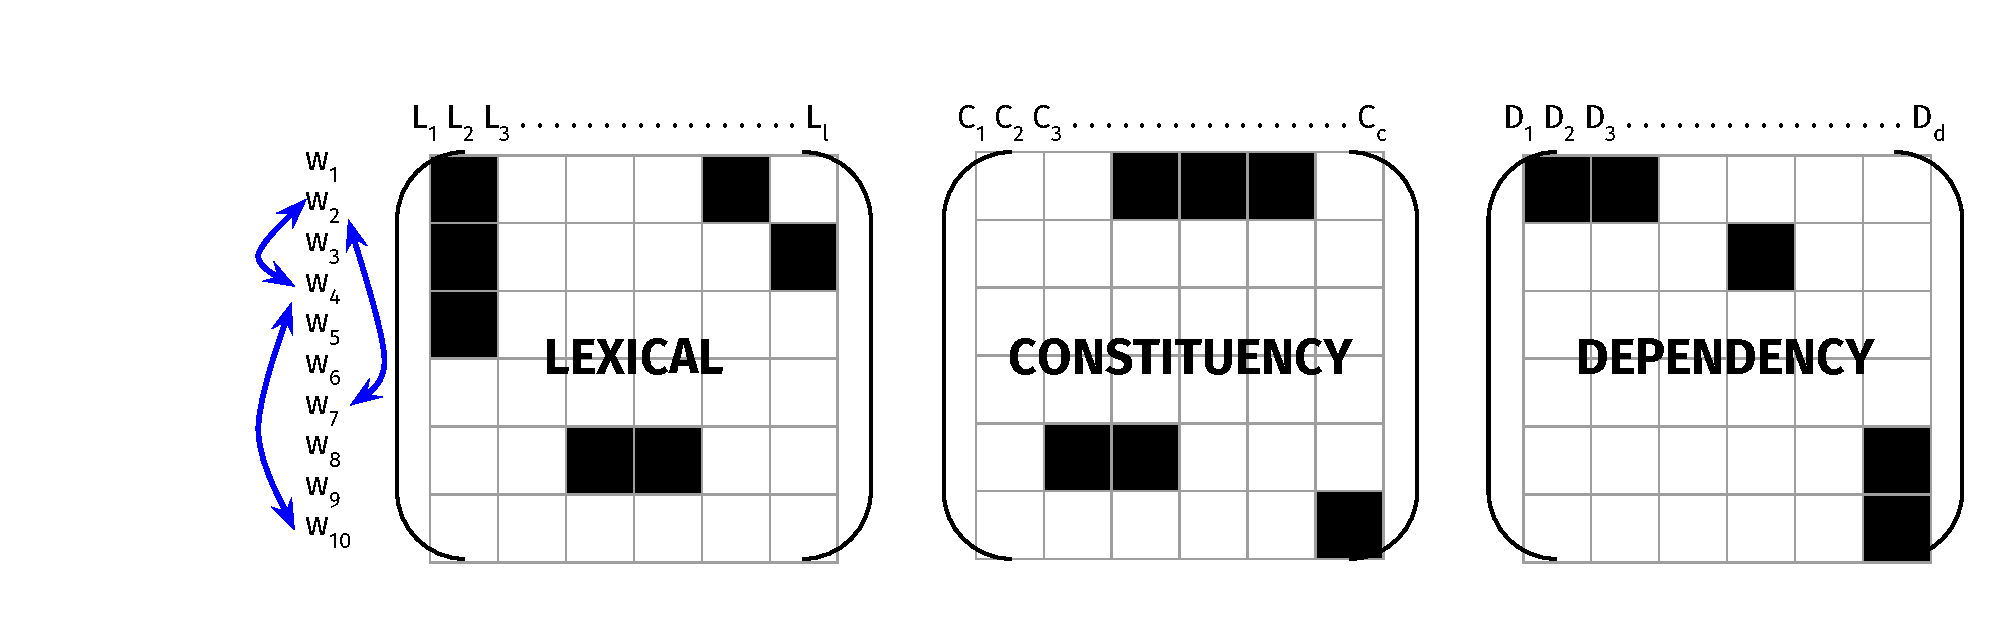
\includegraphics[width=\linewidth]{image2/Chapitre1/feature_types_communities.pdf}	  
	  % on slide two
\end{overprint}

\end{frame}


\begin{frame}{Main Challenges and Contributions}
\vspace{1cm}
	\begin{enumerate}
		\item<1-> What type of model can we employ to represent a corpus  \textcolor{orangeEric}{using heterogeneous features}?
		\begin{itemize}
		\item<1-> \textit{Hypergraph model to  \textcolor{greenEric}{hold different types of  linguistic information}}
		\end{itemize}
		
		\item<2-> How can we combine these features while  \textcolor{orangeEric}{dealing with feature sparsity}?
		\begin{itemize}
		\item<2-> \textit{Multimedia fusion techniques to \textcolor{greenEric}{combine and densify} representation spaces}	    	 
		\end{itemize}
		\item<3-> How can we \textcolor{orangeEric}{find communities} existing within the language networks?
		\begin{itemize}
		\item<3-> \textit{An alternative network-based algorithm to \textcolor{greenEric}{discover semantically related words} within a text}
		\end{itemize}
		
	\end{enumerate}
 \vspace{\textheight}
\end{frame}


\begin{frame}{Work Overview}
\begin{center}
\vfill
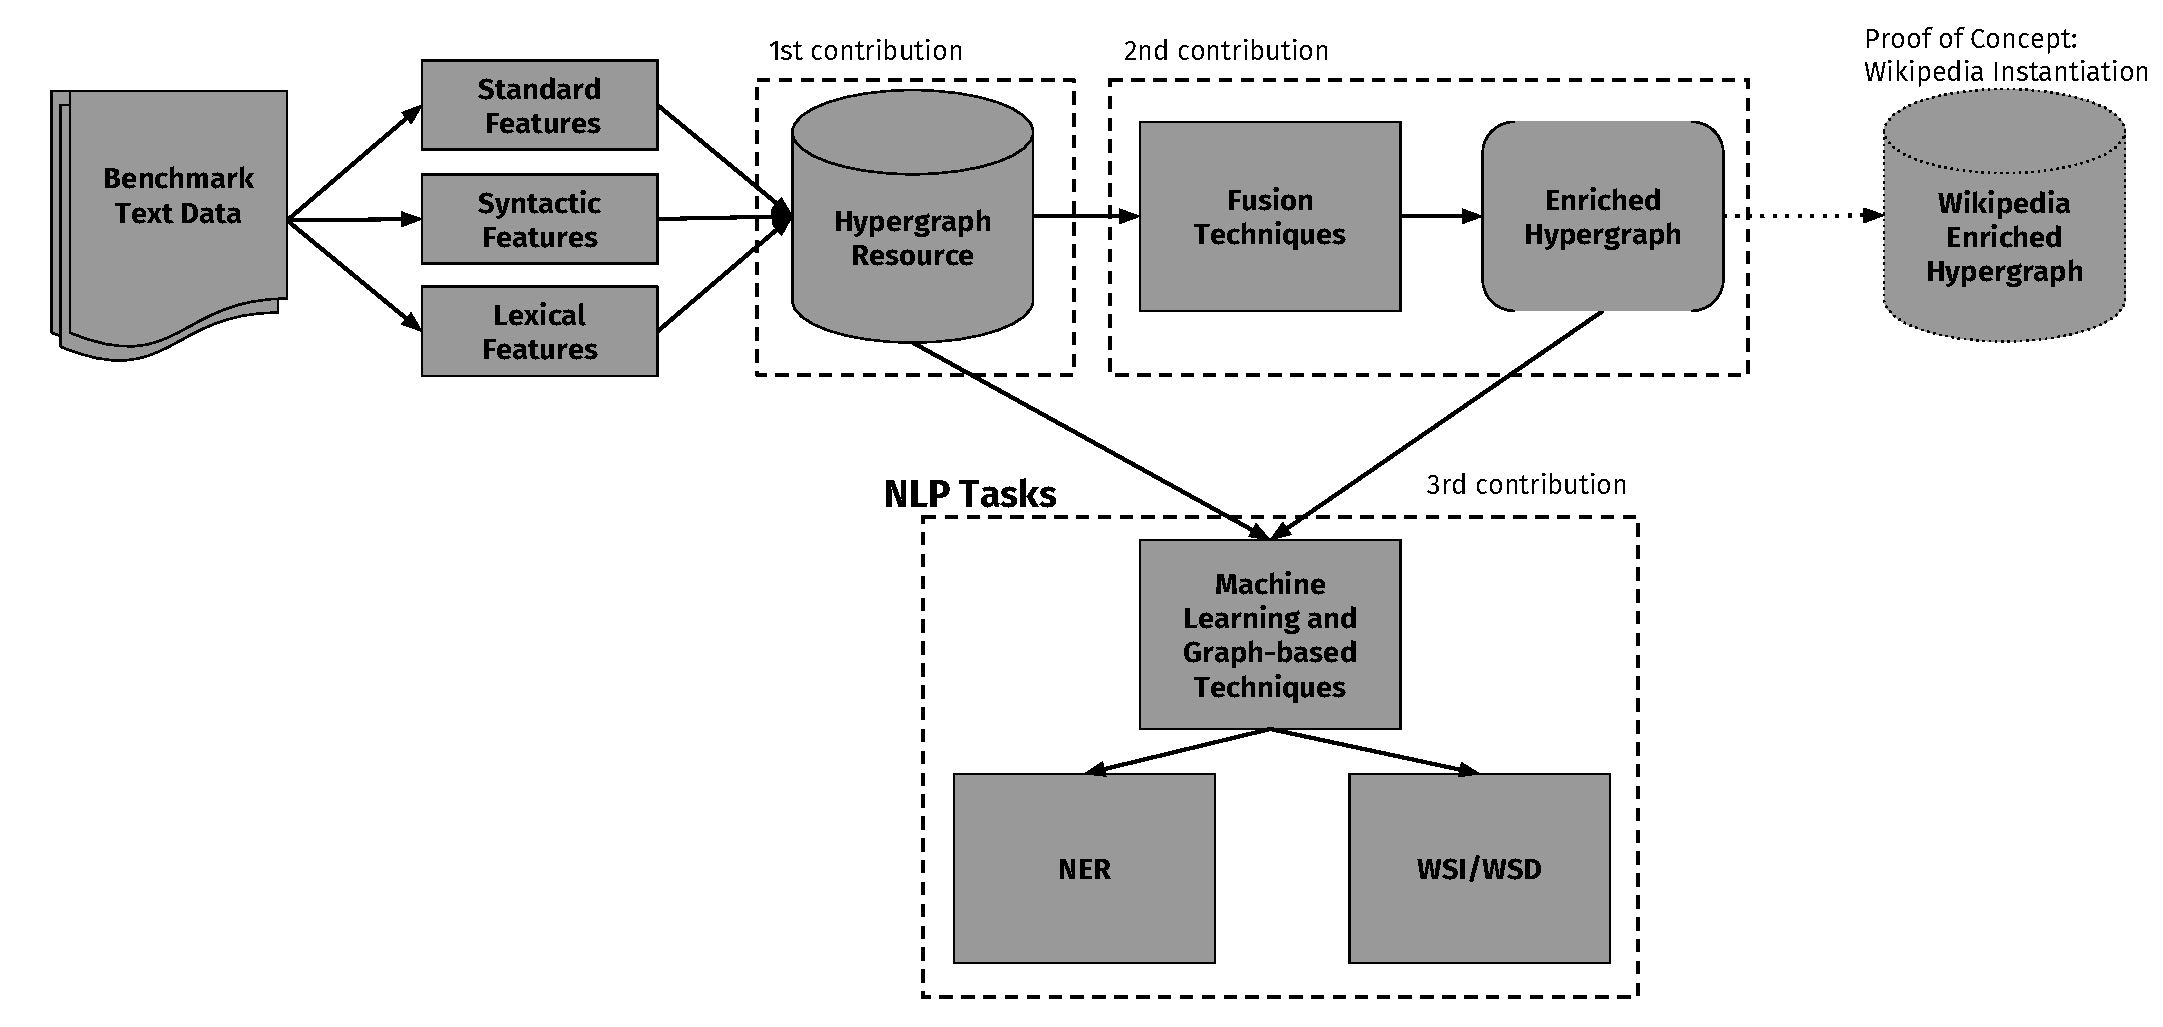
\includegraphics[width=1.04\linewidth]{image2/Chapitre1/main_diag_presi.pdf}
\end{center}
\vfill
% \vspace{\textheight}
\end{frame}

\setbeamertemplate{section page}[mytheme][image2/Chapitre1/main_diag_presi.pdf]

\section[Contributions in Detail]{Hypergraph Linguistic Model}
\metroset{sectionpage=none}
\section{Hypergraph Linguistic Model}
\metroset{sectionpage=simple}
%\begin{frame}{Work Overview}
%%\large  \textbf{Approach Overview} \hfill
%\begin{center}
%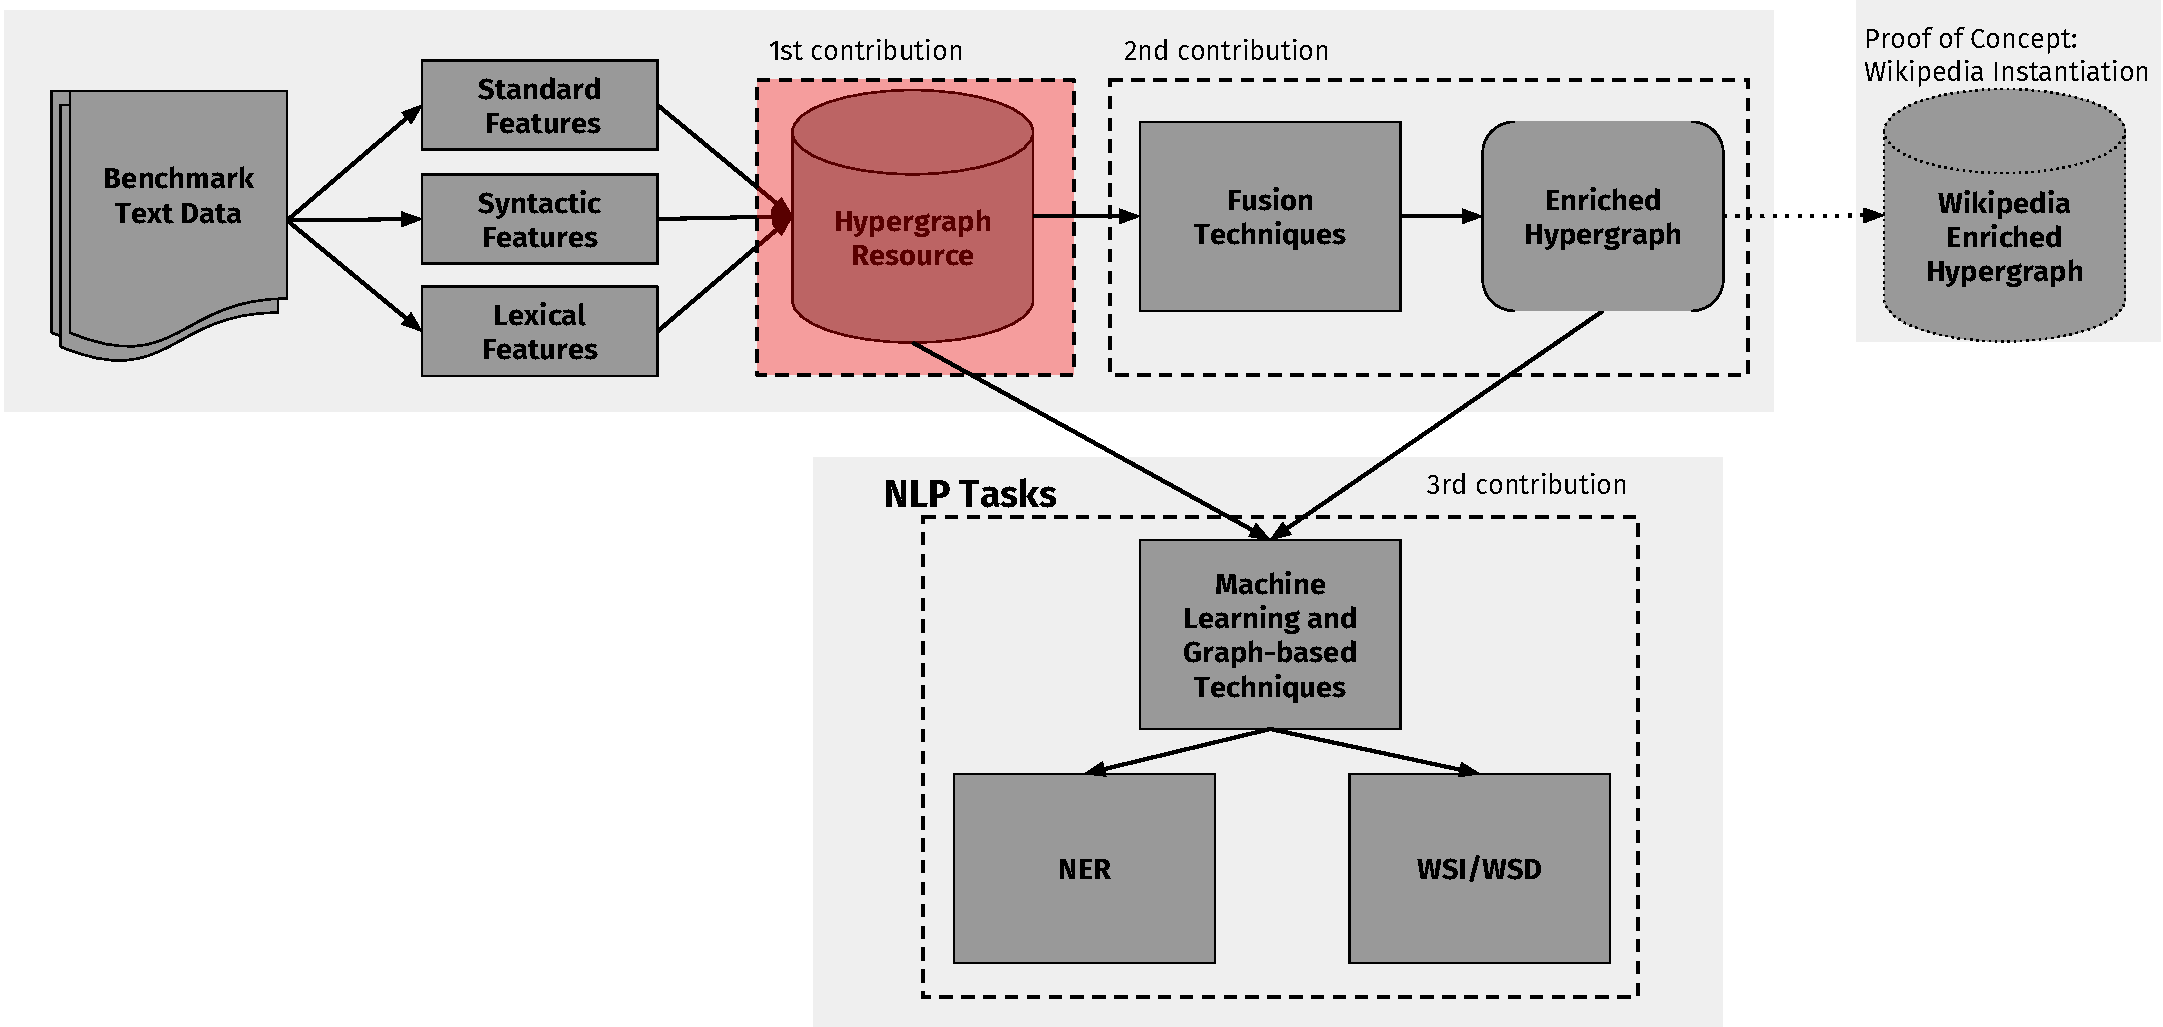
\includegraphics[width=1.04\linewidth]{image2/Chapitre3/main_diag_contr1.pdf}
%\end{center}
%
% \vspace{\textheight}
%\end{frame} 


\begin{frame}{Introduction}

We extract useful information from a text based on the \textcolor{orangeEric}{distributional hypothesis} (a word is defined by its surroundings) 
\begin{itemize}
	\item \textbf{We choose network models} 
		\begin{itemize}
		\item Used in a large quantity of NLP tasks 
		\item Graphs structures can give us a clearer view into the relations of words within a text 	
		\item Ultimately graphs are transformed to a vectorial representation through the adjacency/incidence matrices
		
		\end{itemize}
		
\end{itemize}
\vspace{\textheight}
\end{frame}




\begin{frame}{Classic Language Networks}
%What is the state of the art ? How is text is represented by means of networks?
% Three main types
%todo Add here the networks by choudhury et al venus stuff

\begin{itemize}
\item[] \large \textbf{Example phrase}
\item[] \textit{The report contains copies of the minutes of these meetings} 
\end{itemize}

\begin{overprint}
  % on every slide (not sure if it is officially supported)
  \onslide<2>
	  \centering
	  
	  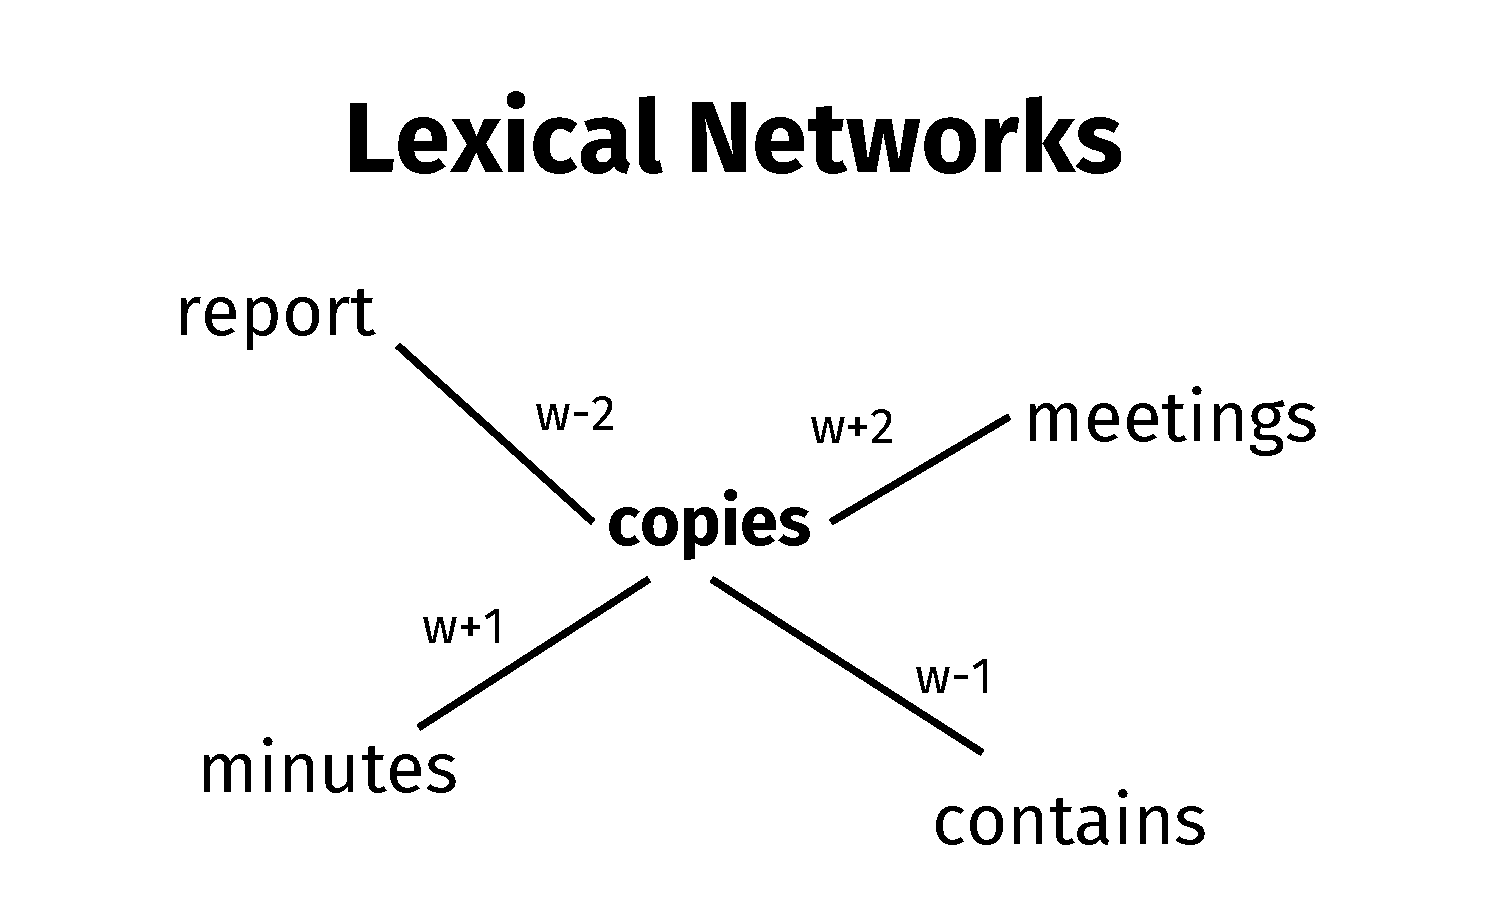
\includegraphics[width=.6\linewidth]{image2/Chapitre2/lexi_network_ex.pdf}
%	  \\ \cite{2008.Klapaftis.WSIUsingCollocations}
  \onslide<3>
	  \centering
  	  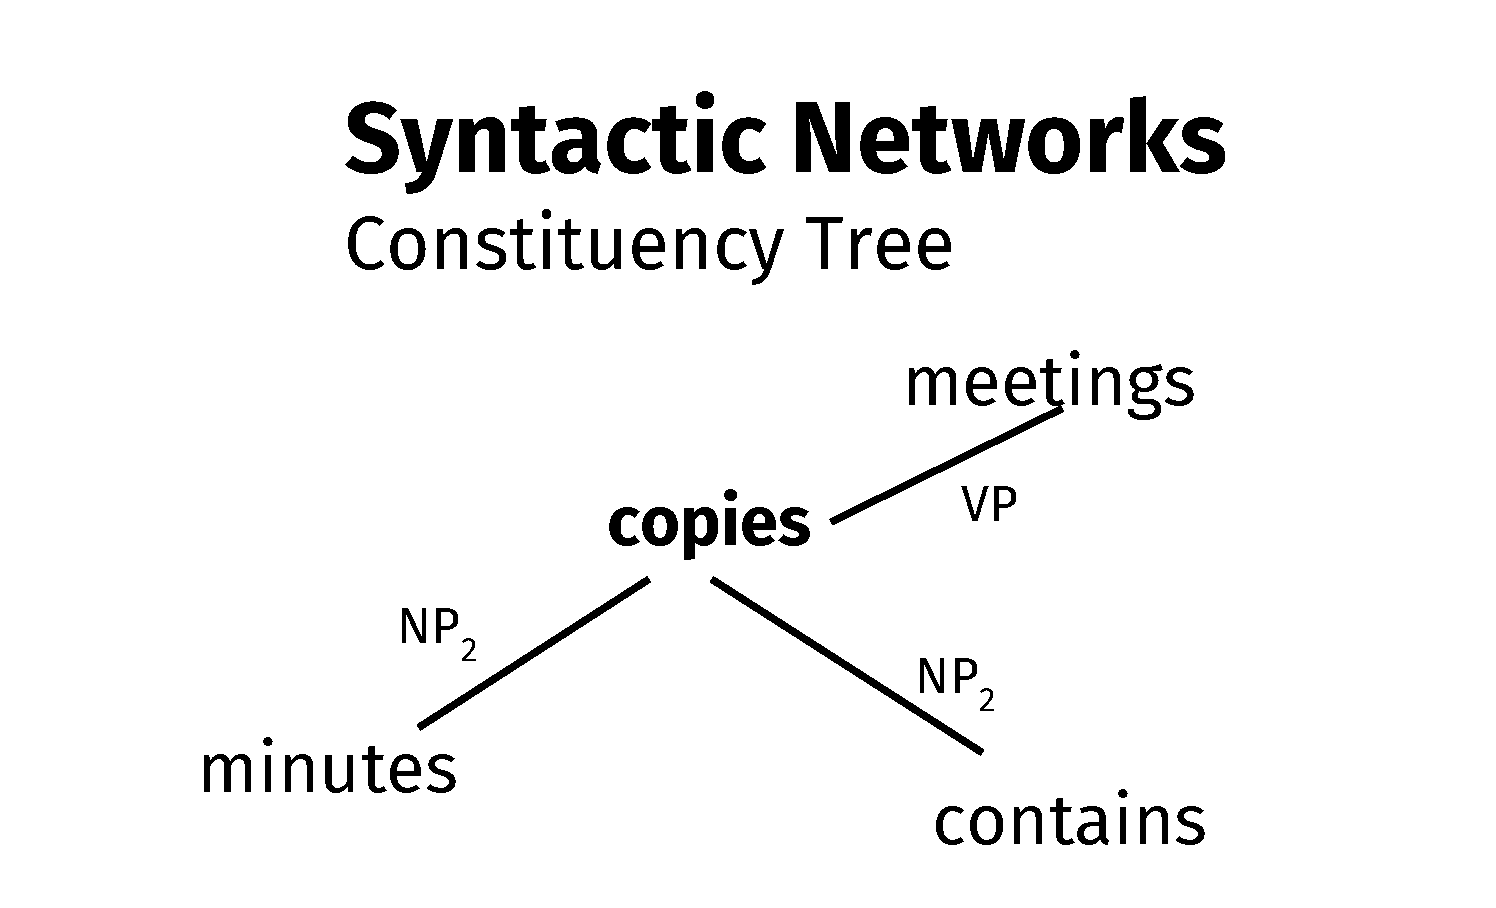
\includegraphics[width=.6\linewidth]{image2/Chapitre2/consti_network_ex.pdf}   
  \onslide<4>
	  \centering
	  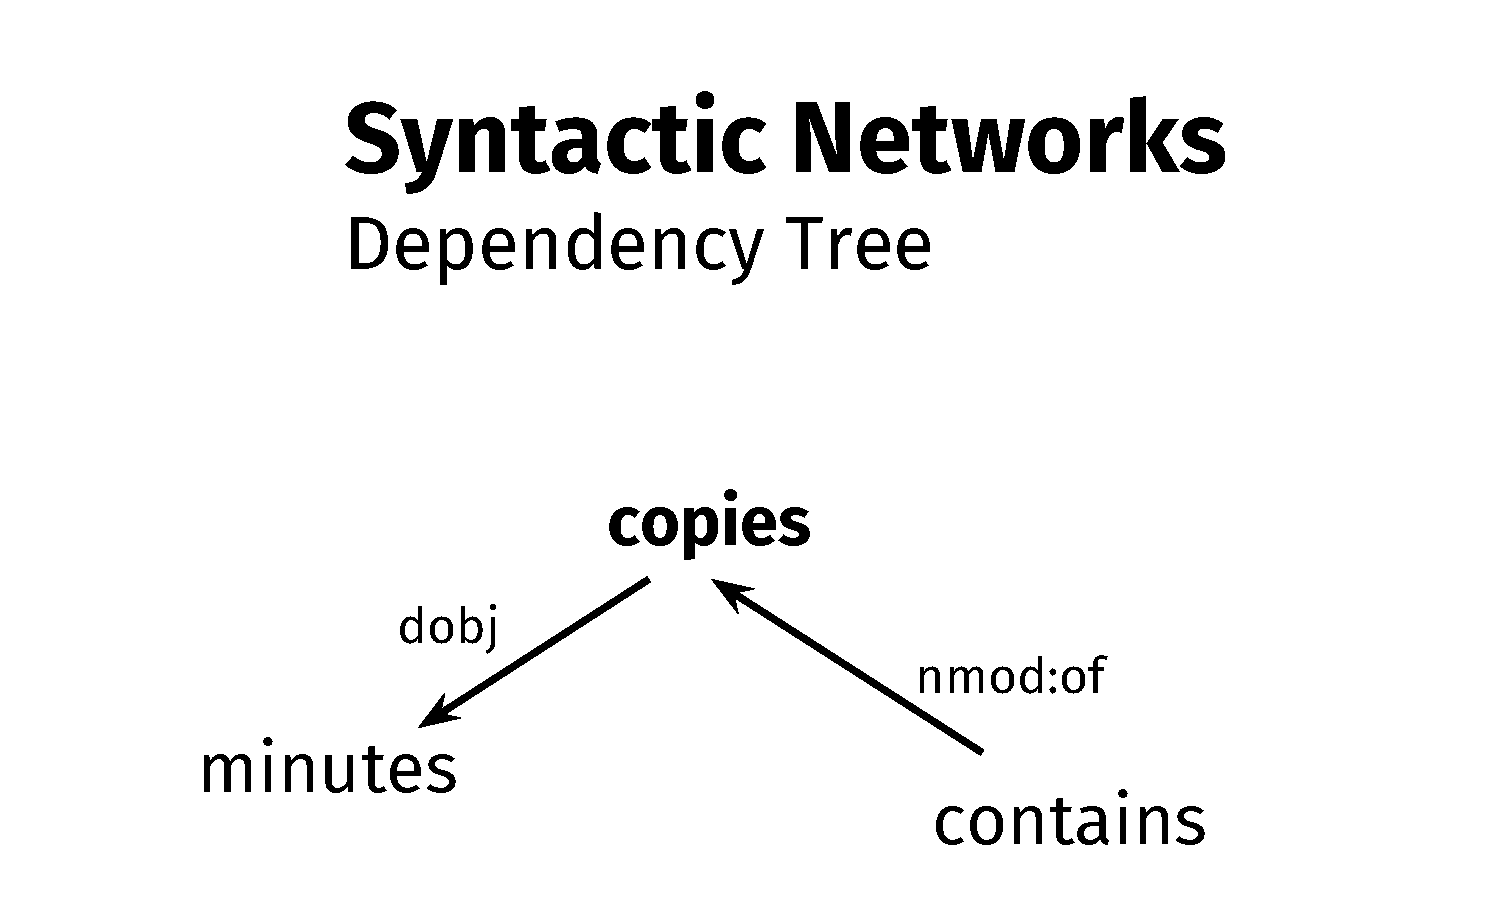
\includegraphics[width=.6\linewidth]{image2/Chapitre2/deps_network_ex.pdf} 
%  \onslide<5>
%	  \centering
%	  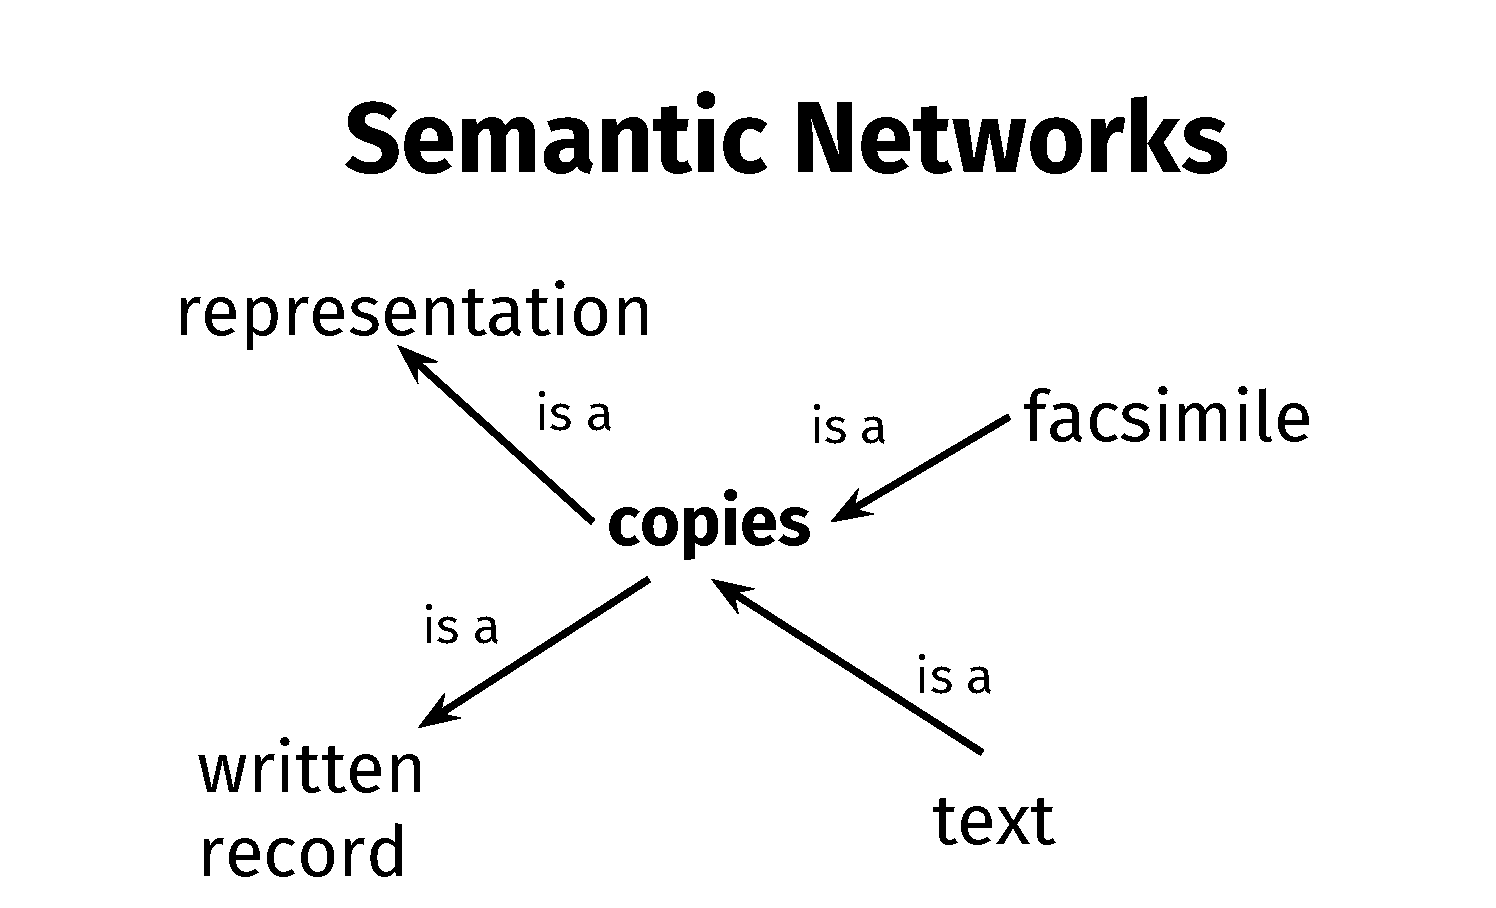
\includegraphics[width=.7\linewidth]{image2/Chapitre2/sem_network_ex.pdf}   

  % on slide three
  % etc.
\end{overprint}


\end{frame}


\begin{frame}{Limitations and Proposition}
\begin{itemize}
\item<1-> \large \textbf{Limitations of existing representations}
	\begin{itemize}
	\item<1-> Language networks generally employ a single type of textual information
	\item<1-> The edges of the network relate maximum two words at each time
	\end{itemize}
\item<2-> \large \textbf{Proposition}
	\begin{itemize}
	\item<2-> Use a hypergraph model to link together the different types of networks
	\item<2-> This allows for a semantic overview at three different layers: short range, medium range, and long range at once
	\item<2-> Relating more than two words at the same time
	\end{itemize}
\end{itemize}
\vspace{\textheight}
\end{frame}

\begin{frame}{Proposed Model}
%	\begin{itemize}
%		\item Explain (grpahically/with the working exampleh) we use lexical and syntactic info and the build a fusion of them with a hypergraph.
%	\end{itemize}
	\begin{columns}
		\column{.33\textwidth}
		\begin{minipage}[c][0.4\textheight][c]{\linewidth}
			 \centering
			 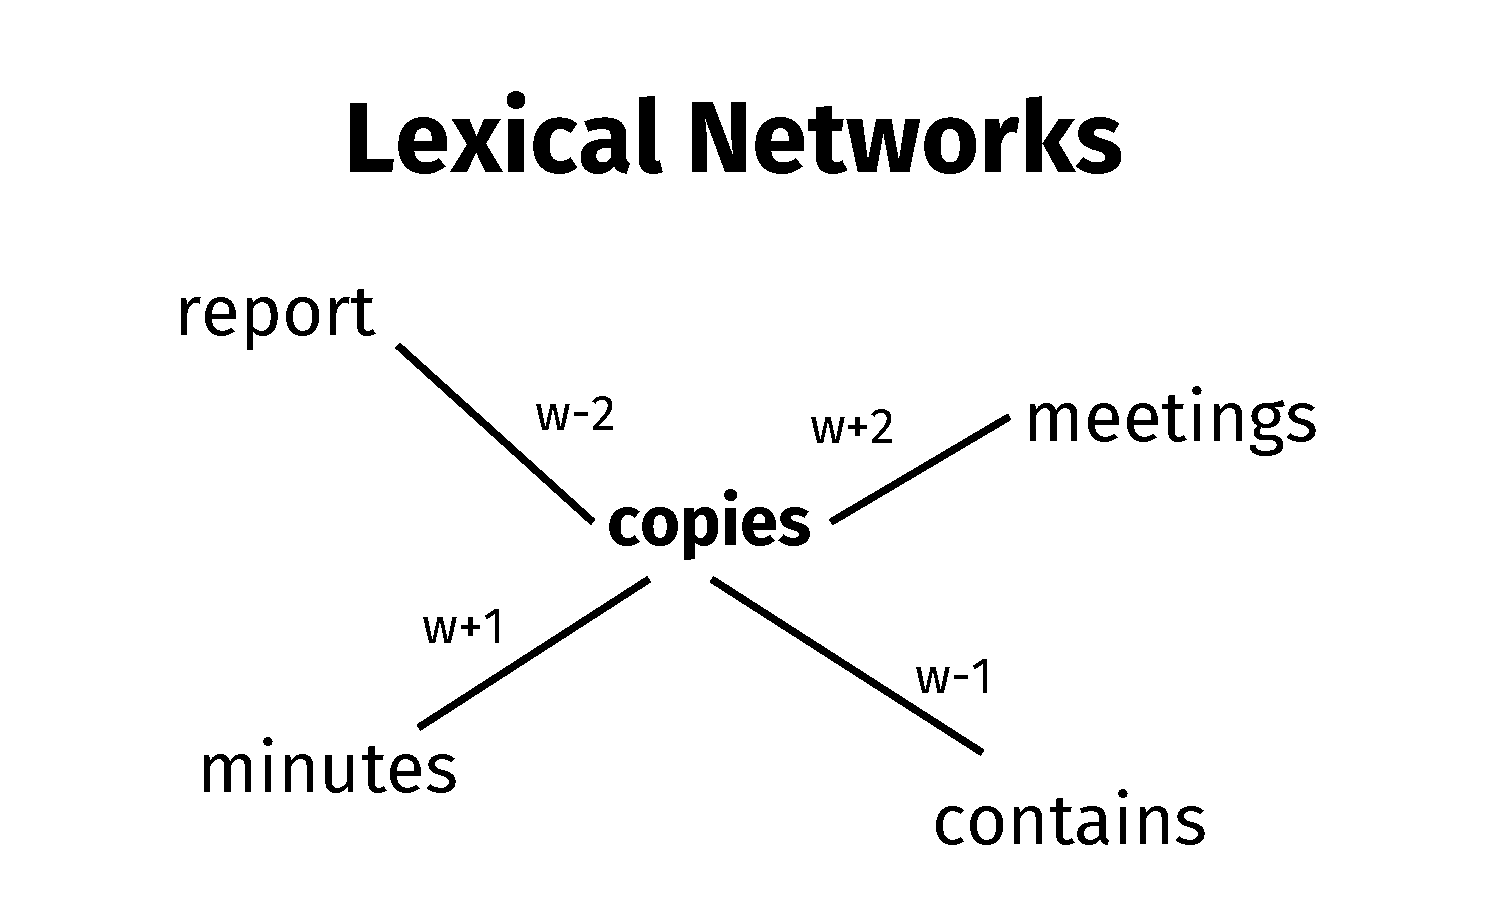
\includegraphics[width=1\linewidth]{image2/Chapitre2/lexi_network_ex.pdf}
		\end{minipage}
		\column{.33\textwidth}
		\begin{minipage}[c][0.4\textheight][c]{\linewidth}
			 \centering
			 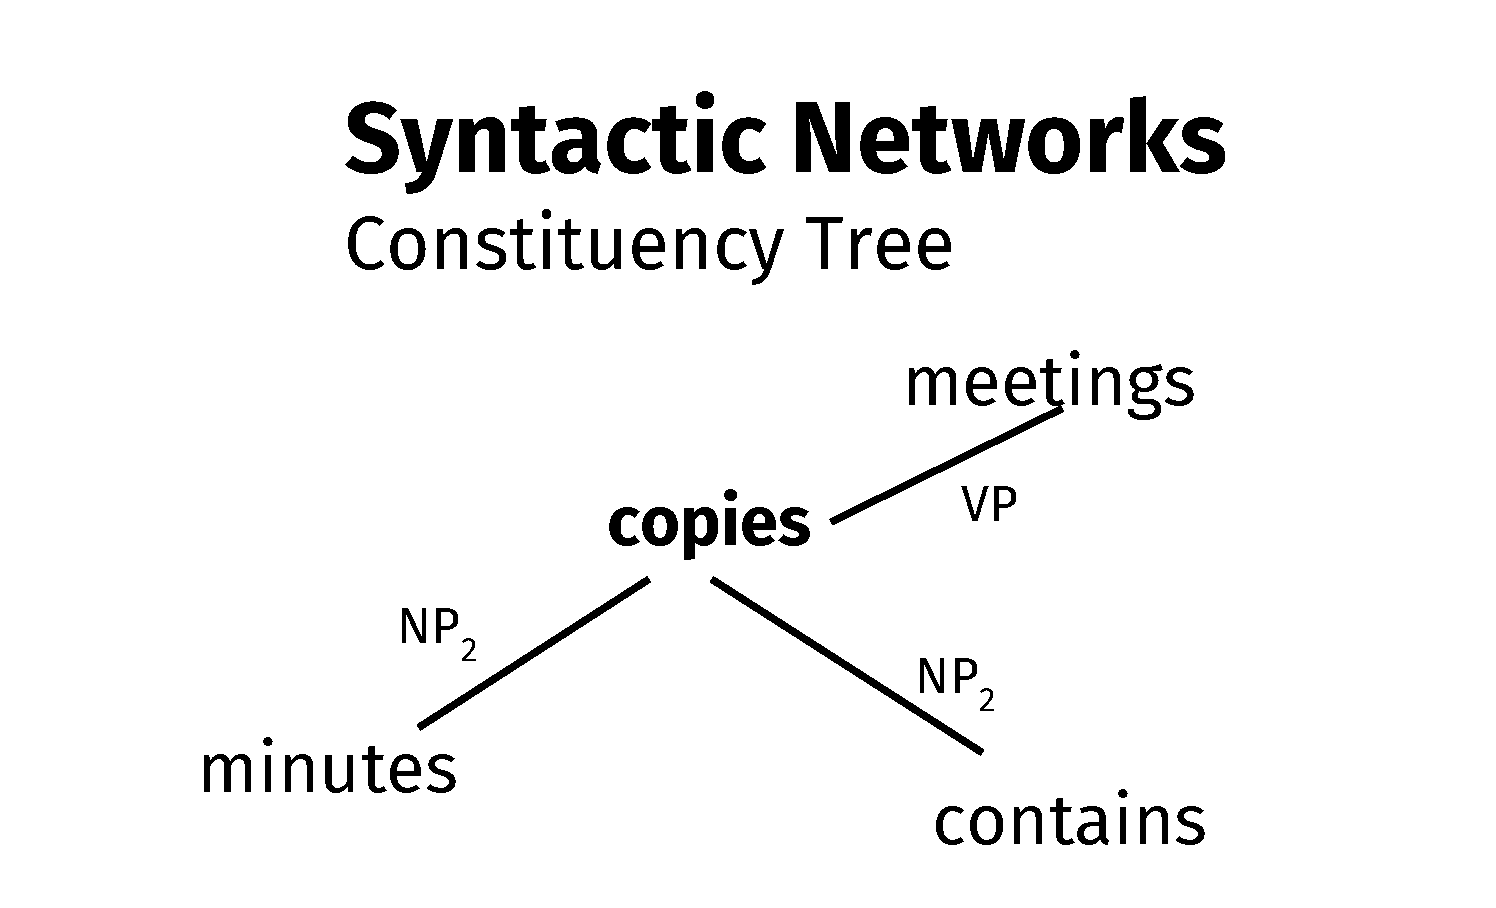
\includegraphics[width=1\linewidth]{image2/Chapitre2/consti_network_ex.pdf}
		\end{minipage}		
		\column{.33\textwidth}
		\begin{minipage}[c][0.4\textheight][c]{\linewidth}
			 \centering
				 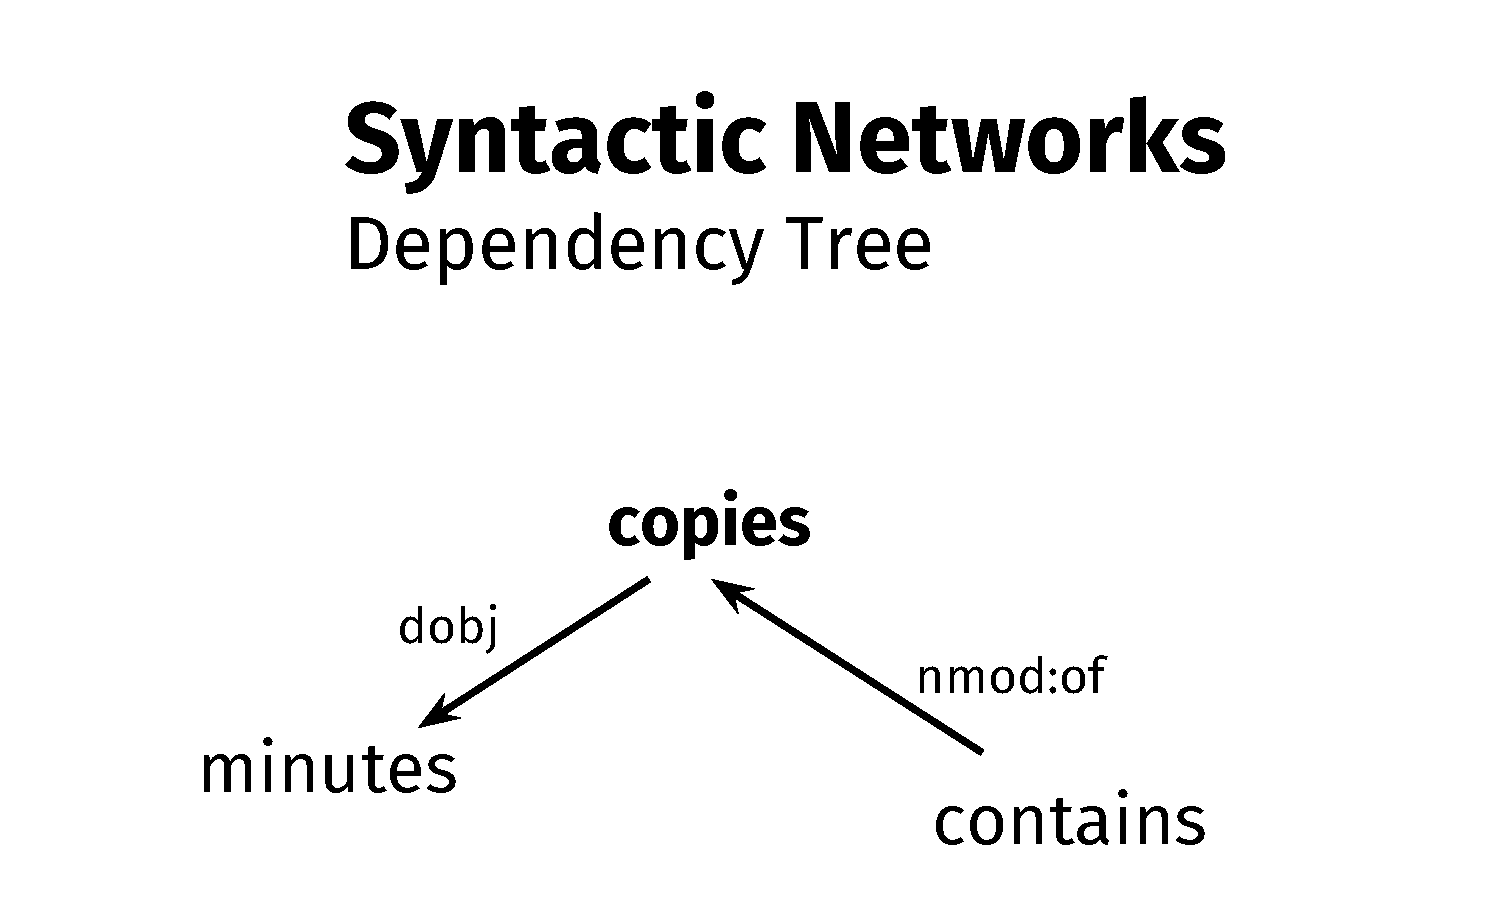
\includegraphics[width=1\linewidth]{image2/Chapitre2/deps_network_ex.pdf}
		\end{minipage}
	\end{columns}
	

	
	\begin{overprint}
	\onslide<2>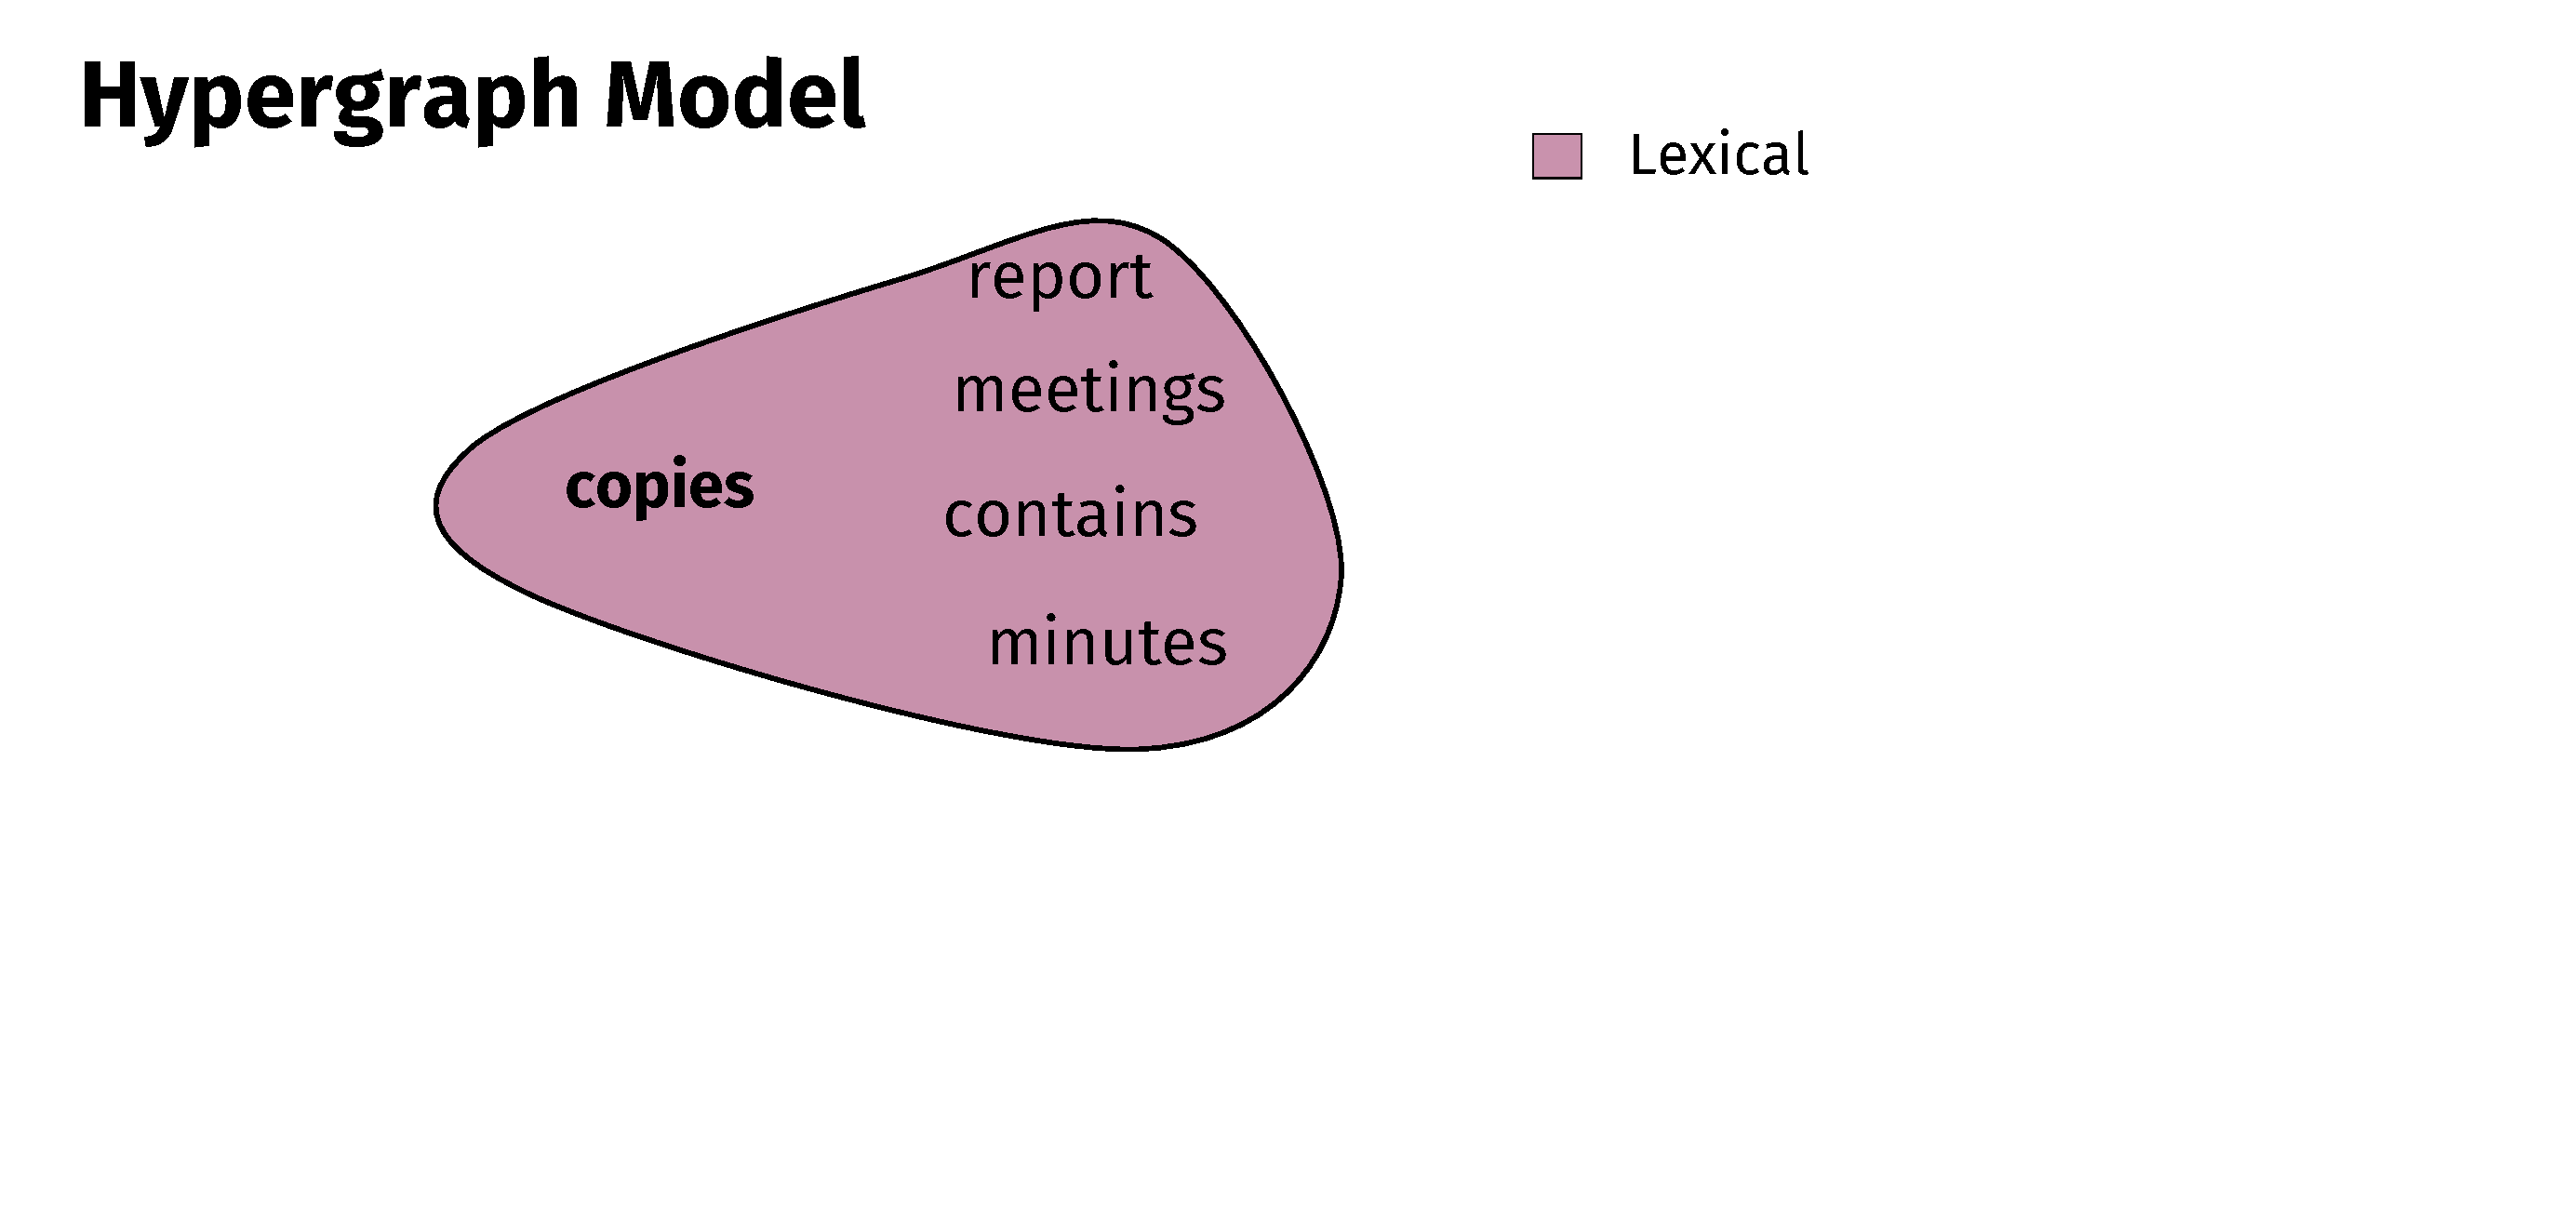
\includegraphics[width=1\linewidth]{image2/Chapitre2/hyper_network_ex_1.pdf}%lexical
	\onslide<3>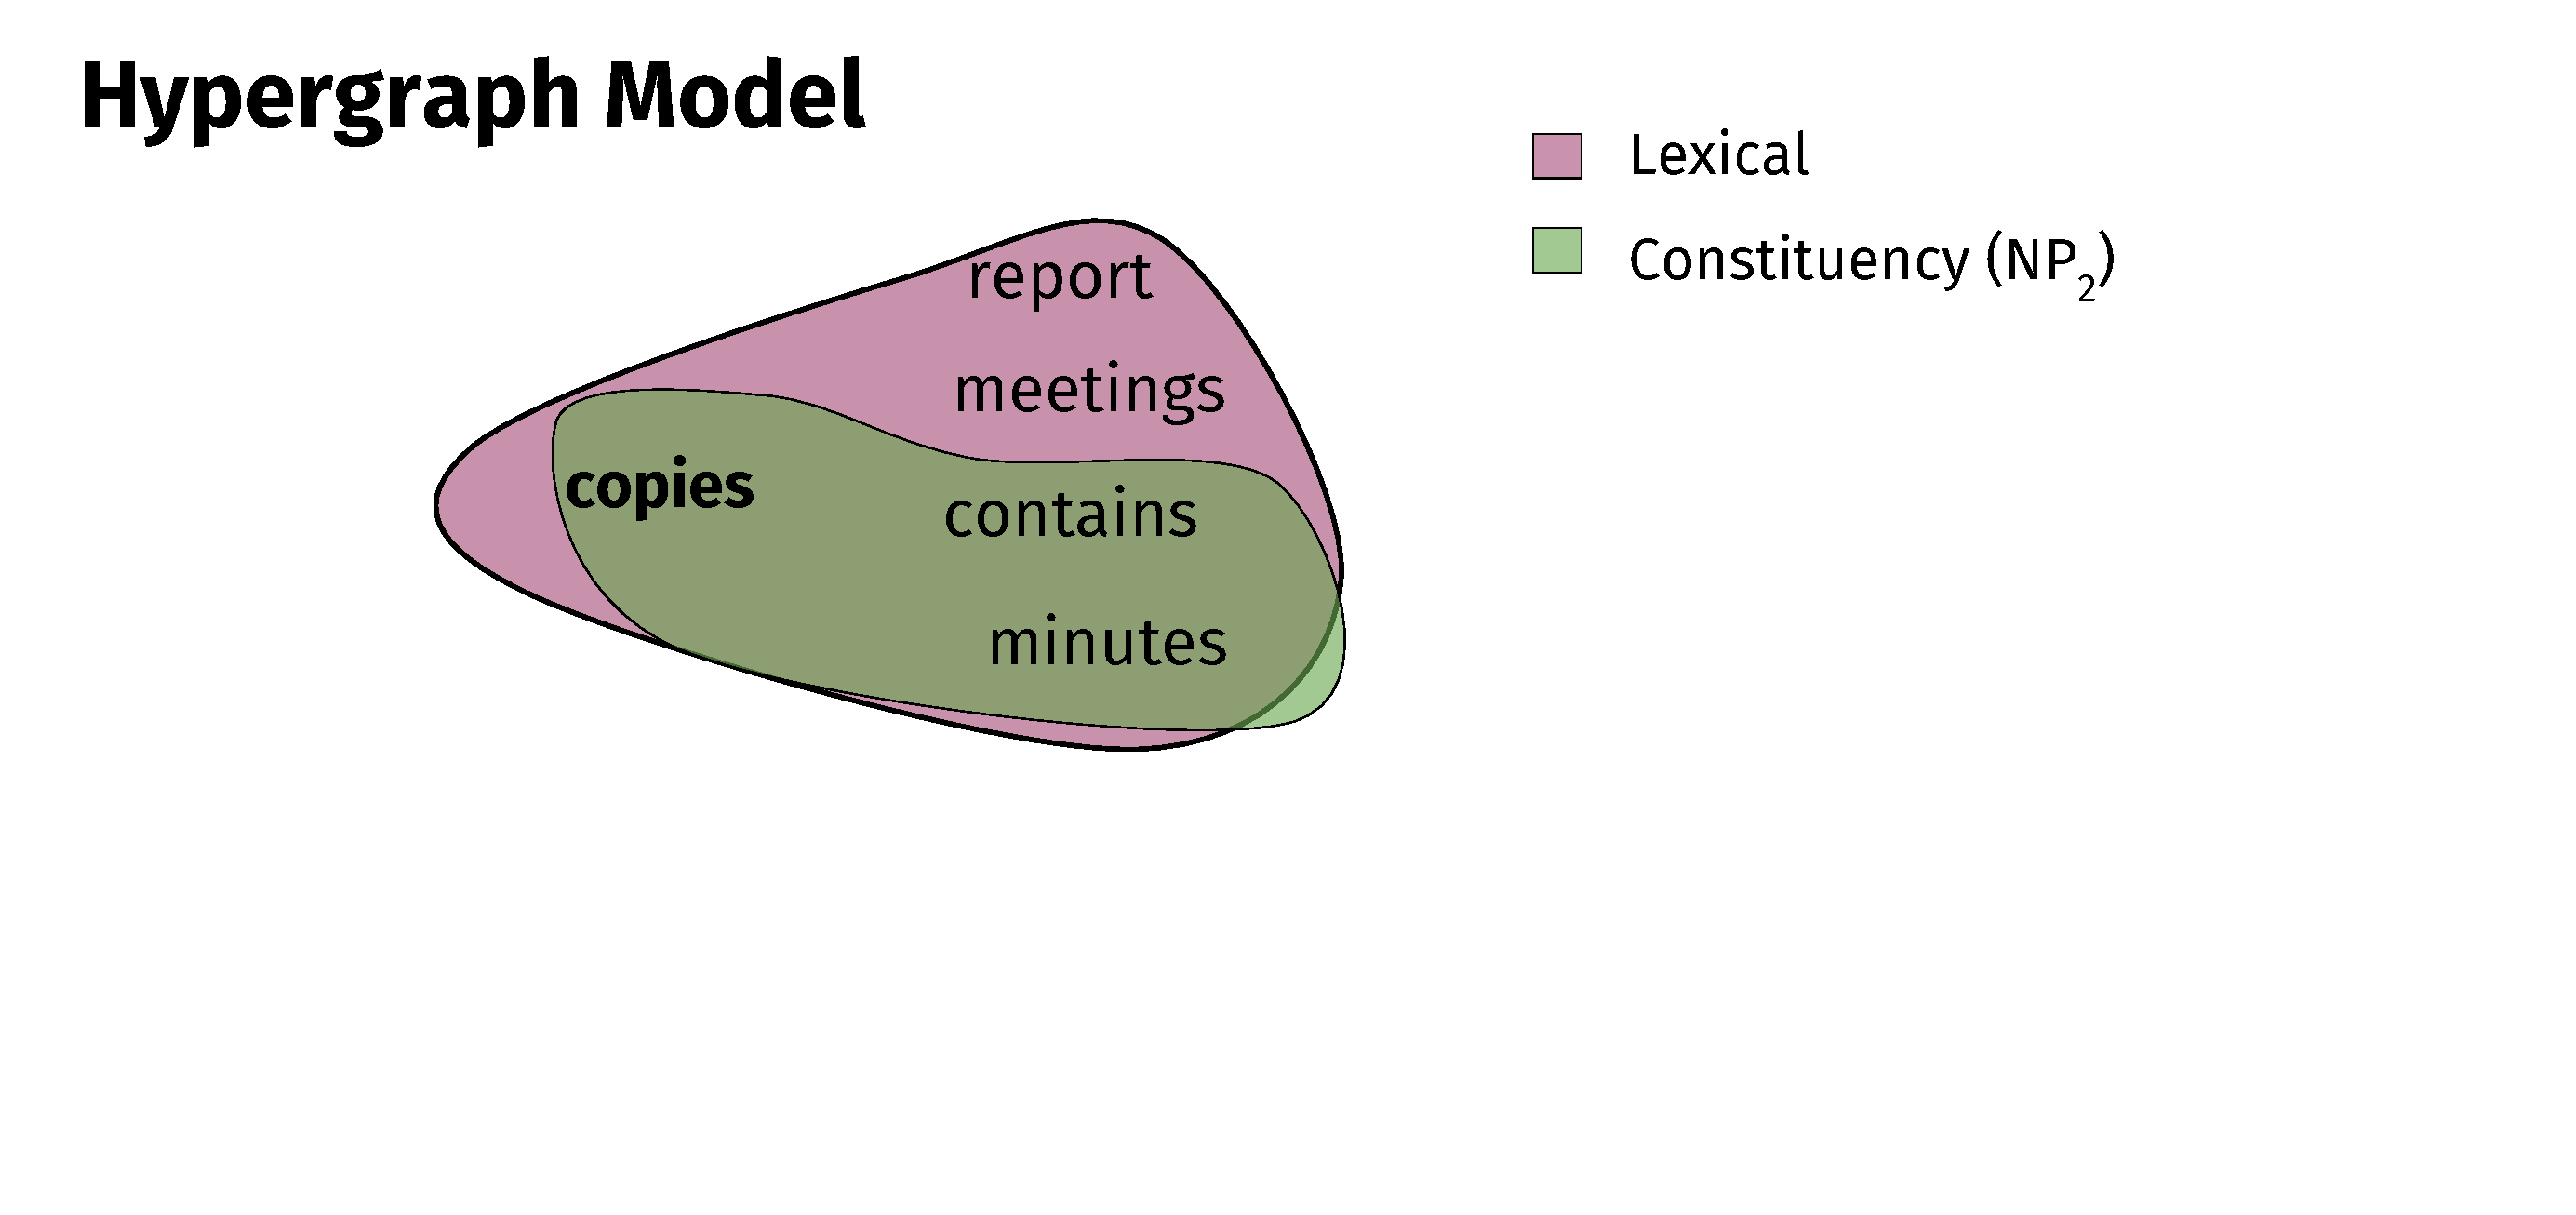
\includegraphics[width=1\linewidth]{image2/Chapitre2/hyper_network_ex_2.pdf}%constit
	\onslide<4>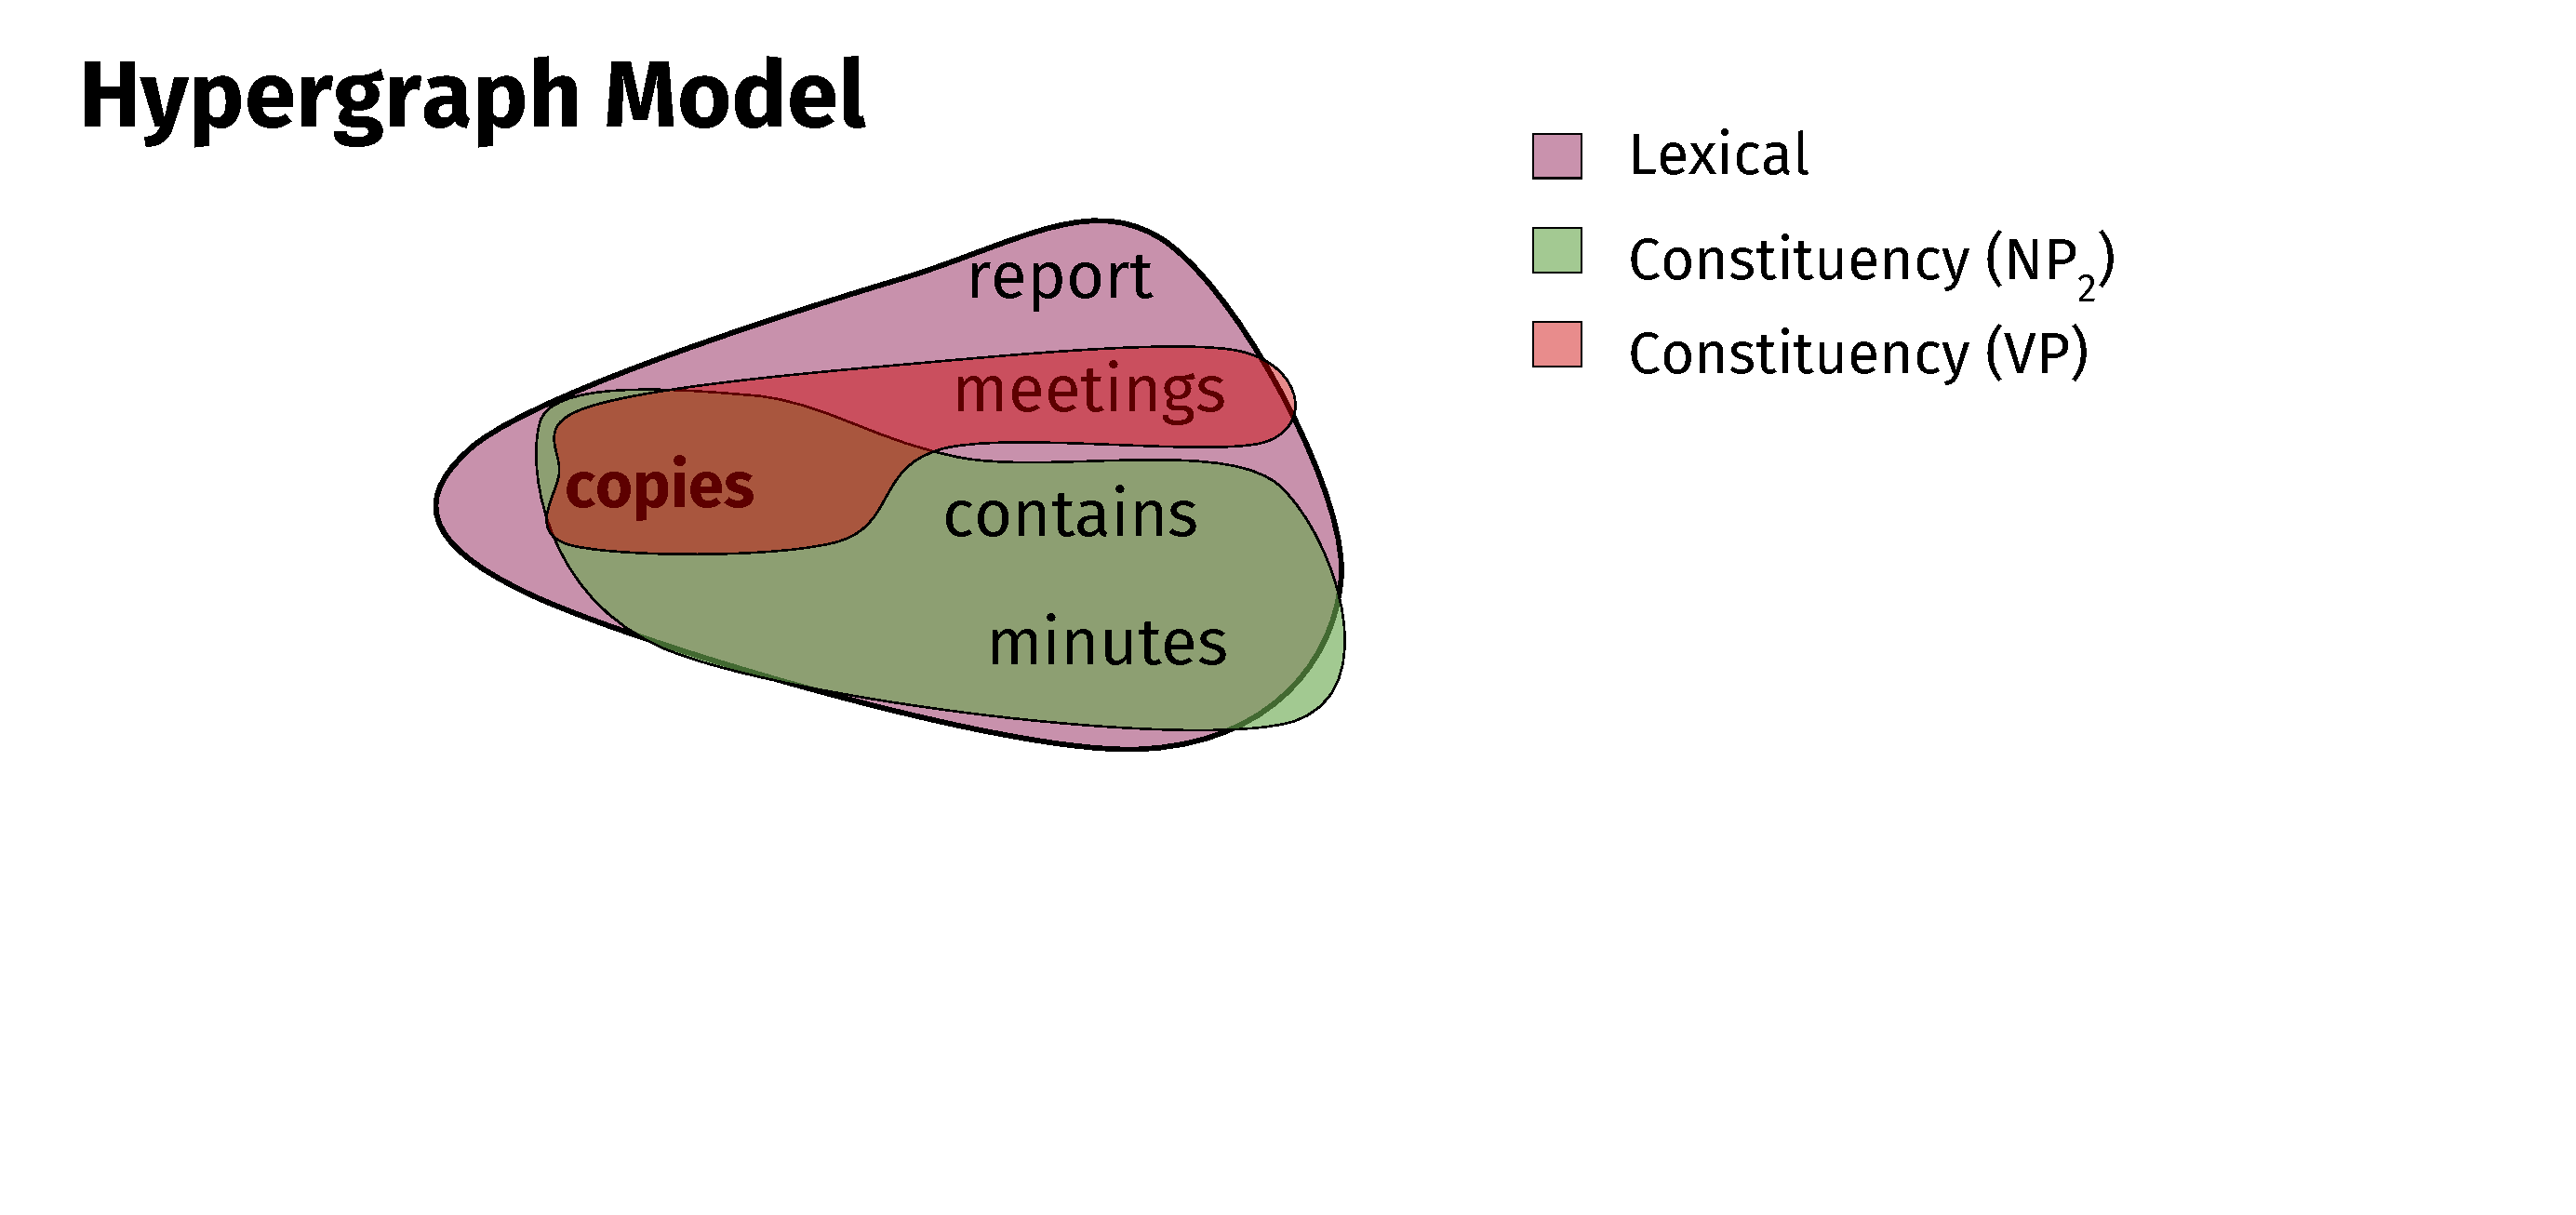
\includegraphics[width=1\linewidth]{image2/Chapitre2/hyper_network_ex_3.pdf}%constit
	\onslide<5>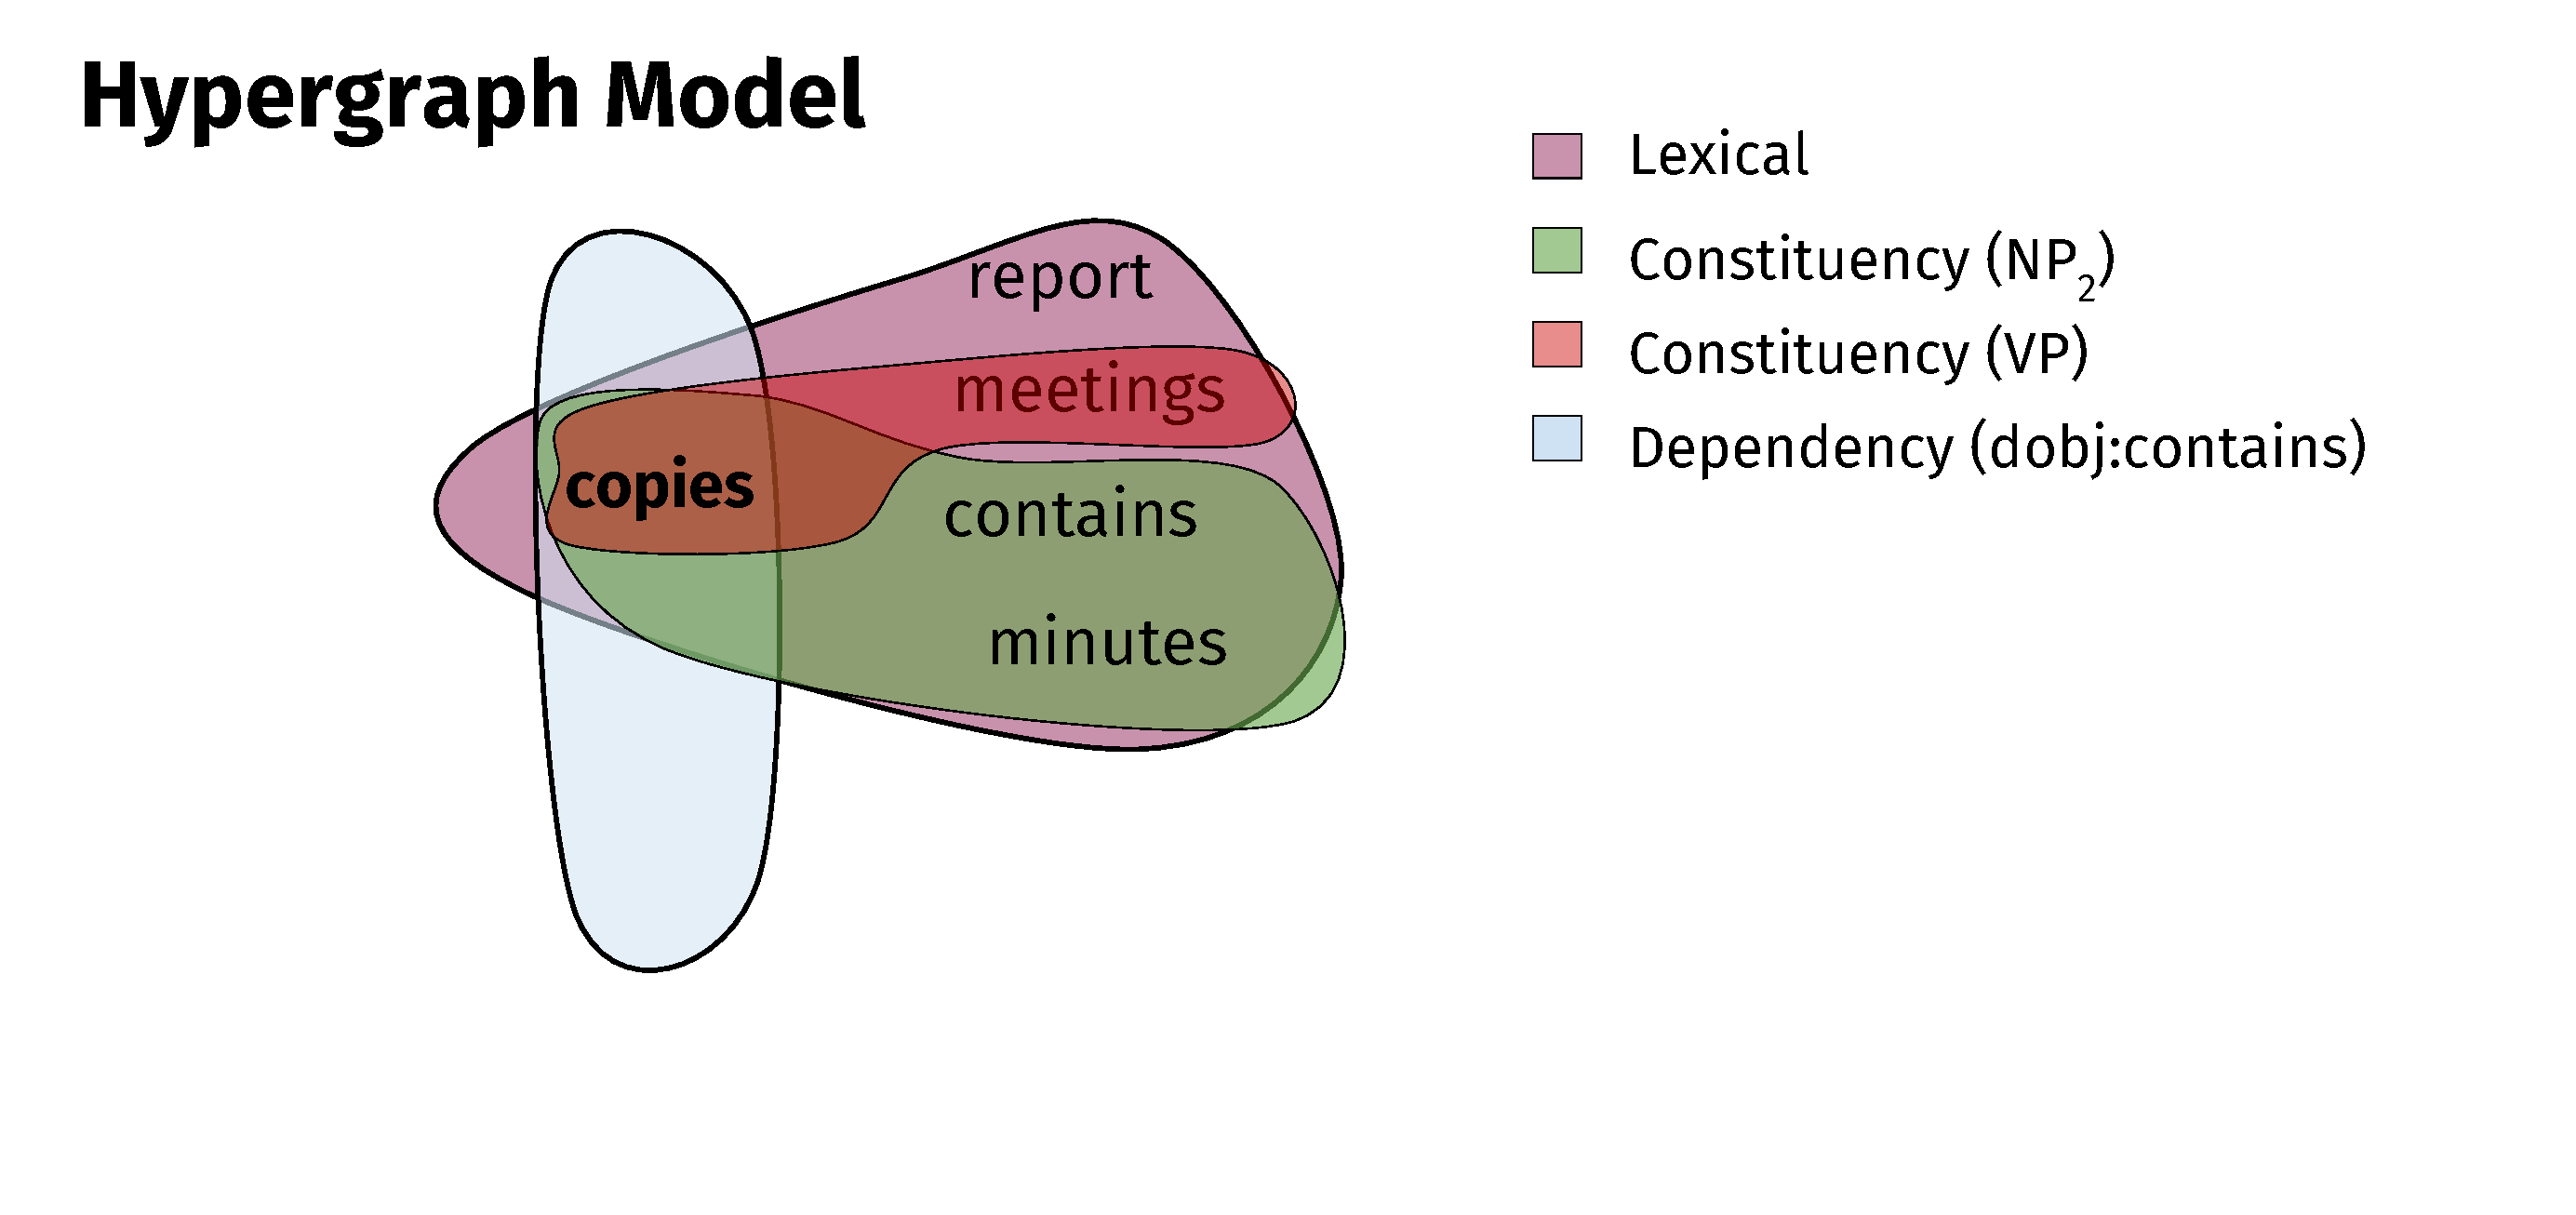
\includegraphics[width=1\linewidth]{image2/Chapitre2/hyper_network_ex_4.pdf}%dep
	\onslide<6>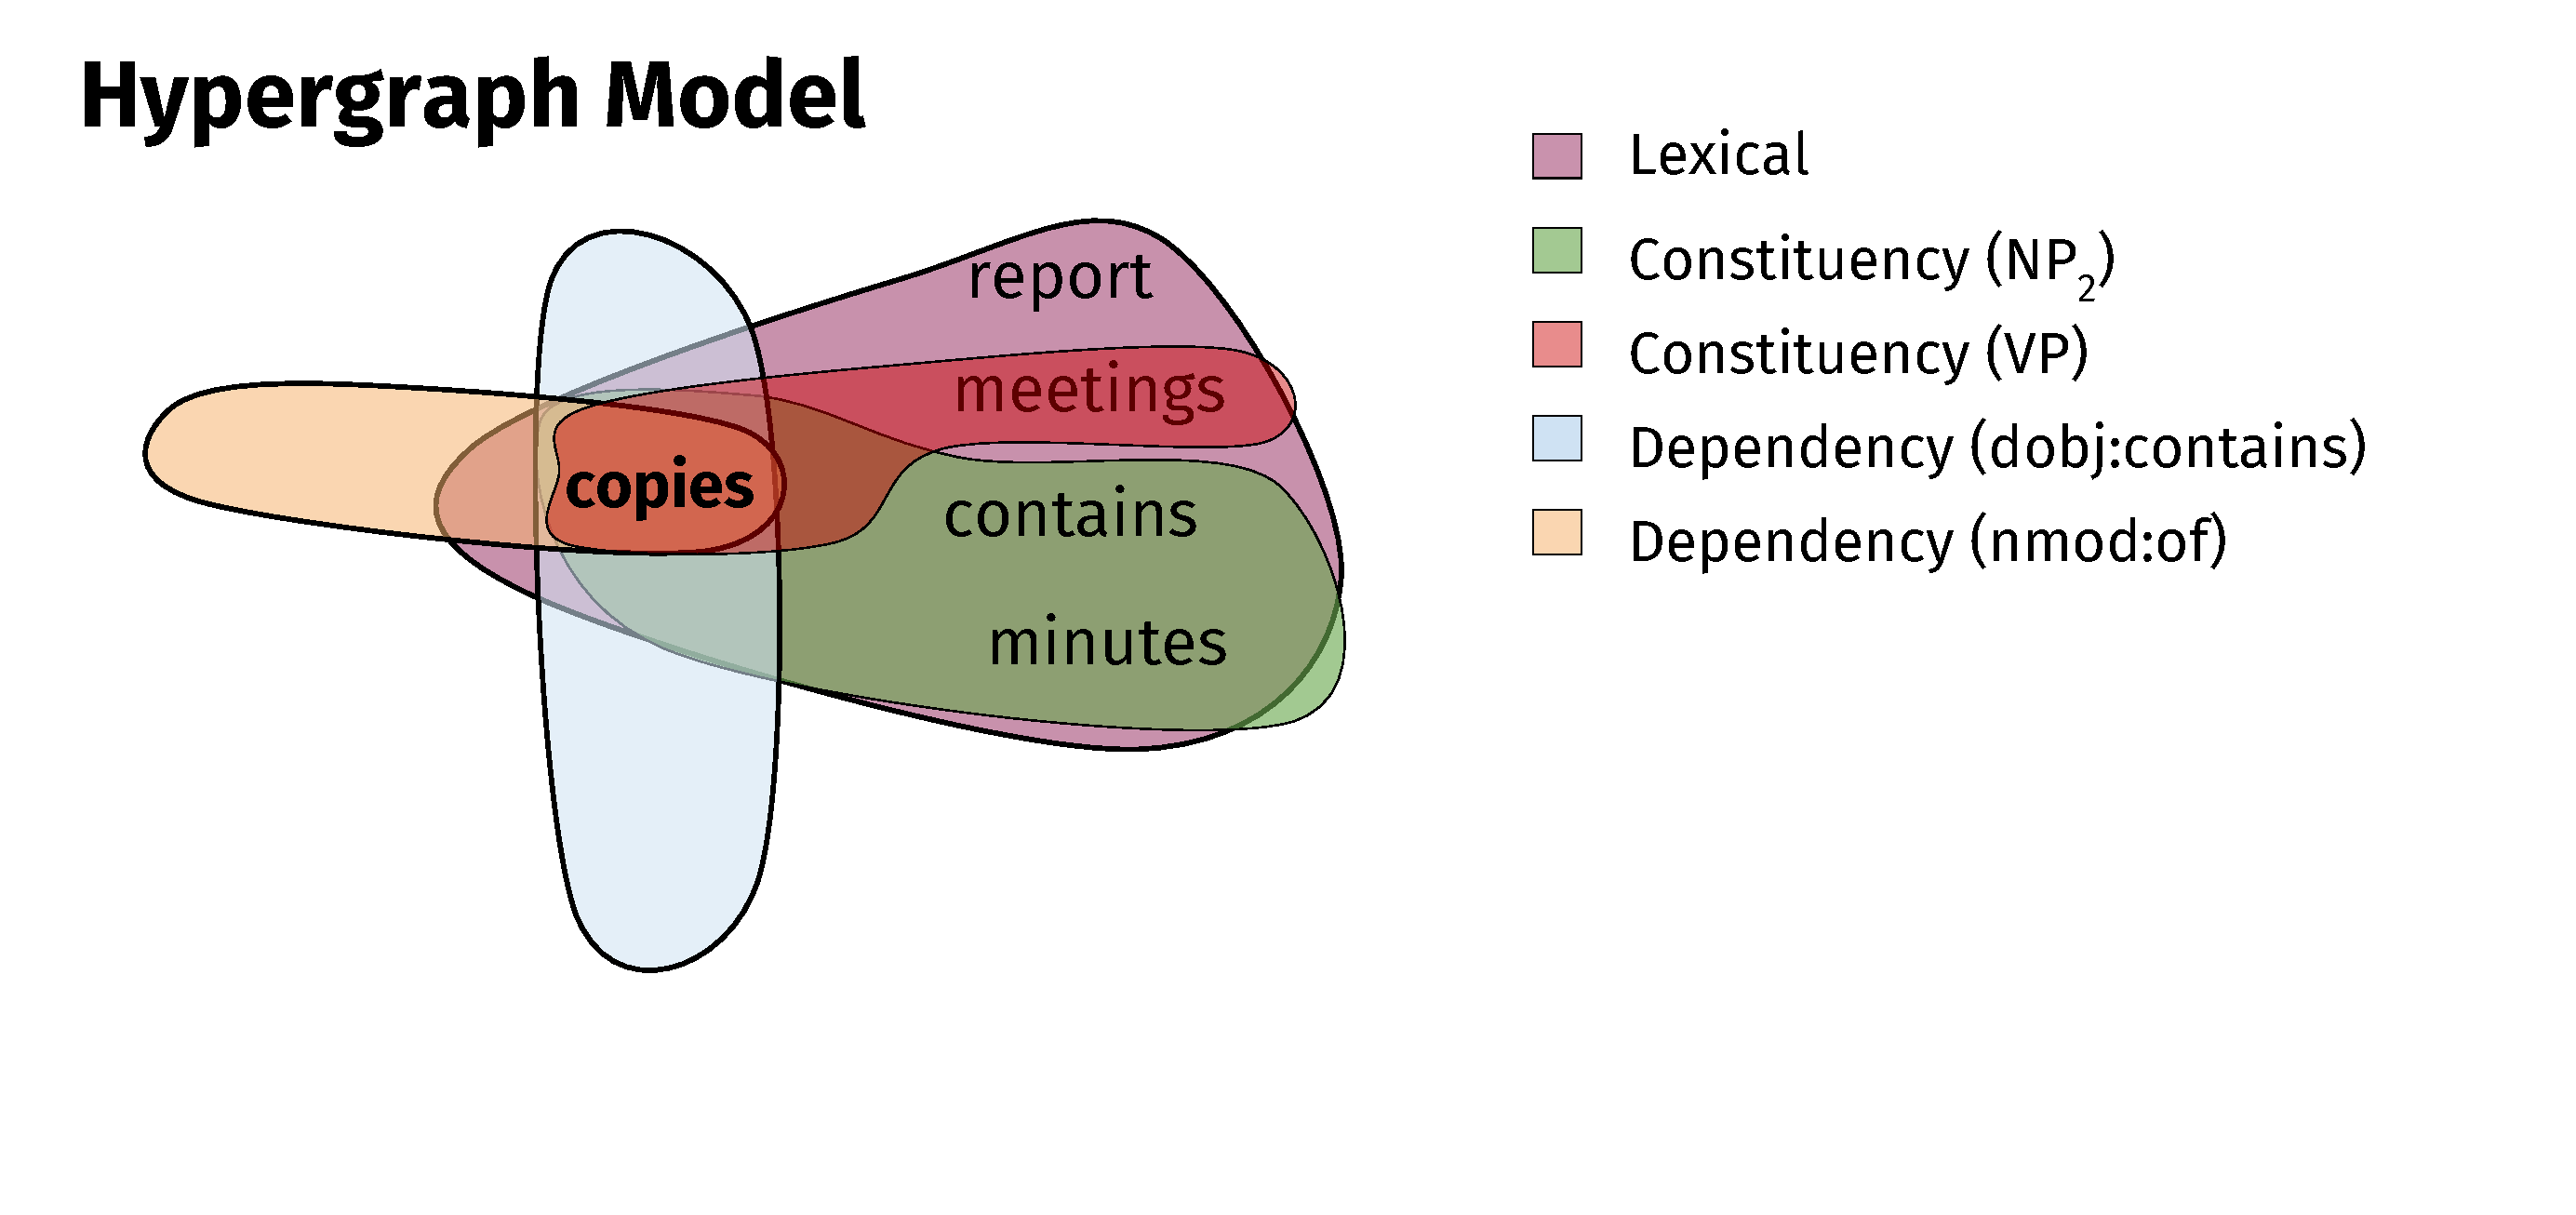
\includegraphics[width=1\linewidth]{image2/Chapitre2/hyper_network_ex_5.pdf}%dep
	\end{overprint}
	\vspace{7cm}
\end{frame}

%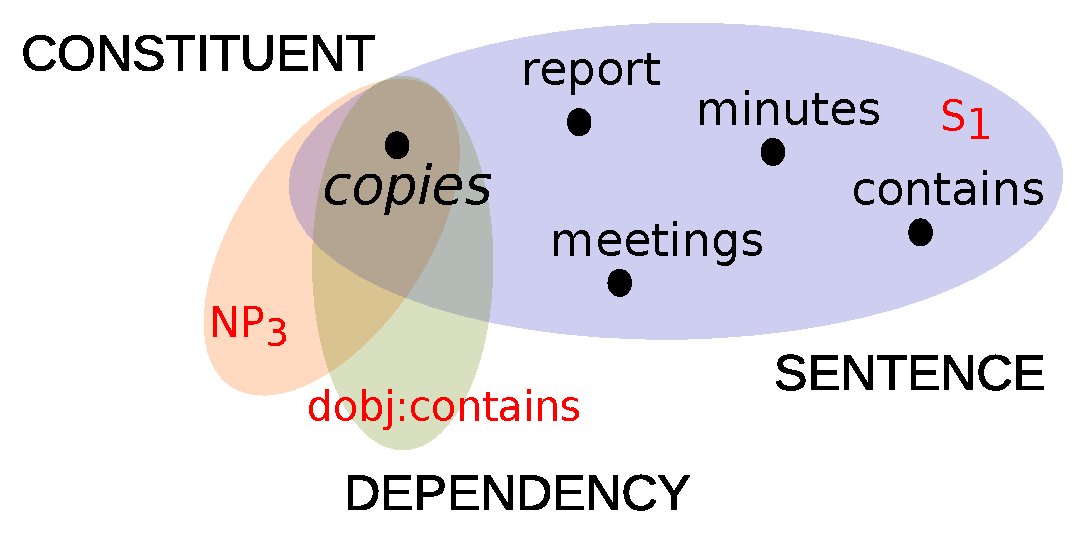
\includegraphics[width=.6\linewidth]{img/hypergraph_copies.pdf} <===== THIS!

\setbeamertemplate{section page}[mytheme]
\section[Contributions in Detail]{Combining Features and Dealing with Sparsity}                  

      
\begin{frame}{Multimedia Fusion Techniques}
\vfill
%\vspace{.5cm}
\begin{itemize}
\item<1-> \large \textbf{Definition}
	\begin{itemize}
	\item<1-> Used in multimedia analysis tasks to integrate multiple media 
	\item<1-> We adapt them to combine textual information

	\item<1-> The goal is to obtain rich insights about the data being treated
	\item<1-> By creating a single representation from heterogeneous information
	\end{itemize}									
\vfill	
\item<2-> \large\textbf{Main fusion operators:}
	\begin{itemize}
	\item<2-> Early Fusion $E_\alpha(\cdot)$, 
	\item<2-> Late Fusion $L_\beta(\cdot)$, 
	\item<2-> Cross Fusion $X_\gamma(\cdot)$
%	\item $\alpha$ and $\beta$: Assign an importance weight to each of their operators 
%	\item $\gamma$: number of top similar items to take from the similarity space
	\end{itemize}

\end{itemize}
\hfill
\end{frame}




\begin{frame}{Early and Late Fusion}
\centering
\onslide<1->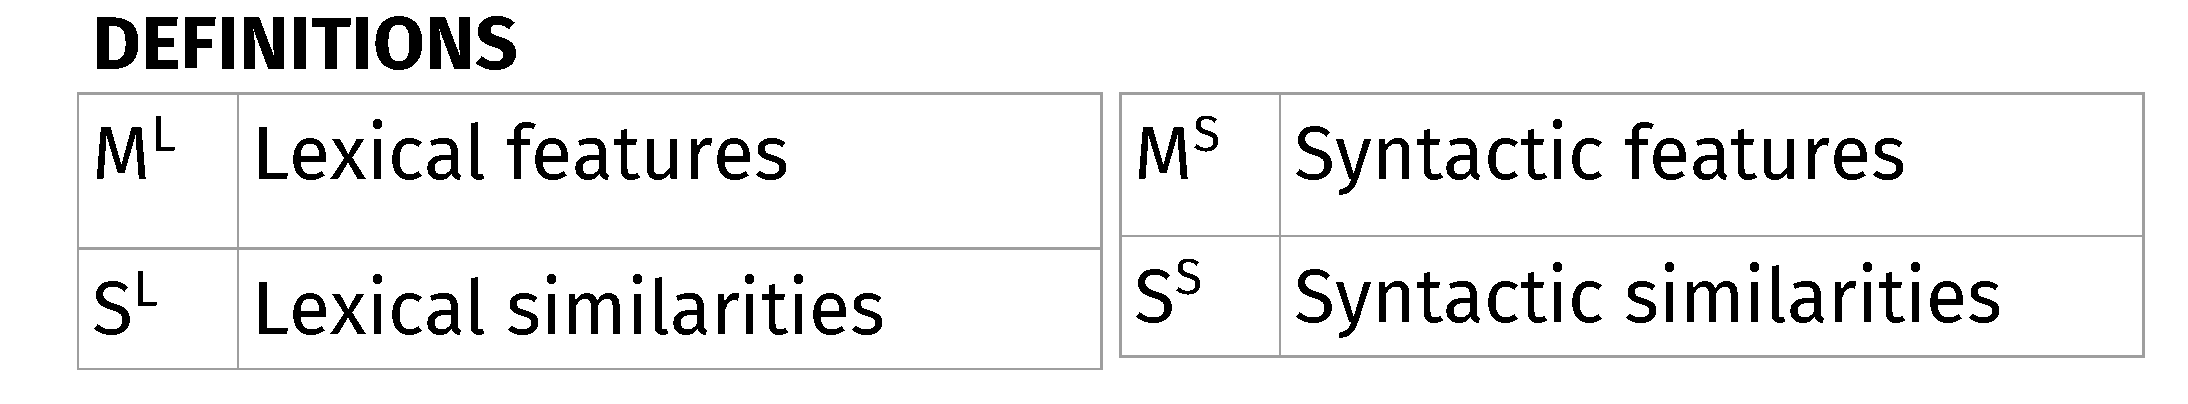
\includegraphics[width=.8\linewidth]{image2/Chapitre3/definition_S_L.pdf}
\vfill
\begin{columns}
	\column{0.5\textwidth}
	\begin{minipage}[c][0.5\textheight][c]{\linewidth}
		\centering
		\onslide<1->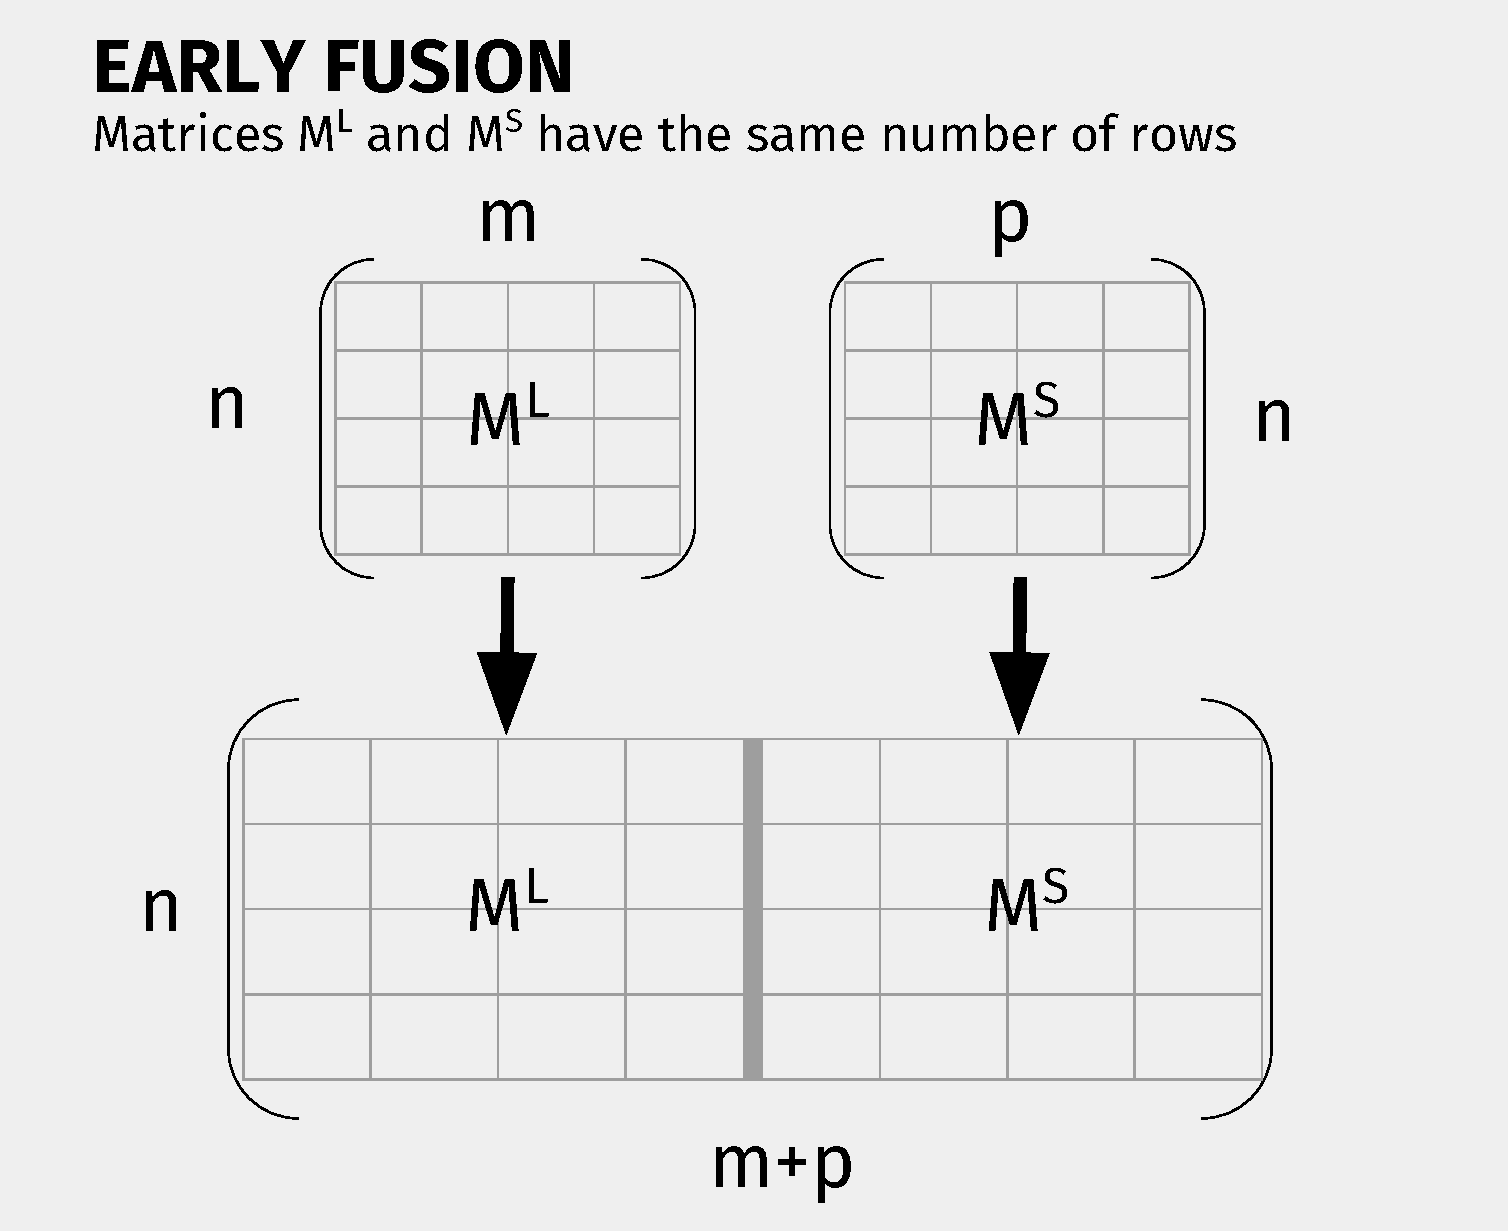
\includegraphics[width=1\linewidth]{image2/Chapitre3/ef_diag}
		\end{minipage}
		\column{0.5\textwidth}
	\begin{minipage}[c][0.5\textheight][c]{\linewidth}
		\centering
		\onslide<2->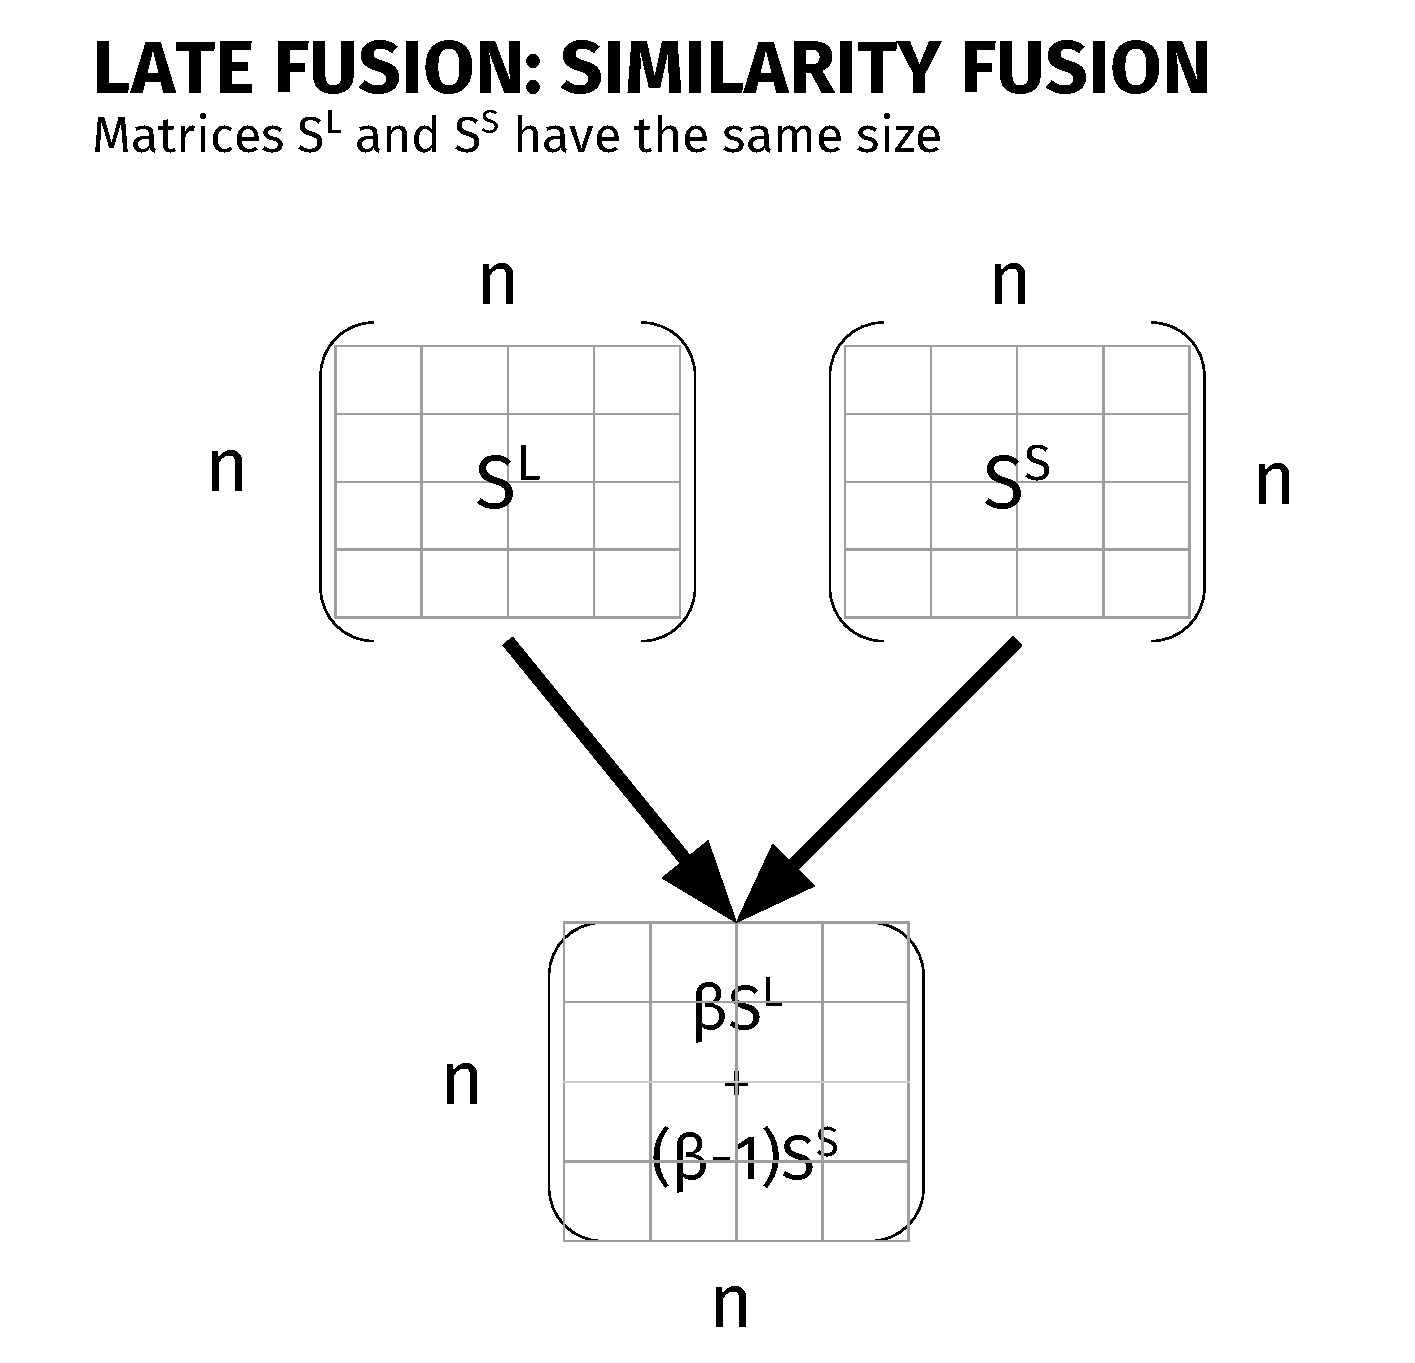
\includegraphics[width=1\linewidth]{image2/Chapitre3/lf2_diag.pdf}
	\end{minipage}
\end{columns}




\end{frame}



\begin{frame}{Cross Fusion}
\begin{center}
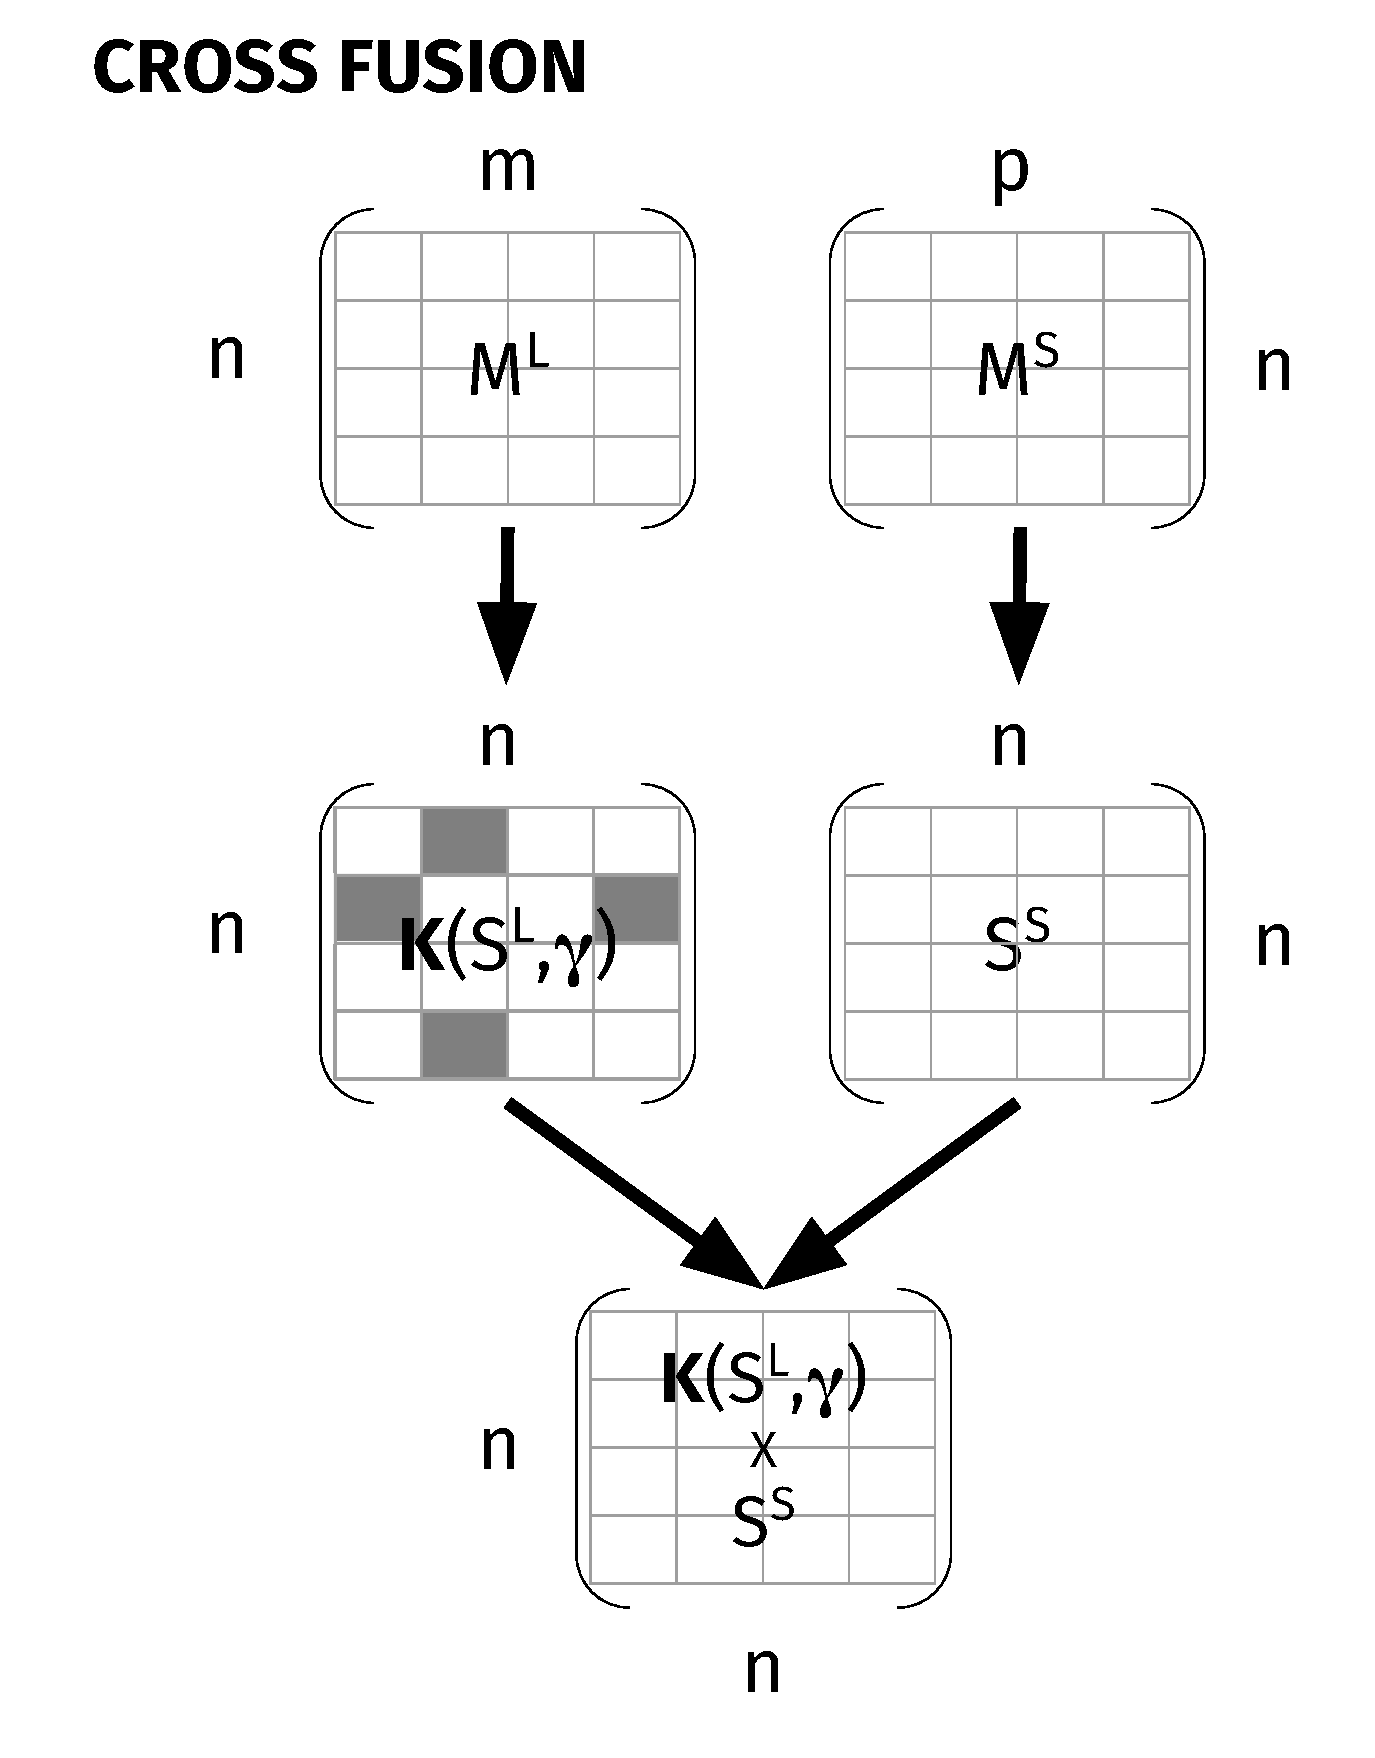
\includegraphics[width=.55\linewidth]{image2/Chapitre3/xf_diag.pdf}
\end{center}
\end{frame}


\begin{frame}{Hybrid Fusion}
\begin{itemize}
%\item \large Combining fusion operators
%	\begin{itemize}
%	\item Chaining together fusion functions to leverage the complementarity of the different features
%	\end{itemize}
\item<1-> \textbf{Combining fusion operators}

\begin{itemize}
\item<1-> Applying one function to the result of another to produce a new fusion function
\end{itemize}
\begin{overprint}
	\onslide<2>
		\begin{itemize}
		\item \textbf{First Degree} 
			\begin{itemize}
			\item $E(\mlex,\msyn)$, $L(\ssyn,\mlex)$ 
			\item \textbf{Cross Feature Fusion}: $X_F(S^S, M^L)$
			\item \textbf{Cross Similarity Fusion}: $X_S(S^S, S^L)$
			\end{itemize}
		\end{itemize}
		\centering
		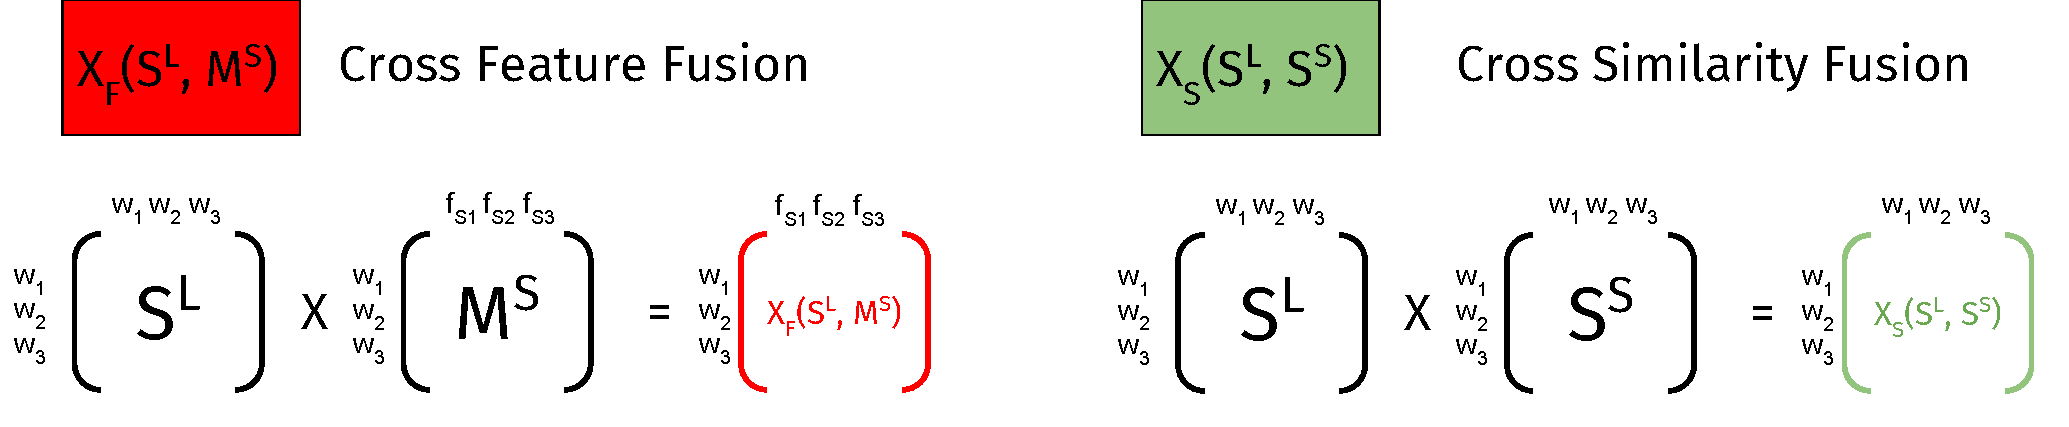
\includegraphics[width=1\linewidth]{image2/Chapitre2/xFFusion.pdf}
	\onslide<3>
		\begin{itemize}
		\item \textbf{Second Degree} 
			\begin{itemize}
			\item \textbf{Cross Feature Early Fusion}: $X_F(S^T , E(M^S, M^L ))$
			\item \textbf{Late Cross Feature Fusion}: $L(M^T, X_F (S^T , M^T ))$
			\end{itemize}
		\end{itemize}
		\centering
		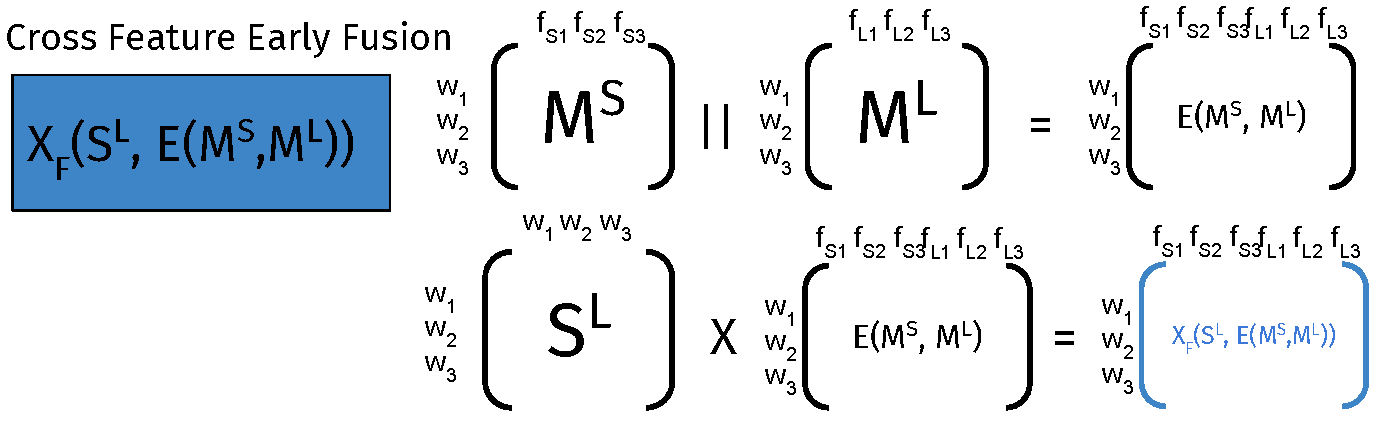
\includegraphics[width=1\linewidth]{image2/Chapitre2/XFEF.pdf}

	\onslide<4>
		\begin{itemize}
		\item \textbf{Higher Degree}
			\begin{itemize}
			\item Triple Early Double Late Cross Feature Fusion: $E(M_L , E(E(M_T , L(M^T , X_F (S^T , M^T ))) , L(M^L , X_F (S^S , M^L))))$
			\end{itemize}
		\end{itemize}
		
\end{overprint}
	

\end{itemize}
\vfill
\end{frame}

\begin{frame}{High Degree Fusion}
\begin{itemize}
\item[] \large \textbf{Higher Degree Operator }
\end{itemize}
\begin{overprint}
	\onslide<1>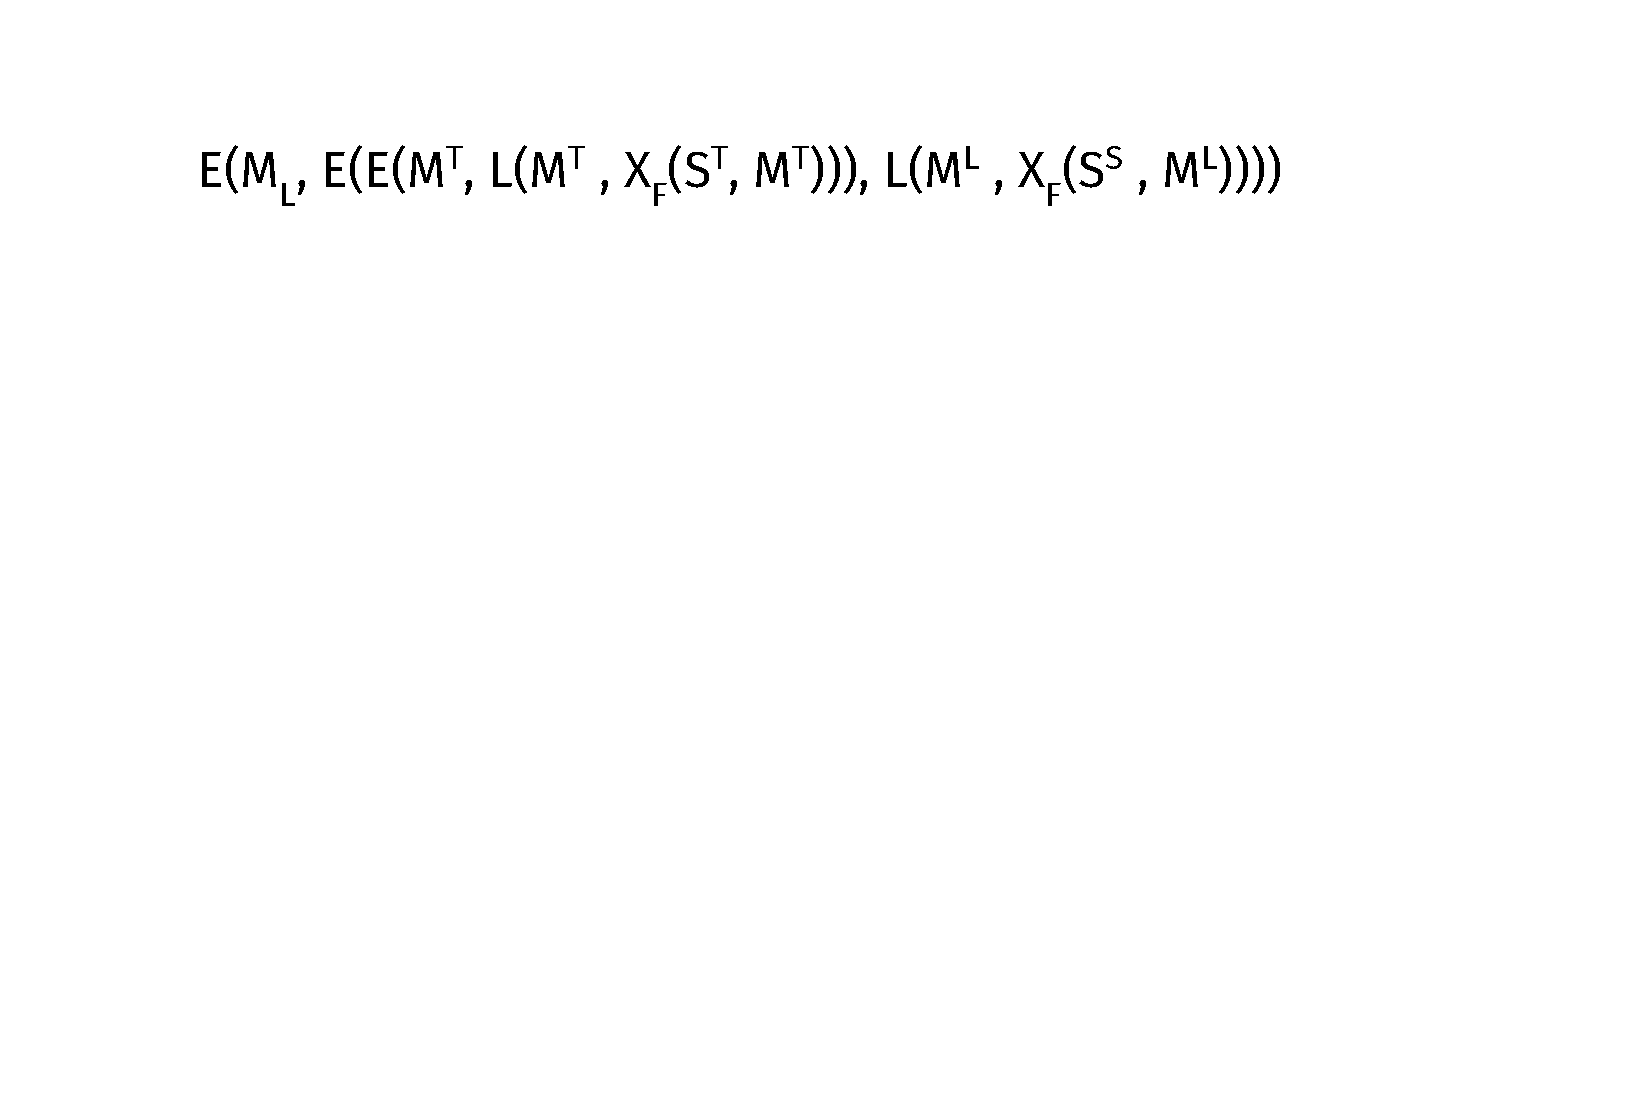
\includegraphics[width=1\linewidth]{image2/Chapitre2/hybrid_fusion0.pdf}%lexical
	\onslide<2>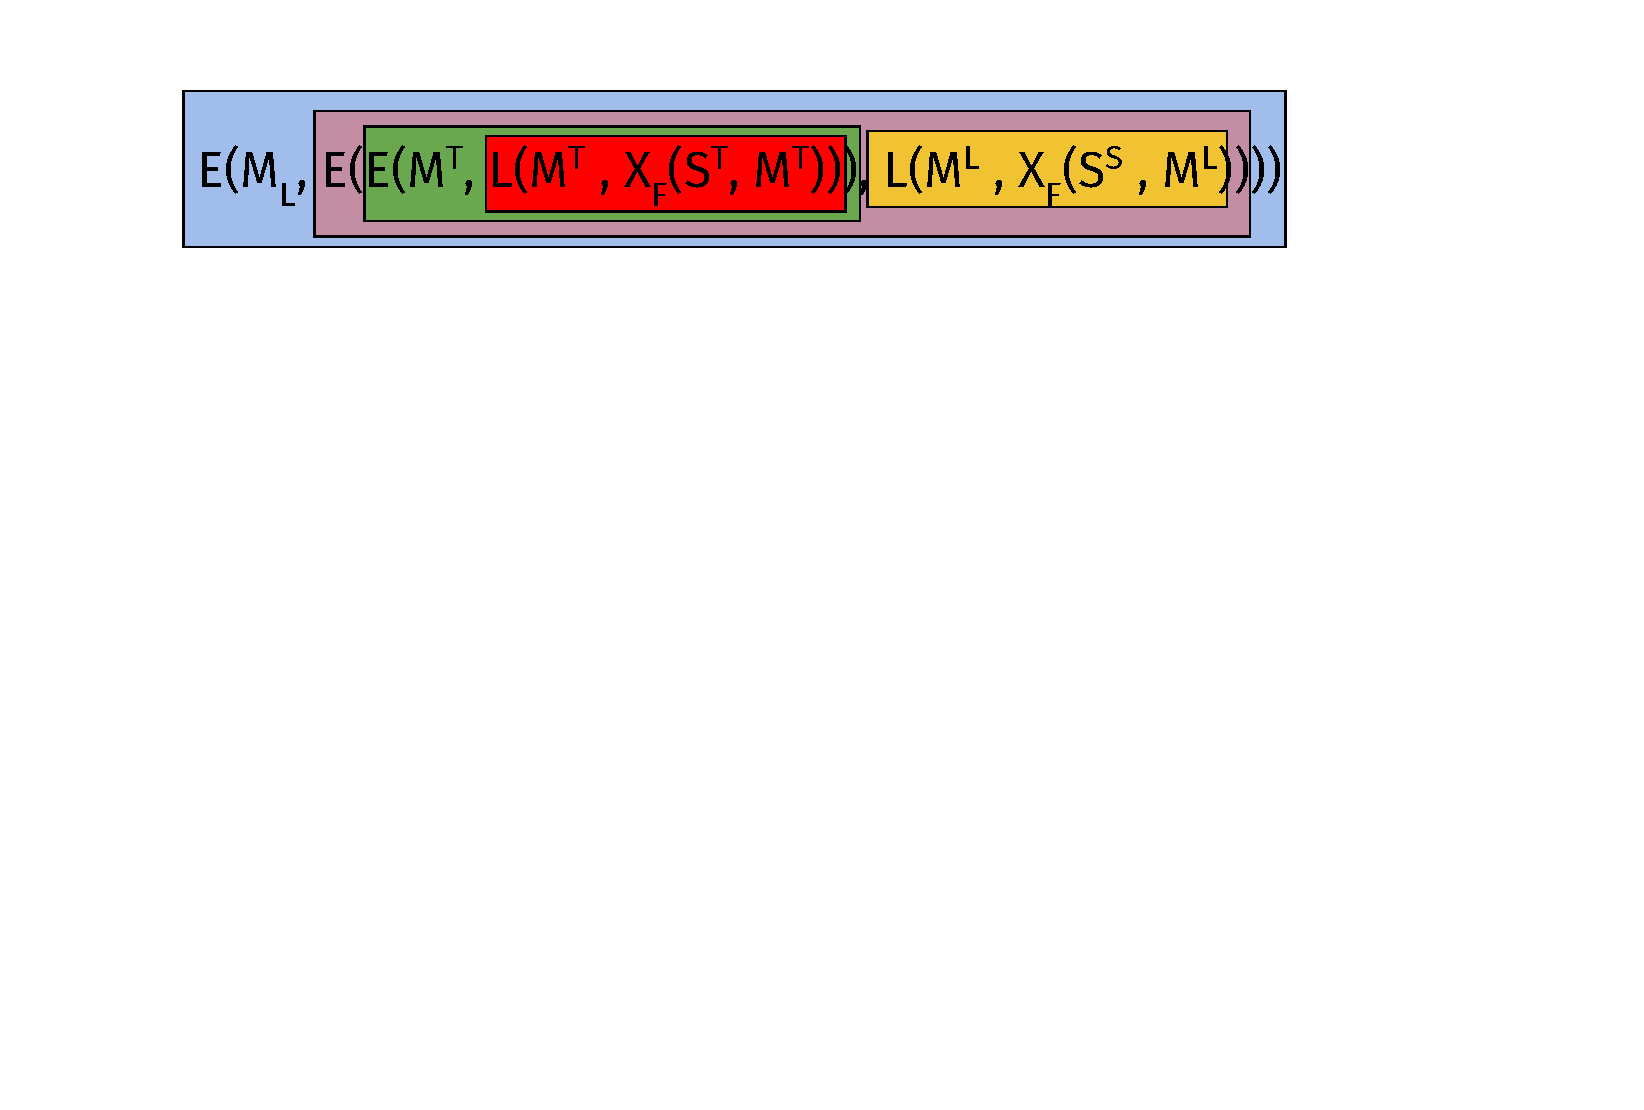
\includegraphics[width=1\linewidth]{image2/Chapitre2/hybrid_fusiona.pdf}%lexical
	\onslide<3>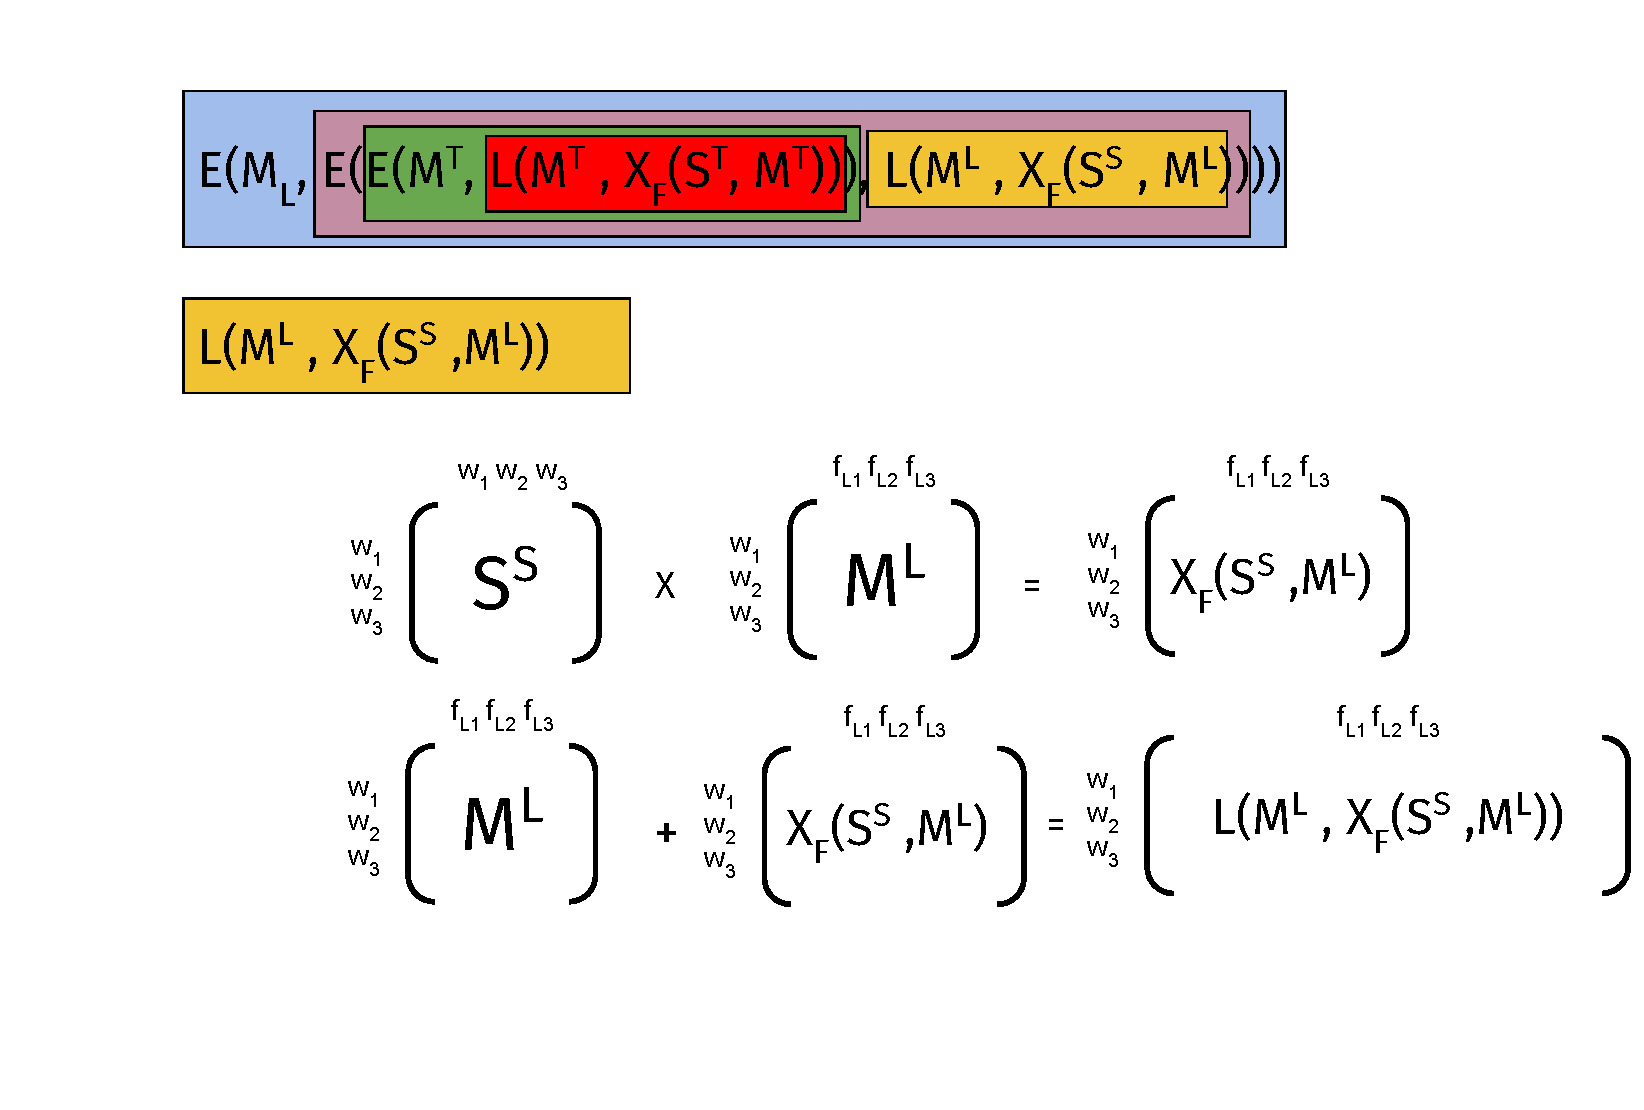
\includegraphics[width=1\linewidth]{image2/Chapitre2/hybrid_fusion1.pdf}%lexical
	\onslide<4>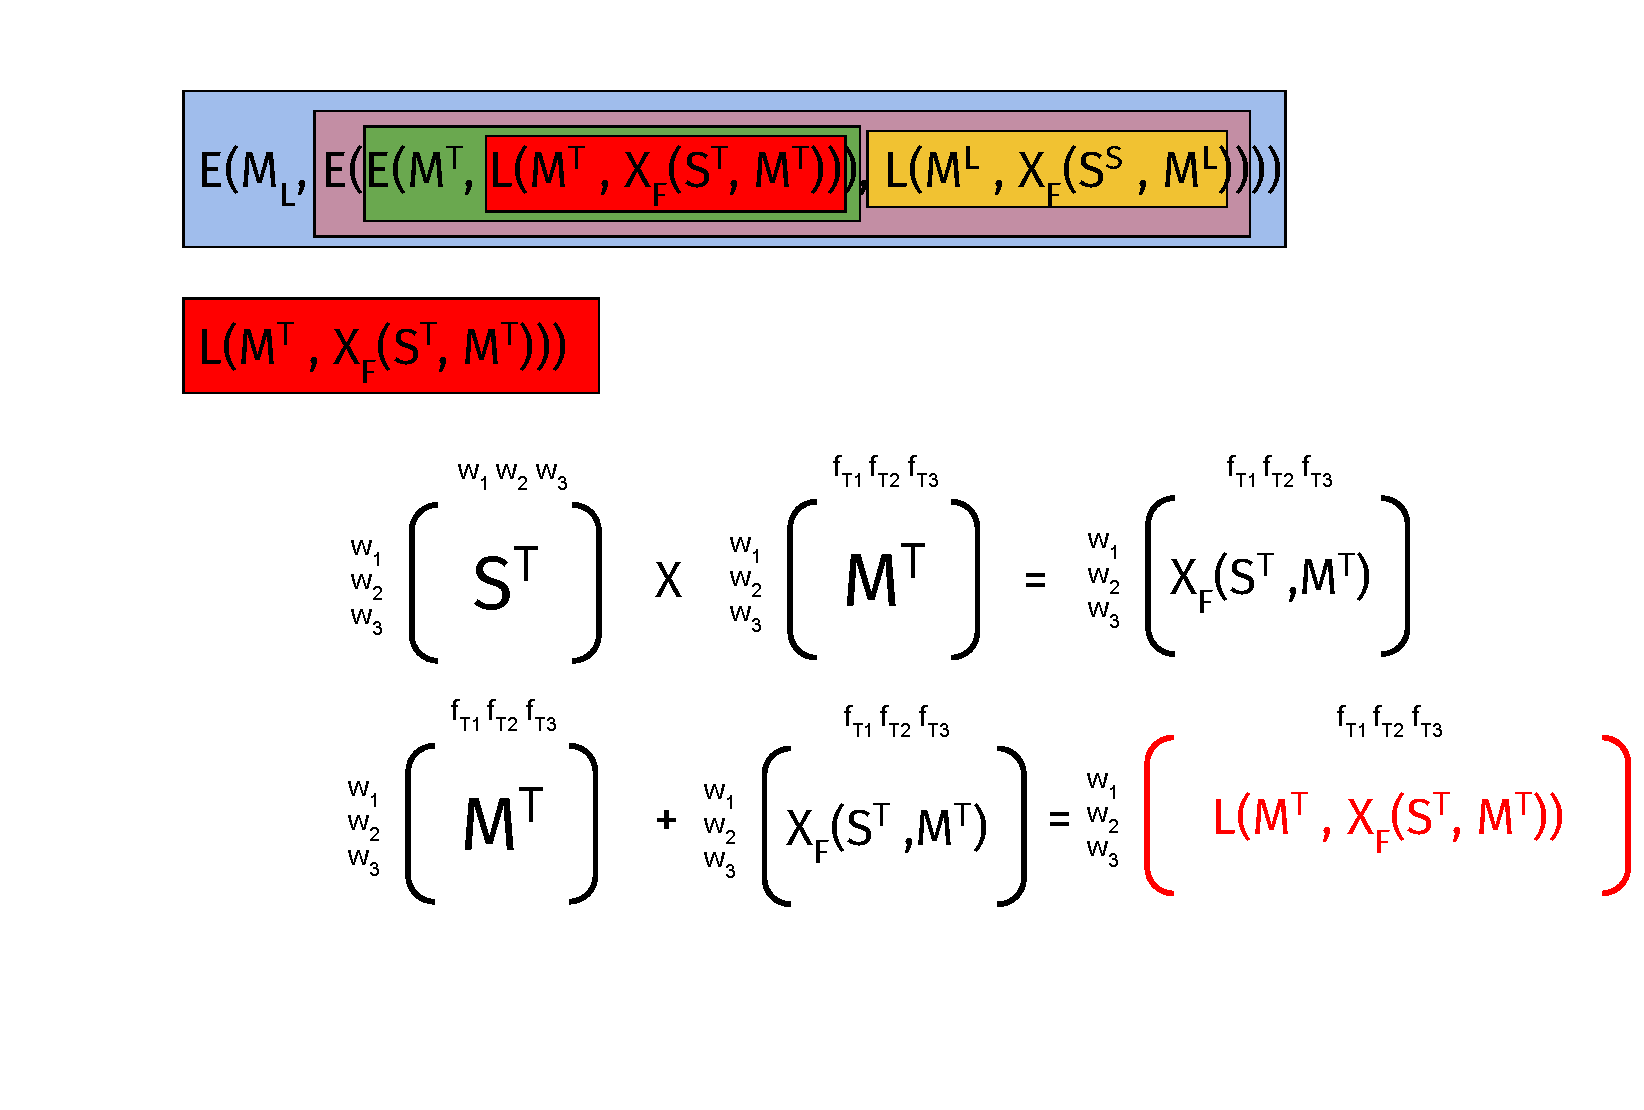
\includegraphics[width=1\linewidth]{image2/Chapitre2/hybrid_fusion2.pdf}%constit
	\onslide<5>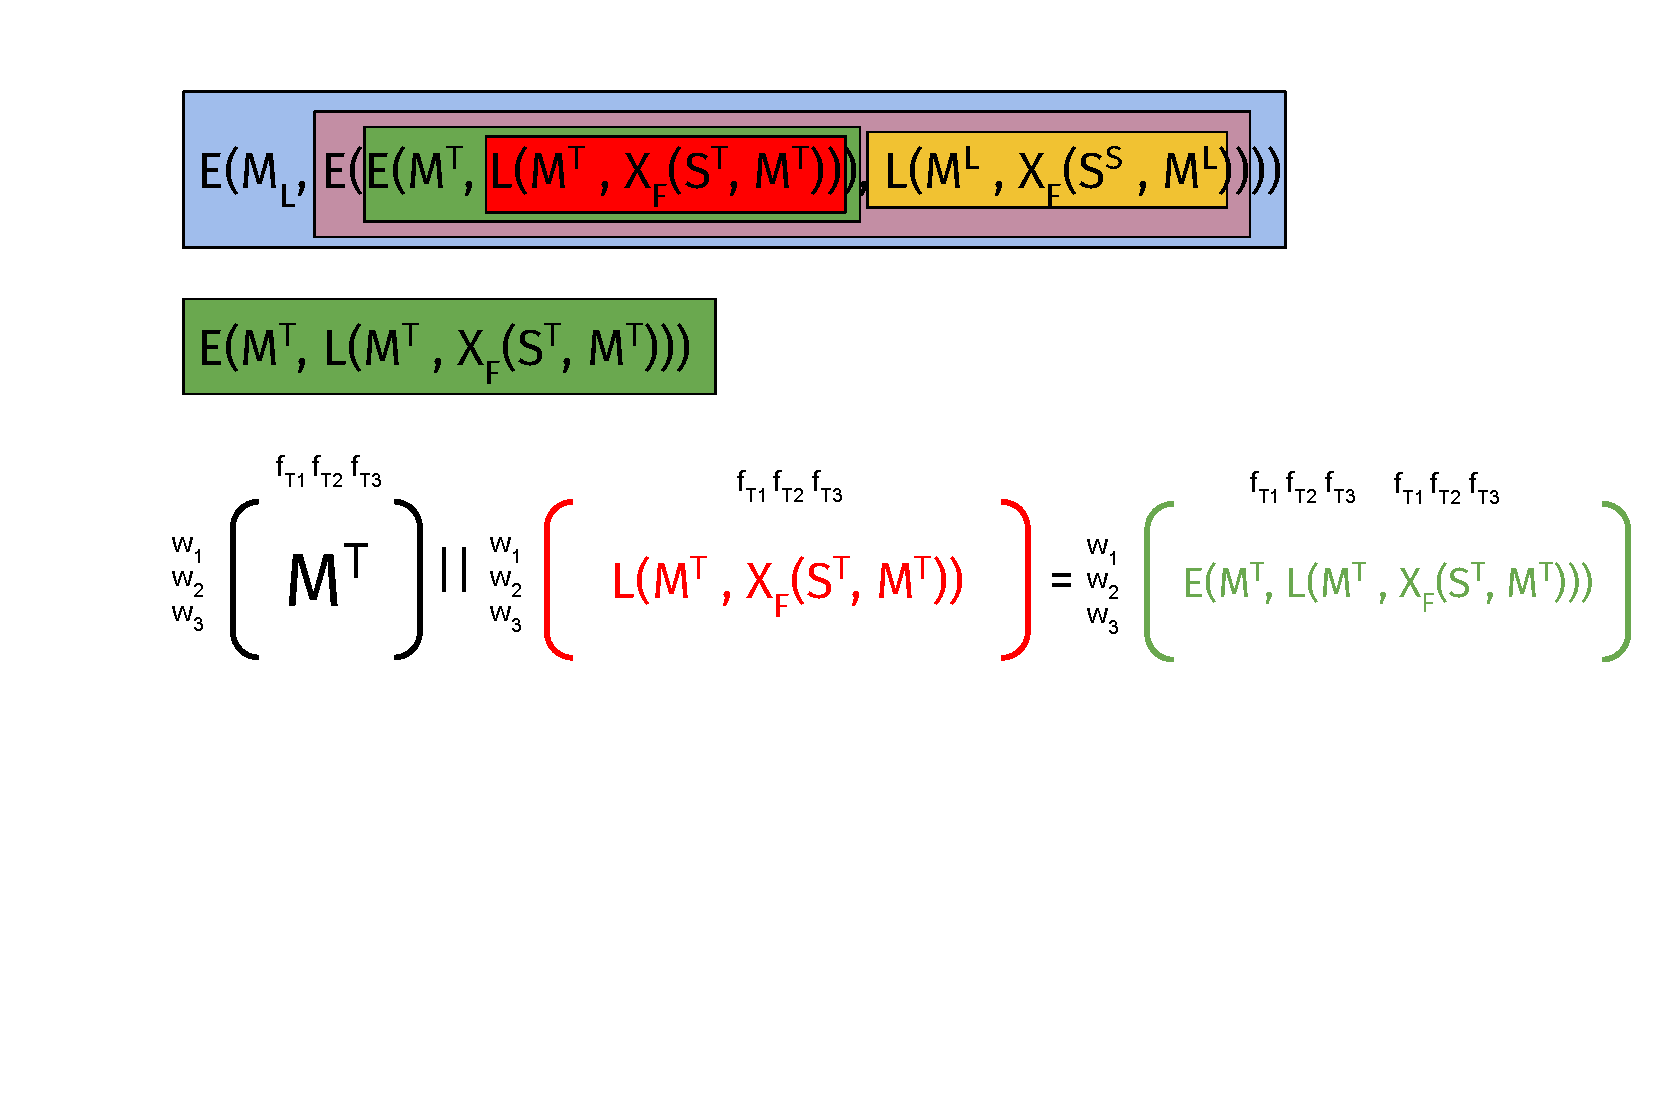
\includegraphics[width=1\linewidth]{image2/Chapitre2/hybrid_fusion3.pdf}%constit
	\onslide<6>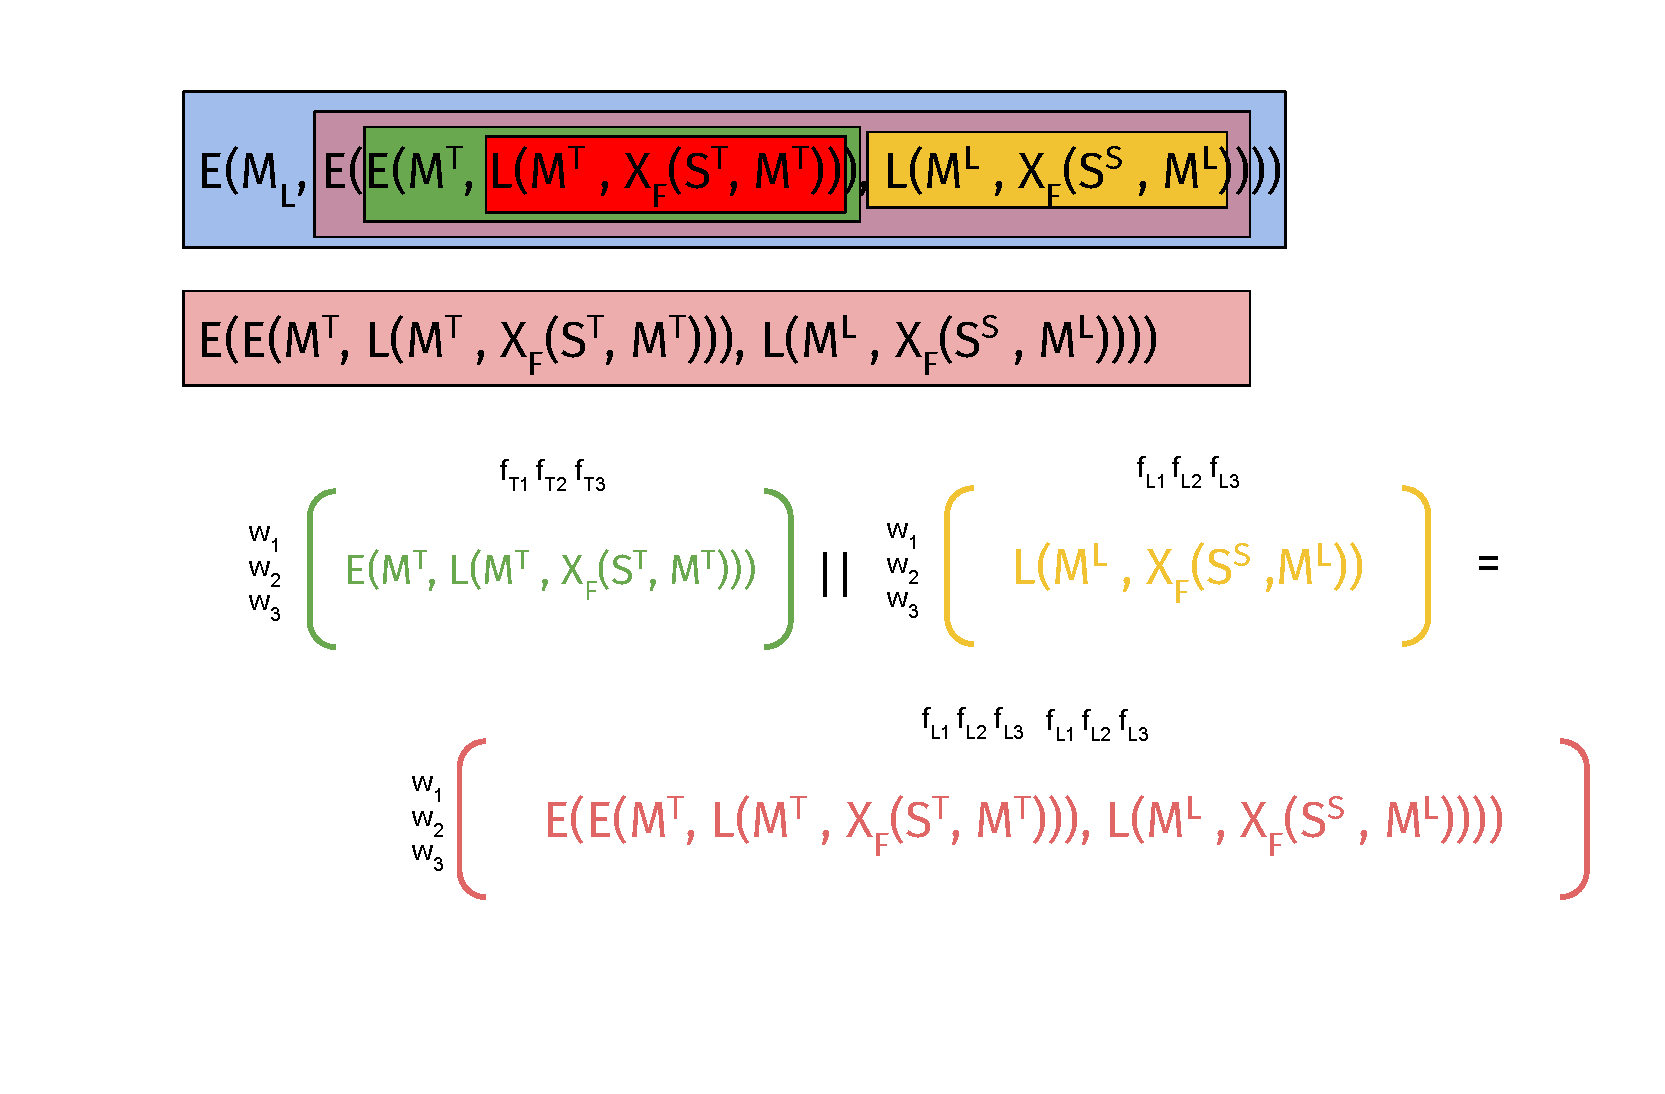
\includegraphics[width=1\linewidth]{image2/Chapitre2/hybrid_fusion4_a.pdf}%dep
	\onslide<7>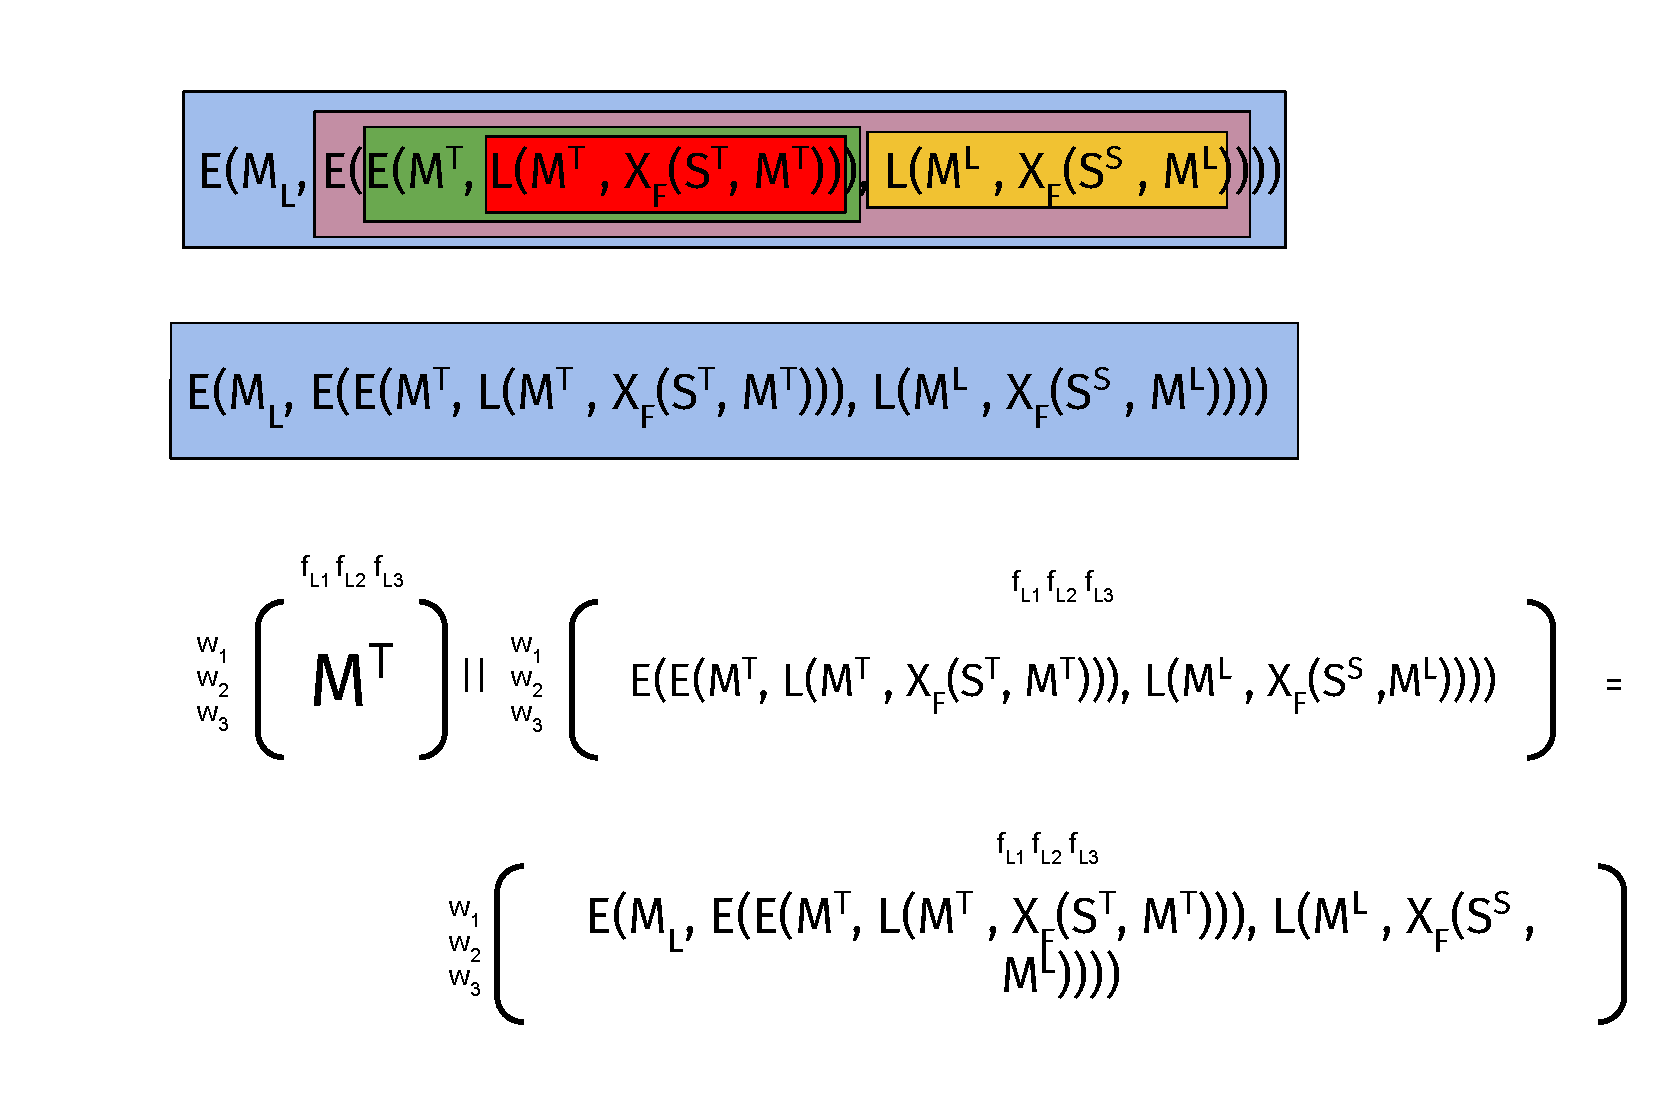
\includegraphics[width=1\linewidth]{image2/Chapitre2/hybrid_fusion4.pdf}%dep
\end{overprint}
\end{frame}






\section[Contributions in Detail]{Finding Communities in the Network}


\begin{frame}{Introduction}

	\begin{itemize}
		\item<1-> \large \textbf{Language networks tend to be scale-free}	
			\begin{itemize}
				\item<1-> There are certain nodes (hubs) that are very well connected forming communities within the network
			\end{itemize}
%
		\item<2-> \large \textbf{Seminal approaches}
			\begin{itemize}
				\item<2-> Hyperlex \cite{2004.Veronis}
				\item<2-> University of York (UoY) \cite{2007.Klapaftis.UOY}
			\end{itemize}
		\item<3-> \textbf{Limitations of existing approaches}
		\begin{itemize}
			\item<3-> Single typed networks
			\item<3-> Large number of parameters
		\end{itemize}
		\item<4-> \textbf{Proposition}
		\begin{itemize}
				\item<4-> Be able to exploit different types of linguistic information (lexical or syntactic co-occurrence)
				\item<4-> Keep  the number of parameters low and allow for their automatic adjusting according to the network's nature
%				\item Use a robust and interpretable similarity measure
		
		\end{itemize}
\end{itemize}
\vspace{\textheight}	
\end{frame}
\begin{frame}{Proposed Method}
  \centering
  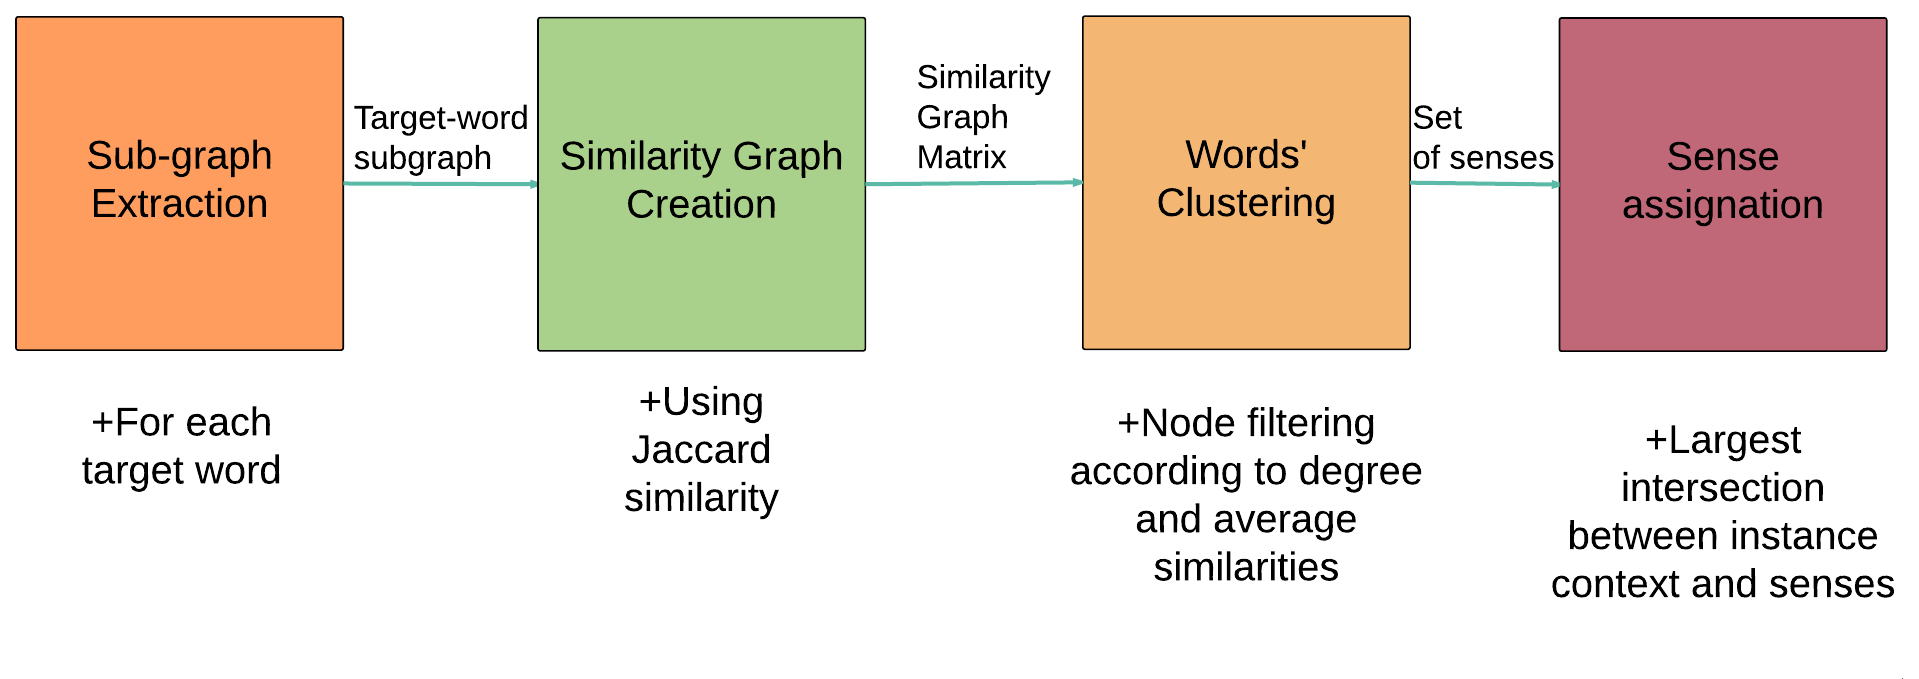
\includegraphics[width=1\linewidth]{img/wsd_wsi.png}

\end{frame}


\begin{frame}<presentation:0>[noframenumbering]{Leveraging the network communities} 
\begin{enumerate}
\item Link some words together with a color overlay to represent possible communities (clusters/groups) of same sense words. 
\item Argue that thanks to the heterogeneous info contained in the structure, we can relate words according to different linguistic properties 

\end{enumerate}
\end{frame}

\section[Applications to NLP]{Hypergraph Model Instantiation}



\begin{frame}<presentation:0>[noframenumbering]{Introduction}
\large \textbf{Applications}
\vspace{.5cm}
\begin{itemize}
\item \large \textbf{We instantiate our proposed linguistic resource}
\begin{itemize}
\item Based on the English Wikipedia corpus
\end{itemize}
\item \large \textbf{Use the proposed model  to solve two NLP tasks}
	\begin{itemize}
	\item Named Entity Recognition 
	\item Word Sense Induction and Disambiguation
	\end{itemize}
\vspace{.3cm}
\item \large \textbf{These experiments have two main objectives}
	\begin{itemize}
	\item Test the effectiveness of fusion enriched representations (heterogeneity + less sparse spaces)
	\item Leverage the structure of the network built following our proposed model
	\end{itemize}

\end{itemize}
\vspace{\textheight}
\end{frame}

\subsection{Introduction}
\begin{frame}{Hypergraph Model Instantiation}
\begin{itemize}
\item<1-> \large \textbf{Apply our proposed linguistic model to a real world corpus}
	\begin{itemize}
	\item<1-> Use the English Wikipedia as input and generate a textual structure following the proposed network model
	\end{itemize}
%\item<2-> \large \textbf{We provide two resources}
%\begin{itemize}
%	\item<2-> A syntactically annotated English Wikipedia corpus (SAEWD)
%	\item<2-> A Wikipedia-based enriched hypergraph linguistic model 
%\end{itemize}
\item<2-> \large \textbf{Steps performed}	
\begin{itemize}
	\item<2->[] \begin{center}
		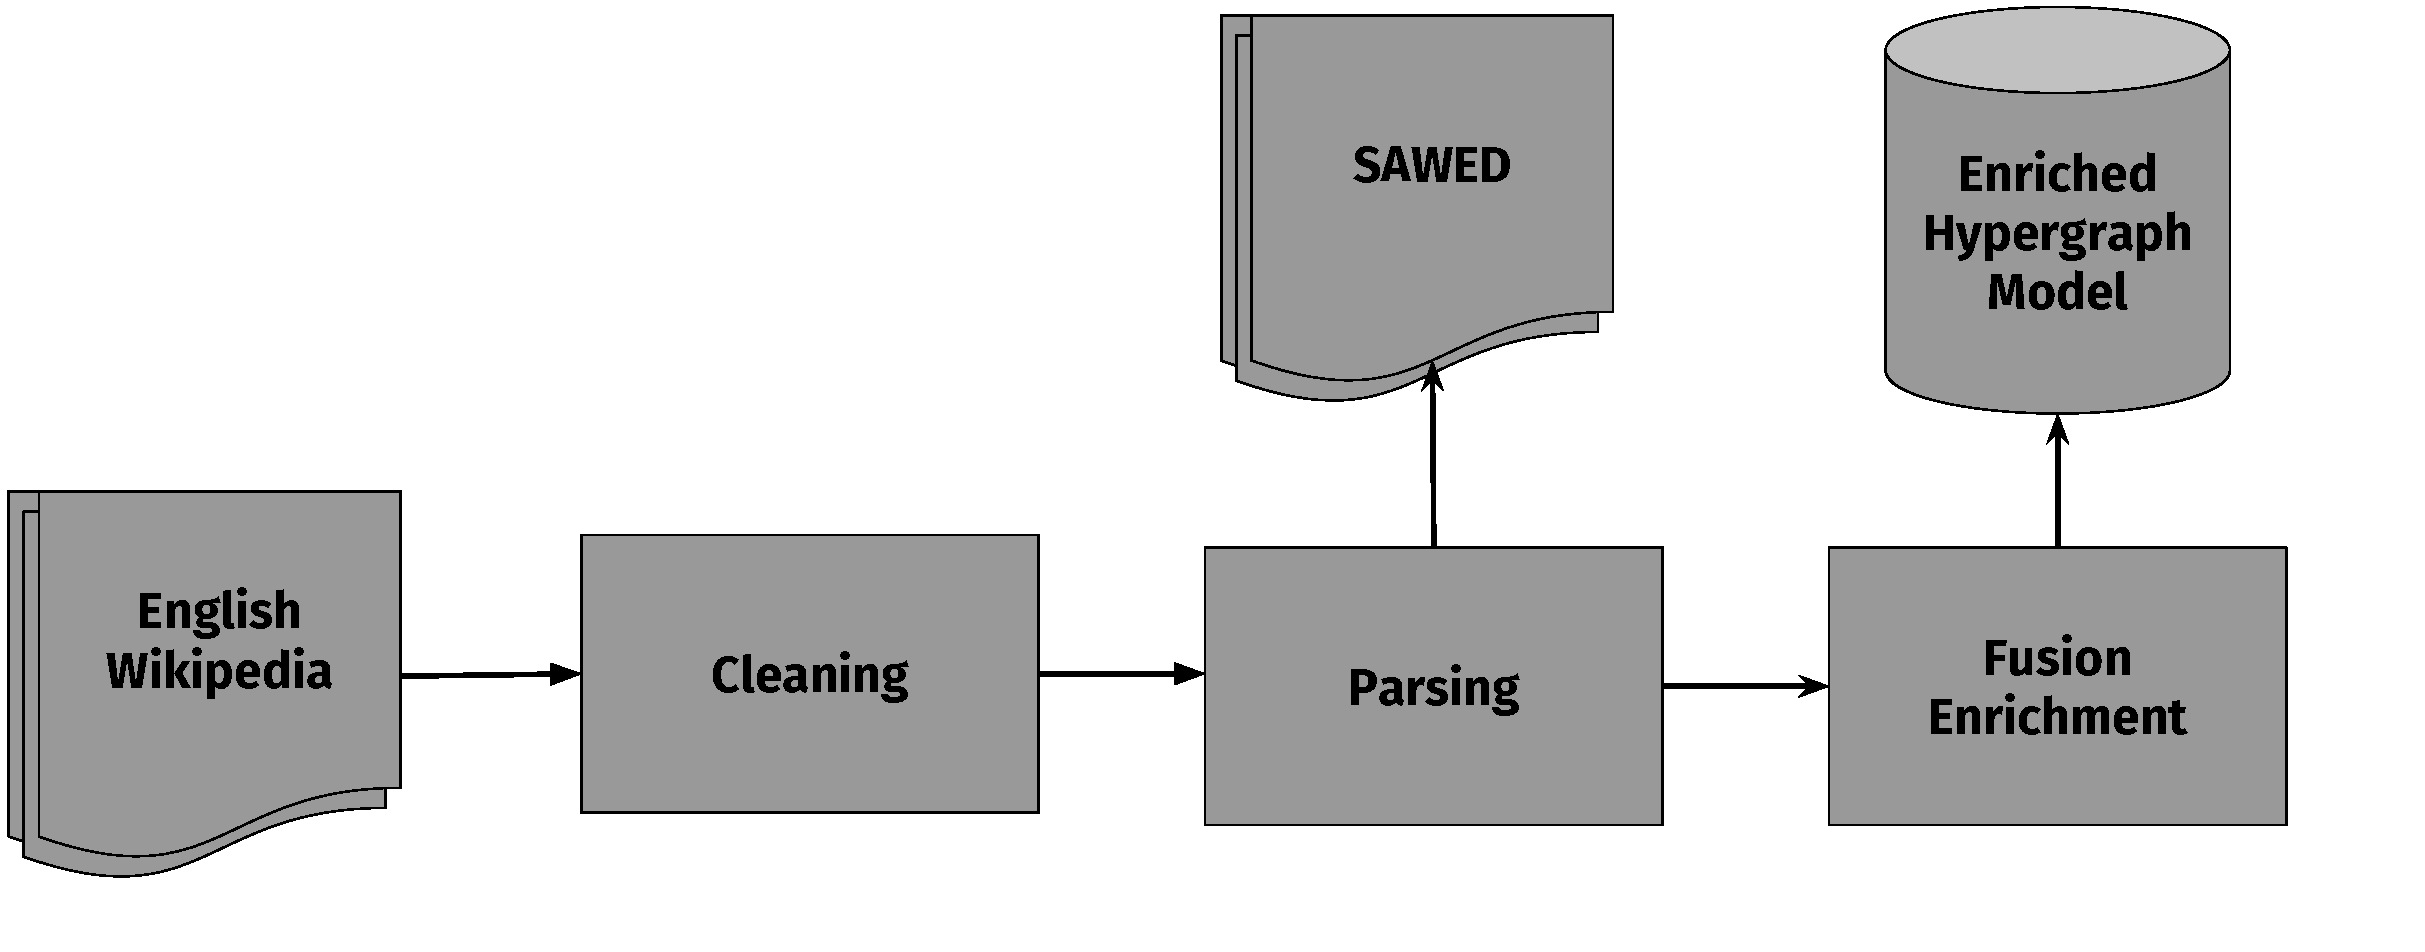
\includegraphics[width=\linewidth]{image2/Chapitre7/saewd}
		\end{center}

\end{itemize}

\end{itemize}

\end{frame} 


\begin{frame}{SAEWD: Parsed sample}


			 	\centering	           
	\adjustbox{max height=\dimexpr\textheight-6.5cm\relax,
	           max width=\textwidth}{
\begin{tabular}{llllll}
 \multicolumn{6}{l}{\textit{FILENAME wiki\_00.parsed}}                                           \\ \hline
  \textbf{token}   & \textbf{lemma}   & \textbf{POS} & \textbf{constituency}                      & \textbf{head} & \textbf{dependency} \\ \hline
 \multicolumn{6}{l}{\textit{\%\%\#PAGE Anarchism}}                                         \\ \hline
  {$\vdots$}      &      {$\vdots$}   &  {$\vdots$}   &     {$\vdots$}                              &    {$\vdots$}  &     {$\vdots$}       \\  \hline
 \multicolumn{6}{l}{\textit{\%\%\#SEN 25  9}}                                             \\ \hline
						 A       & a       & DT  & NP\_22,S\_97                      & 3    & det        \\ %\cline{2-7} 
                         great   & great   & JJ  & NP\_22,S\_97                      & 3    & amod       \\ %\cline{2-7} 
                         brigand & brigand & NN  & NP\_22,S\_97                      & 4    & nsubj      \\ %\cline{2-7} 
                         becomes & become  & VBZ & VP\_44,S\_97                      & 0    & root       \\ %\cline{2-7} 
                         a       & a       & DT  & NP\_18,NP\_20,VP\_44,S\_97        & 6    & det        \\ %\cline{2-7} 
                         ruler   & ruler   & NN  & NP\_18,NP\_20,VP\_44,S\_97        & 4    & xcomp      \\ %\cline{2-7} 
                         of      & of      & IN  & PP\_57,NP\_20,VP\_44,S\_97        & 9    & case       \\ %\cline{2-7} 
                         a       & a       & DT  & NP\_18,PP\_57,NP\_20,VP\_44,S\_97 & 9    & det        \\ %\cline{2-7} 
                         Nation  & nation  & NN  & NP\_18,PP\_57,NP\_20,VP\_44,S\_97 & 6    & nmod       \\ %	\cline{2-7} 
\hline 
\end{tabular}}

\end{frame}


\begin{frame}{Hypergraph Incidence Matrix}
\begin{center}
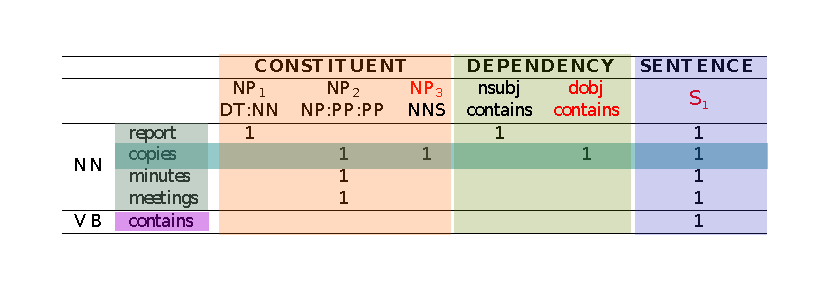
\includegraphics[width=1\linewidth]{img/incidence_aug.pdf}
\end{center}

\end{frame} 



\begin{frame}{Wikipedia Feature Enriched Space}
%\textbf{Target word \textit{priest} and its top 5 most similar words using different representation matrices.}
\begin{itemize}
	\item \textbf{Characteristics of the enriched space}
	\begin{itemize}
	\item Sparsity is reduced
	\item Semantic relatedness differs according to the representation space
	\end{itemize}
\end{itemize}
\begin{tabular}{@{}llllll@{}}
\toprule
                           & \textbf{\begin{tabular}[c]{@{}l@{}}Lexical\\ Features\\ \textcolor{orangeEric}{(5.49\%)}\\$\mlex$\end{tabular}}              
                           & \textbf{\begin{tabular}[c]{@{}l@{}}Syntactic\\ Features\\(4.97\%)\\$\msyn$\end{tabular}}        
                           & \textbf{\begin{tabular}[c]{@{}l@{}}Early\\ Fusion\\(5.23\%)\\$E(\mlex, \msyn)$\end{tabular}}                
                           & \textbf{\begin{tabular}[c]{@{}l@{}}$X_F$\\Fusion\\\textcolor{red}{(16.75\%)}\\$X_F(\ssyn, \mlex)$\end{tabular}}   &
                           \textbf{\begin{tabular}[c]{@{}l@{}}$X_F$\\Fusion\\ (13.45\%) \\$X_F(\slex, \msyn)$\end{tabular}}                 \\ \midrule
\multicolumn{1}{c}{\textbf{priest}} & \begin{tabular}[c]{@{}l@{}}priests\\ nun\\ canton\\ sailor\\ burial\end{tabular} & \begin{tabular}[c]{@{}l@{}}monk\\ regent\\ aedile\\ seer\\ meek\end{tabular} & \begin{tabular}[c]{@{}l@{}}sailor\\ regent\\ nuclei\\ nun\\ relic\end{tabular} & \begin{tabular}[c]{@{}l@{}}vassal\\ regent\\ nun\\ sailor\\ monk\end{tabular} & \begin{tabular}[c]{@{}l@{}}sailor\\ fluent\\ dean\\ nuclei\\ chorus\end{tabular} \\

 \bottomrule

\end{tabular}
\end{frame}

%\begin{frame}{Wikipedia Similarity Enriched Spaces}
%\smaller
%\begin{tabular}{@{}lllllll@{}}
%\toprule
%                           & \textbf{\begin{tabular}[c]{@{}l@{}}Lexical\\ Similarity\\(75.25\%)\\$S^L$\end{tabular}}              & \textbf{\begin{tabular}[c]{@{}l@{}}Syntactic\\ Similarity\\(60.64\%)\\$S^S$\end{tabular}}        & \textbf{\begin{tabular}[c]{@{}l@{}}Early\\ Fusion\\(67.94\%)\\$E(S^L, S^S)$\end{tabular}}                & \textbf{\begin{tabular}[c]{@{}l@{}}Late\\ Fusion\\(83.17\%)\\$L(S^L, S^S)$\end{tabular}}                 & \textbf{\begin{tabular}[c]{@{}l@{}}$X_S$\\ Fusion\\(87.22\%)\\$X_S(\ssyn, \slex)$\end{tabular}}  &
%                           \textbf{\begin{tabular}[c]{@{}l@{}}$X_S$\\
%                           Fusion\\(79.69\%)\\$X_S(\slex,\ssyn)$\end{tabular}}                 
%                           \\ \midrule
%\multicolumn{1}{c}{\textbf{priest}} 
%& \begin{tabular}[c]{@{}l@{}}wholly\\burial\\monk\\lingua\\nuclei\end{tabular} &
%\begin{tabular}[c]{@{}l@{}}regent\\ coach\\ broker\\ dream\\tailor\end{tabular} & \begin{tabular}[c]{@{}l@{}}regent\\slang\\ broker\\rebel\\tiger\end{tabular} & \begin{tabular}[c]{@{}l@{}}regent\\slang\\ seer\\ tutor\\cradle\end{tabular} & \begin{tabular}[c]{@{}l@{}}regent\\vassal\\vizier\\leader\\result\end{tabular} & \begin{tabular}[c]{@{}l@{}}sailor\\nuclei\\nun\\canton\\burial\end{tabular} \\
%
% \bottomrule
%
%\end{tabular}
%\end{frame}

\section[Applications to NLP]{Solving Named Entity Recognition}



\begin{frame}{Introduction}
\begin{itemize}
\item<1-> \large \textbf{NER Objective}
\begin{itemize}
\item<1->  The goal is to automatically discover  mentions that belong to a well-defined semantic category. 

\end{itemize}
\item<2-> \large \textbf{Classic entities types}
	\begin{itemize}
	\item<2-> Location (LOC)
	\item<2-> Organization (ORG)
	\item<2-> Person (PER)
	\item<2-> Miscellaneous (MISC)
	\item<2-> None (O)
	\end{itemize}
\item<3-> \large \textbf{Our goal}
\begin{itemize}
\item<3-> We assess the effectiveness of the classic fusion methods and propose new hybrid combinations 
\end{itemize}

\end{itemize}
\end{frame}

%
%\begin{frame}{Experiment Flow Diagram}
%\centering
%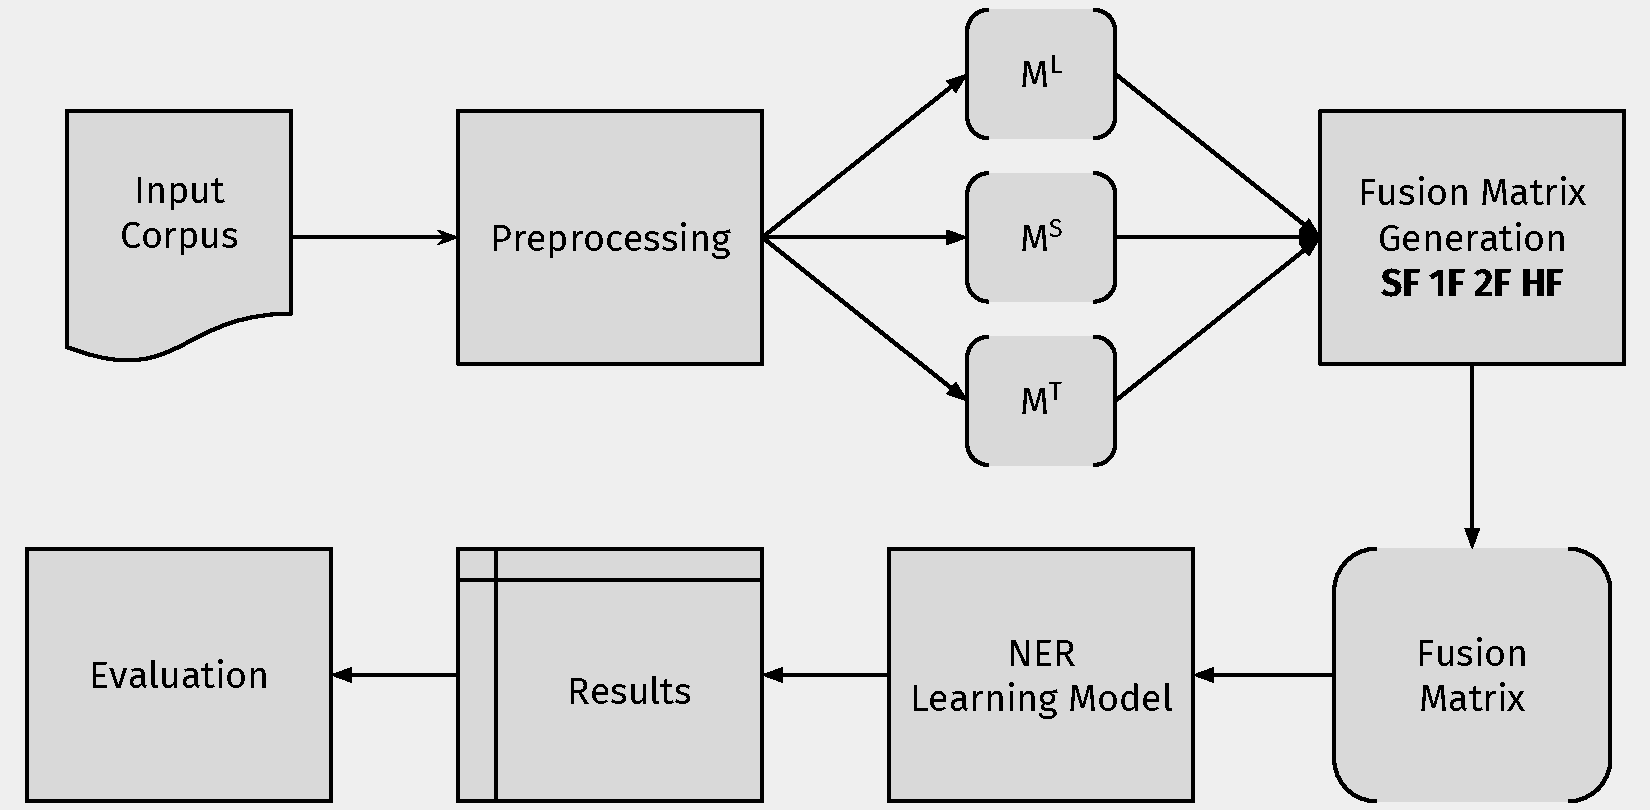
\includegraphics[width=0.85\linewidth]{image2/Chapitre4/diag_metodoNER.pdf}
%\end{frame}


\begin{frame}{Representation Spaces}
\hfill
\begin{itemize}
	\item[] \large \textbf{Example Phrase}
	\begin{itemize}
	\item[] \large \textit{Australian scientist discovers star with telescope}
	\end{itemize} 
\end{itemize}
\hfill
\begin{itemize}
\item[] \large \textbf{Three different types of features}
\end{itemize}

\small

\begin{tabular}{llr}

	\hline 
	 \textbf{Word} & \textbf{Features} & \textbf{Feature Type}\\ 
	\hline 
	Australian & word:Australian, word+1:scientist, ...& \textbf{Lexical (L)}\\ 
	scientist  &  Australian/JJ/amod, discovers/VBZ/nsubj\_inv & \textbf{Syntactic (S)}\\ 
	discover &discover, no-capital-letter, prf:dis, suf:ver, VBZ & \textbf{Standard (T)}\\ 
	\hline 
\end{tabular} 
\vspace{\textheight}
\end{frame}


%\begin{frame}{Representation Spaces}
%	\large \textbf{Syntactic Space (S)}
%	\vspace{1cm}
%	\small
%	
%	
%	\begin{tabular}{ll}
%	\hline 
%	 Word & Contexts \\ 
%	\hline 
%	Australian & scientist/NN/amod\_inv \\ 
%	scientist  &  Australian/JJ/amod, discovers/VBZ/nsubj\_inv\\ 
%	discovers & scientist/NN/nsubj, star/NN/dobj, telescope/NN/nmod:with \\ 
%	star & discovers/VBZ/dobj\_inv \\ 
%	telescope  &  discovers/VBZ/nmod:with\_inv \\ 
%	\hline \
%	\end{tabular} 
%	 
%	\vspace{\textheight}
%\end{frame}
%


%\begin{frame}{Representation Spaces}
%	\large \textbf{Standard Features Space (T)}
%	\vspace{1cm}
%	\begin{itemize}
%		\item Each word
%		\item Whether it is capitalized
%		\item Prefix and suffix (of each word their surroundings)
%		\item Part of Speech tag
%	\end{itemize}	 
%	\vspace{\textheight}
%\end{frame}



\begin{frame}{Experimental Protocol}
	\begin{itemize}
		\item<1-> \large \textbf{Preprocessing}
			\begin{itemize}
				\item<1-> Normalize numbers
			\end{itemize}
		\item<2-> \textbf{Test Corpora}
			\begin{itemize}
			\item<2-> CoNLL-2003 (CONLL): Train: 219,554 lines. Test: 50,350 lines
			\item<2-> Wikiner (WNER): 3.5 million words. 
			\item<2-> Wikigold (WGLD): 41,011 words. 
			\end{itemize}
		\item<3-> \textbf{Learning Algorithm}
			\begin{itemize}
				\item<3-> Structured Perceptron 
			\end{itemize}

		\item<4-> \textbf{Evaluation Metric}
			\begin{itemize}
				\item<4-> F-measure
				\item<4-> Evaluated with a 5-fold CV (WNER and WGLD)
			\end{itemize}
	\end{itemize}	 
	\vspace{\textheight}
\end{frame}


\begin{frame}[t]{Evaluation}
\begin{columns}
	\column{0.5\textwidth}
	\begin{minipage}[c][.8\textheight][c]{\linewidth}
	
	\onslide<1->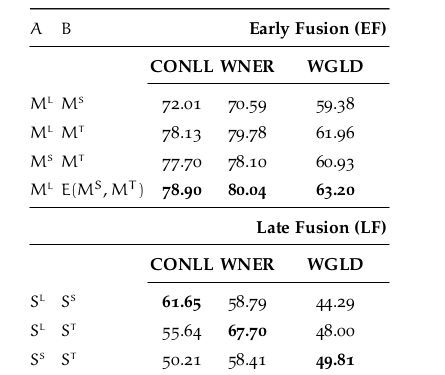
\includegraphics[width=1\linewidth]{image2/Chapitre4/1F_1.png}
	
	\end{minipage}
	\column{0.5\textwidth}
	\begin{minipage}[c][0.8\textheight][c]{\linewidth}
	\onslide<2->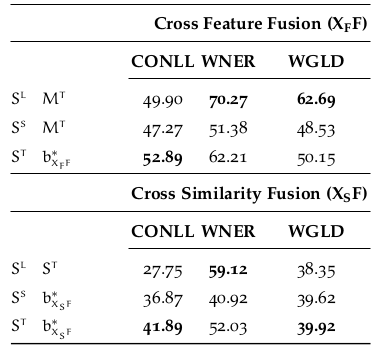
\includegraphics[width=1\linewidth]{image2/Chapitre4/1f_2.png}
	\\
	$b^*_{X_FF} \in \{\mlex, \mstd\}$
	\\
	$b^*_{X_SF} \in \{\slex, \ssyn\}$
	\end{minipage}
	\end{columns}
\end{frame}

\begin{frame}[t]{Evaluation}

%\begin{itemize}
%\item Best Fusion operators on the F-measure over the three datasets.  
%\item Achieved using a higher Degree fusion operator
%\item Notice the comparison with the Early Fusion baseline
%\item Visually show the best fusion operator, not with the formula.
%\end{itemize}



\begin{center}
\begin{itemize}
\onslide<1->\item[] \includegraphics[width=1\linewidth]{image2/Chapitre2/hybrid_fusiona_trim.pdf}%lexical
\onslide<2->\item[] \includegraphics[width=1\linewidth]{image2/Chapitre4/hf_trim.png}
\end{itemize}




\end{center}



\vspace{\textheight}
\end{frame}

\begin{frame}{Analyzing the Best Fusion Operator}
\begin{itemize}[<+- | alert@+>]
\item  \textbf{Understand how the evolution towards and enriched space helps the model take the correct decision}
\begin{itemize}
\item Decompose the large fusion operator into 4 separate representations
\item Train a model with each individual operator (4 models: $M_1$, $M_2$, $M_3$, $M_4$)
\item Investigate how the features added at each step help the model predict the correct class
\end{itemize}
\item[] \begin{equation*}
\overbrace{\underbrace{\overbrace{E_{\alpha=0.95}(\underbrace{\mlex}_{\circled{1}},\mstd}^{\circled{2}},L(\mstd, X_F(\ssyn, \mstd))}_{\circled{3}}, L(\mlex, X_F(\ssyn, \mlex))}^{\circled{4}})
\end{equation*}

\end{itemize}


%\begin{enumerate}
%\item[\circled{1}] $\mlex$ \label{eq:f1} used to train model $M_1$.
%\item[\circled{2}] $E(\alpha_1\mlex, \alpha_2\mstd)$ \label{eq:f2} used to train model $M_2$, with $\alpha_1=0.95,\alpha_2=0.05$
%\item[\circled{3}] $E_\alpha(\alpha_1\mlex, \alpha_2\mstd, \alpha_3L(\mstd, X_F(\ssyn, \mstd)))$ used to train model $M_3$, with $\alpha_1=0.95,\alpha_2=\alpha_3=0.05$
%\item[\circled{4}] $E_\alpha(\alpha_1\mlex, \alpha_2\mstd, \alpha_3L(\mstd, X_F(\ssyn, \mstd)), \alpha_4L(\mlex, X_F(\ssyn, \mlex)))$ used to train model $M_4$, with $\alpha_1=0.95,\alpha_2=\alpha_3=\alpha_4=0.05$
%\end{enumerate}
\end{frame}


\begin{frame}{Analyzing the Best Fusion Operator}
\large \textbf{We focus on the word \textit{Kory}, and its performance from model $M_1$ to $M_2$}
\begin{center}
\includegraphics[width=0.6\linewidth]{image2/Chapitre4/fanal1.png}
\end{center}
\end{frame}


\begin{frame}{Analyzing the Best Fusion Operator}
\large \textbf{We focus on the word \textit{Green}, and its performance from model $M_3$ to $M_4$}
\begin{center}
\includegraphics[width=0.6\linewidth]{image2/Chapitre4/fanalm3_m4.png}
\end{center}
\end{frame}

\section[Applications to NLP]{Solving Word Sense Induction and Disambiguation}

\begin{frame}{Introduction}
\begin{itemize}
\item<1-> \large \textbf{WSI/WSD Objective}
\begin{itemize}
\item<1->  The goal is to determine a set of possible senses to a given word according to its possible contexts (WSI). Then, assigning a correct sense to a particular instance of said word

\end{itemize}
\item<2-> \large \textbf{Our goals}
\begin{itemize}
\item<2-> Assess the effectiveness of the fusion enriched spaces
\item<2-> Evaluate the pertinence of our community discovering algorithm
\end{itemize}

\end{itemize}
\end{frame}


\begin{frame}{Experimental Protocol}
	\begin{itemize}
		\item<1-> \large \textbf{Preprocessing}
			\begin{itemize}
				\item<1-> Remove very frequent and very infrequent words
			\end{itemize}
		\item<2-> \textbf{Test Corpora}
			\begin{itemize}
			\item<2-> Semeval 2007 \cite{SangM03}: Train: 219,554 lines. Test: 50,350 
			\end{itemize}
		\item<3-> \textbf{Clustering Algorithm}
			\begin{itemize}
				\item<3-> Spectral Clustering \cite{Shi2000}
				\item<3-> Proposed Community Algorithm
			\end{itemize}

		\item<4-> \textbf{Evaluation Metrics}
			\begin{itemize}
				\item<4-> Supervised Recall
				\item<4-> Unsupervised  F-measure
				\item<5-> Proposed: H-measure
				\begin{itemize}
				\item<5->[] \includegraphics[width=0.6\linewidth]{image2/Chapitre4/h-measure}
				\item<5->[] \small $\delta$ is the average true number of senses of the words in a test corpus

				\end{itemize}
			\end{itemize}
	\end{itemize}	 
	\vspace{\textheight}
\end{frame}

\begin{frame}{Spectral Clustering Evaluation}
\begin{columns}
	\column{0.5\textwidth}
	\begin{minipage}[c][0.5\textheight][c]{\linewidth}
	\onslide<1->
	\begin{figure}
		\centering
		\includegraphics[width=1\linewidth]{image2/Chapitre4/wsd_SC_SR}
		\caption{Supervised Recall}
	\end{figure}

	\end{minipage}
	\column{0.5\textwidth}
	\begin{minipage}[c][0.5\textheight][c]{\linewidth}
	\onslide<2->
	\begin{figure}
		\centering
		\includegraphics[width=1\linewidth]{image2/Chapitre4/wsd_SC_UF.png}
		\caption{Unsupervised F-measure}
	\end{figure}
	\end{minipage}
	\end{columns}
\end{frame}



\begin{frame}{Spectral Clustering Evaluation}
\begin{figure}
	\centering
	\includegraphics[width=.6\linewidth]{image2/Chapitre4/wsd_SC_Hm.png}
	\caption{Proposed H-measure}
\end{figure}
\end{frame}


\begin{frame}{Proposed Algorithm Evaluation}
\begin{columns}
	\column{0.5\textwidth}
	\begin{minipage}[c][0.5\textheight][c]{\linewidth}
	\onslide<1->
	\begin{figure}
		\centering
		\includegraphics[width=1\linewidth]{image2/Chapitre4/wsd_PA_SR}
		\caption{Supervised Recall}
	\end{figure}

	\end{minipage}
	\column{0.5\textwidth}
	\begin{minipage}[c][0.5\textheight][c]{\linewidth}
	\onslide<2->
	\begin{figure}
		\centering
		\includegraphics[width=1\linewidth]{image2/Chapitre4/wsd_PA_UF.png}
		\caption{Unsupervised F-measure}
	\end{figure}
	\end{minipage}
	\end{columns}
\end{frame}


\begin{frame}{Proposed Algorithm Evaluation}
\begin{figure}
	\centering
	\includegraphics[width=.5\linewidth]{image2/Chapitre4/wsd_PA_Hm.png}
	\caption{Proposed H-measure}
\end{figure}
\end{frame}





%
%
%\item\textbf{ How can we improve the model?}
%\begin{itemize}
%\item Leverage large sources of text data to enrich current approach
%\item Combine the information stored in the HLM
%\item Improve the WSD stage
%\item Select other more pertinent similarity measures
%
%\end{itemize}
%





%
%


%\section{Ongoing Work}
%
%
%
%\begin{frame}{Combining linguistic features: Information Fusion}
%%			\item By projecting robust information from the syntactic dependencies hypergraph incidence matrix towards the lexical co-occurrence incidence matrix, via the dot product, we can propagate the information contained in the first matrix into the second and thus find more relevant semantic relations between words.
%%			
%%			\begin{figure}
%%			\centering
%%			\includegraphics[width=0.4\linewidth]{img/cross}
%%			\end{figure}
%
%
%	\begin{columns}
%	\column{.5\textwidth}
%	\begin{minipage}[c][0.4\textheight][c]{\linewidth}
%	  \centering
%	  \begin{itemize}
%		  \item \textbf{Inspired on the image/text fusion literature \cite{Snoek2005,ah2015unsupervised}:}
%		  \begin{itemize}
%			  \item Early fusion
%			  \item Late fusion
%			  \item \textbf{Cross fusion}
%		  
%		  \end{itemize}
%	  
%	  \end{itemize}
%	\end{minipage}
%	\column{.5\textwidth}
%	\begin{minipage}[c][0.4\textheight][c]{\linewidth}
%		\centering
%		\includegraphics[width=1\linewidth]{img/cross}
%	\end{minipage}
%	\end{columns}
%
%			
%\end{frame}
%


\metroset{sectionpage=none}
\metroset{sectionpage=progressbar}
\section{Conclusions}

\begin{frame}{Insights From our Contributions}
\begin{itemize}
\item<1-> \textbf{Hypergraph linguistic model to hold heterogeneous information}
	\begin{itemize}
		\item<1-> Hypergraphs allow a  multi-layered representation of text within a single resource. 
		\item<1-> The Wikipedia-based instantiation serves as a NLP system starting point
		
	\end{itemize}
\item<2-> \textbf{Multimedia fusion techniques to combine and densify representations}
	\begin{itemize}
	\item<2-> High-degree combinations of linguistic representations reduce sparsity 
	\item<2-> These fusion spaces achieve improvements on NER and WSI/WSD compared to single features and trivial fusion

	\end{itemize}
\item<3-> \textbf{Finding semantically-related communities on linguistic networks}
		\begin{itemize}	
		\item<3-> The proposed community finding method improves over similar algorithms while being simpler and allowing for heterogeneous features
		\end{itemize}
\end{itemize}


\end{frame}

\begin{frame}{Future Work}
\begin{itemize}
\item<1-> \textbf{Hypergraph Linguistic Model}
	\begin{itemize}
	\item<1-> A  dataframe-like structure specialized on linguistic information based on the proposed model
	\item<1-> Defining inter-features similarities measures within the network
	\end{itemize}
\item<2-> \textbf{Combining Features and Dealing with Sparsity}
	\begin{itemize}
	\item<2-> Finding a more principled way to determine what type of
		context with what type of fusion operation according to the task at hand
	\item<2-> Exploring fusion with other types of features (other modalities)  
	\end{itemize}
\item<3-> \textbf{Applications to NLP}
	\begin{itemize}
	\item<3-> Comparison with other distributional representations (word embeddings)
	\item<3-> Using the large Wikipedia-based network as a background corpus to further enrich domain-specific corpora
	\item<3-> Test more feature weighting schemes, validate findings on more datasets
	\end{itemize}
\end{itemize}


\end{frame}




\begin{frame}{Publications Produced by our Research}
\begin{itemize}
	\item \footnotesize Edmundo-Pavel Soriano-Morales, Julien Ah-Pine, Sabine Loudcher: \textbf{Fusion Techniques for Named Entity Recognition and Word Sense Induction and Disambiguation}. DS 2017
	\item \footnotesize Edmundo-Pavel Soriano-Morales, Julien Ah-Pine, Sabine Loudcher:
	\textbf{Using a Heterogeneous Linguistic Network for Word Sense Induction and Disambiguation.} CICLING 2016
	\item \footnotesize Edmundo-Pavel Soriano-Morales, Julien Ah-Pine, Sabine Loudcher:
		\textbf{Hypergraph Modelization of a Syntactically Annotated English Wikipedia Dump}. LREC 2016
	\item \footnotesize Adrien Guille, Edmundo-Pavel Soriano-Morales, Ciprian-Octavian Truica:
\textbf{Topic modeling and hypergraph mining to analyze the EGC conference history}. EGC 2016
\item \footnotesize Adrien Guille, Edmundo-Pavel Soriano-Morales:
\textbf{TOM: A library for topic modeling and browsing.} EGC 2016
\item \footnotesize Julien Ah-Pine, Edmundo-Pavel Soriano-Morales: \textbf{A Study of Synthetic Oversampling for Twitter Imbalanced Sentiment Analysis}. DMNLP@PKDD/ECML 2016

\item \footnotesize Sabine Loudcher, Wararat Jakawat, Edmundo-Pavel Soriano-Morales, C\'{e}cile Favre:	\textbf{Combining OLAP and information networks for bibliographic data analysis: a survey}. Scientometrics 103(2) 2015
\end{itemize}
\end{frame}

\setbeamertemplate{frametitle}
{
    \nointerlineskip
    \begin{beamercolorbox}[sep=0.3cm,ht=2.5em,wd=\paperwidth]{frametitle}
        \vbox{}\vskip-2ex%
        \strut\hfill\insertframetitle\hfill\strut
        \vskip-0.8ex%
    \end{beamercolorbox}
}

\begin{frame}{\textcolor{greenEric}{Thank you for your attention}}
\begin{itemize}
	\item \footnotesize Edmundo-Pavel Soriano-Morales, Julien Ah-Pine, Sabine Loudcher: \textbf{Fusion Techniques for Named Entity Recognition and Word Sense Induction and Disambiguation}. DS 2017
	\item \footnotesize Edmundo-Pavel Soriano-Morales, Julien Ah-Pine, Sabine Loudcher:
	\textbf{Using a Heterogeneous Linguistic Network for Word Sense Induction and Disambiguation.} CICLING 2016
	\item \footnotesize Edmundo-Pavel Soriano-Morales, Julien Ah-Pine, Sabine Loudcher:
		\textbf{Hypergraph Modelization of a Syntactically Annotated English Wikipedia Dump}. LREC 2016
	\item \footnotesize Adrien Guille, Edmundo-Pavel Soriano-Morales, Ciprian-Octavian Truica:
\textbf{Topic modeling and hypergraph mining to analyze the EGC conference history}. EGC 2016
\item \footnotesize Adrien Guille, Edmundo-Pavel Soriano-Morales:
\textbf{TOM: A library for topic modeling and browsing.} EGC 2016
\item \footnotesize Julien Ah-Pine, Edmundo-Pavel Soriano-Morales: \textbf{A Study of Synthetic Oversampling for Twitter Imbalanced Sentiment Analysis}. DMNLP@PKDD/ECML 2016

\item \footnotesize Sabine Loudcher, Wararat Jakawat, Edmundo-Pavel Soriano-Morales, C\'{e}cile Favre:	\textbf{Combining OLAP and information networks for bibliographic data analysis: a survey}. Scientometrics 103(2) 2015
\end{itemize}
\end{frame}

%

%\begin{frame}[allowframebreaks]{References}

%\printbibliography
%\bibliographystyle{alpha}

%\end{frame}	
	
\end{document}
